\documentclass[a4paper,twoside,12pt]{book}
\usepackage[utf8]{inputenc}
\usepackage[T1]{fontenc}
\usepackage{wrapfig}
\usepackage{graphicx}
\usepackage{lscape}
\usepackage{amsmath}
\usepackage{amssymb}
\usepackage{lmodern}
\usepackage{fancyhdr}
\usepackage{titlesec}
\usepackage{tocbibind}
\usepackage[round,colon,authoryear]{natbib}
\def\bibfont{\small}
\bibpunct{(}{)}{,}{a}{}{}
\usepackage{url}
\usepackage[font=footnotesize,format=plain,labelfont=bf,up,textfont=up]{caption}
\usepackage[top=3.5cm,bottom=3cm,left=3.2cm,right=3.2cm,headsep=1.2cm,footnotesep=1.2cm]{geometry}
\usepackage[plainpages=false,backref,bookmarks=true,hypertexnames=false,colorlinks=true,linkcolor=blue,urlcolor=blue,citecolor=blue]{hyperref}
\usepackage{bookmark}
\bookmarksetup{startatroot}
\usepackage{minitoc}
\usepackage[french]{babel}
\usepackage{tcolorbox}
\usepackage{subfig}
\usepackage{pifont}
\usepackage{hyperref}
\usepackage{multirow}
\usepackage{gensymb}
\usepackage{pdflscape}
\usepackage[final]{pdfpages}
\usepackage{xcolor}
\usepackage{threeparttable}
\usepackage{arabtex}

%%%%%%%%%%%%%%%%%%%%



%%%%%%%%%%%%%%%%%%%%%%%%%%%%%
\renewcommand{\headrulewidth}{0.5pt}
\renewcommand{\footrulewidth}{0pt}

% rules, no headings
\fancypagestyle{fancyempty}{
    \fancyhf{}
    \fancyhead[LE,RO]{\bfseries\thepage}
    \fancyhead[LO]{}
    \fancyhead[RE]{}
    \addtolength{\headheight}{0.5pt}}
% empty
\fancypagestyle{empty}{
    \fancyhead{}\renewcommand{\headrulewidth}{0pt}}
% full headings
\pagestyle{fancy}
\renewcommand{\chaptermark}[1]{\markboth{\ #1}}
%\renewcommand{\sectionmark}[1]{\markright{\ #1}}
\renewcommand{\chaptermark}[1]{\markright{\ #1}}
\fancypagestyle{plain}{
    \fancyhf{}
    \fancyhead[LE,RO]{\bfseries\thepage}
    \fancyhead[LO]{\nouppercase\rightmark}
    \fancyhead[RE]{\nouppercase\rightmark}
    %\fancyhead[RE]{\nouppercase\leftmark}
    \addtolength{\headheight}{0.5pt}}

% MARGINS
\titlespacing*{\chapter}{0pt}{-40pt}{20pt}
\titleformat{\chapter}[display]{\normalfont\huge\bfseries}{\chaptertitlename\ \thechapter}{30pt}{\Huge}
\titleformat{\paragraph}[display]{\normalfont\itshape}{\paragraphtitlename\ \theparagraph}{}{}

% CHAPTER HEADINGS
\makeatletter
\def\thickhrulefill{\leavevmode \leaders \hrule height 1ex \hfill \kern \z@}
\def\@makechapterhead#1{%
  \reset@font
  \parindent \z@
  \vspace*{5\p@}%
  \hbox{%
    % BOX
    \vbox{\hsize=2.5cm
      \begin{tabular}{c}
        \scshape \strut \@chapapp{} \\
        \fbox{%
          \vrule depth 3em height 4em width 0pt%
          \vrule height 0pt depth 0pt width 2ex%
          {\fontsize{48}{0}\selectfont \bfseries \strut \thechapter}%
          \vrule height 0pt depth 0pt width 1ex%
          }
      \end{tabular}%
      }%
    % CHAPTER TITLE
    \vbox{%
      \advance\hsize by -2.5cm
      \hrule\par
      \vskip 5pt%
      \flushright
      \huge \bfseries #1
      \vskip 5pt%
      \hrule\par
      }%
    }%
  \vskip 10\p@
  \setlength{\parindent}{18pt}
}
% CHAPTER*
\def\@makeschapterhead#1{%
  \reset@font
  \parindent \z@
  \vspace*{10\p@}%
  \hbox{%
    \vbox{%
      \hrule\par
      \vskip 10pt%
      \flushright
      \huge \bfseries #1
      \vskip 10pt%
      \hrule\par
      }%
    }%
  \vskip 50\p@
  \setlength{\parindent}{18pt}
}
% PART
\newcommand\newpart[1]{
% ============
\part*{#1}
}
\def\@spart#1{%
% ============
\thispagestyle{fancyempty}
\vspace*{100\p@}
\hbox{
\vbox{
  % \hrule\par
  \vskip 10pt
  \flushright
  \fontsize{36}{0} \bfseries {#1}
  \vskip 8pt
  \hrule\par }
}
\vskip 50\p@
\adjustmtc
\mtcaddpart[#1]
}

% CHAPTER ABSTRACT
\def\chapterabstract#1{
    % ABSTRACT
    {\noindent\large \bfseries Inroduction}
    \vspace{0.2cm}
    \hrule
    \vspace{0.3cm}
    \noindent\textit{#1}
    \vspace{0.3cm}
    \hrule
    \vspace{0.5cm}
    \minitoc
    \newpage
}
\makeatother

% Problème de césure des mots
\tolerance=1
\emergencystretch=\maxdimen
\hyphenpenalty=10000
\hbadness=10000


% BEGIN DOCUMENT
\begin{document}
\frontmatter
\pagestyle{fancyempty}

 \title{The Title}
 \author{Mohammed AMEKSA}



\begin{titlepage}

\includepdf[pages=-]{pageDeGard/pageDeGardRec.pdf}
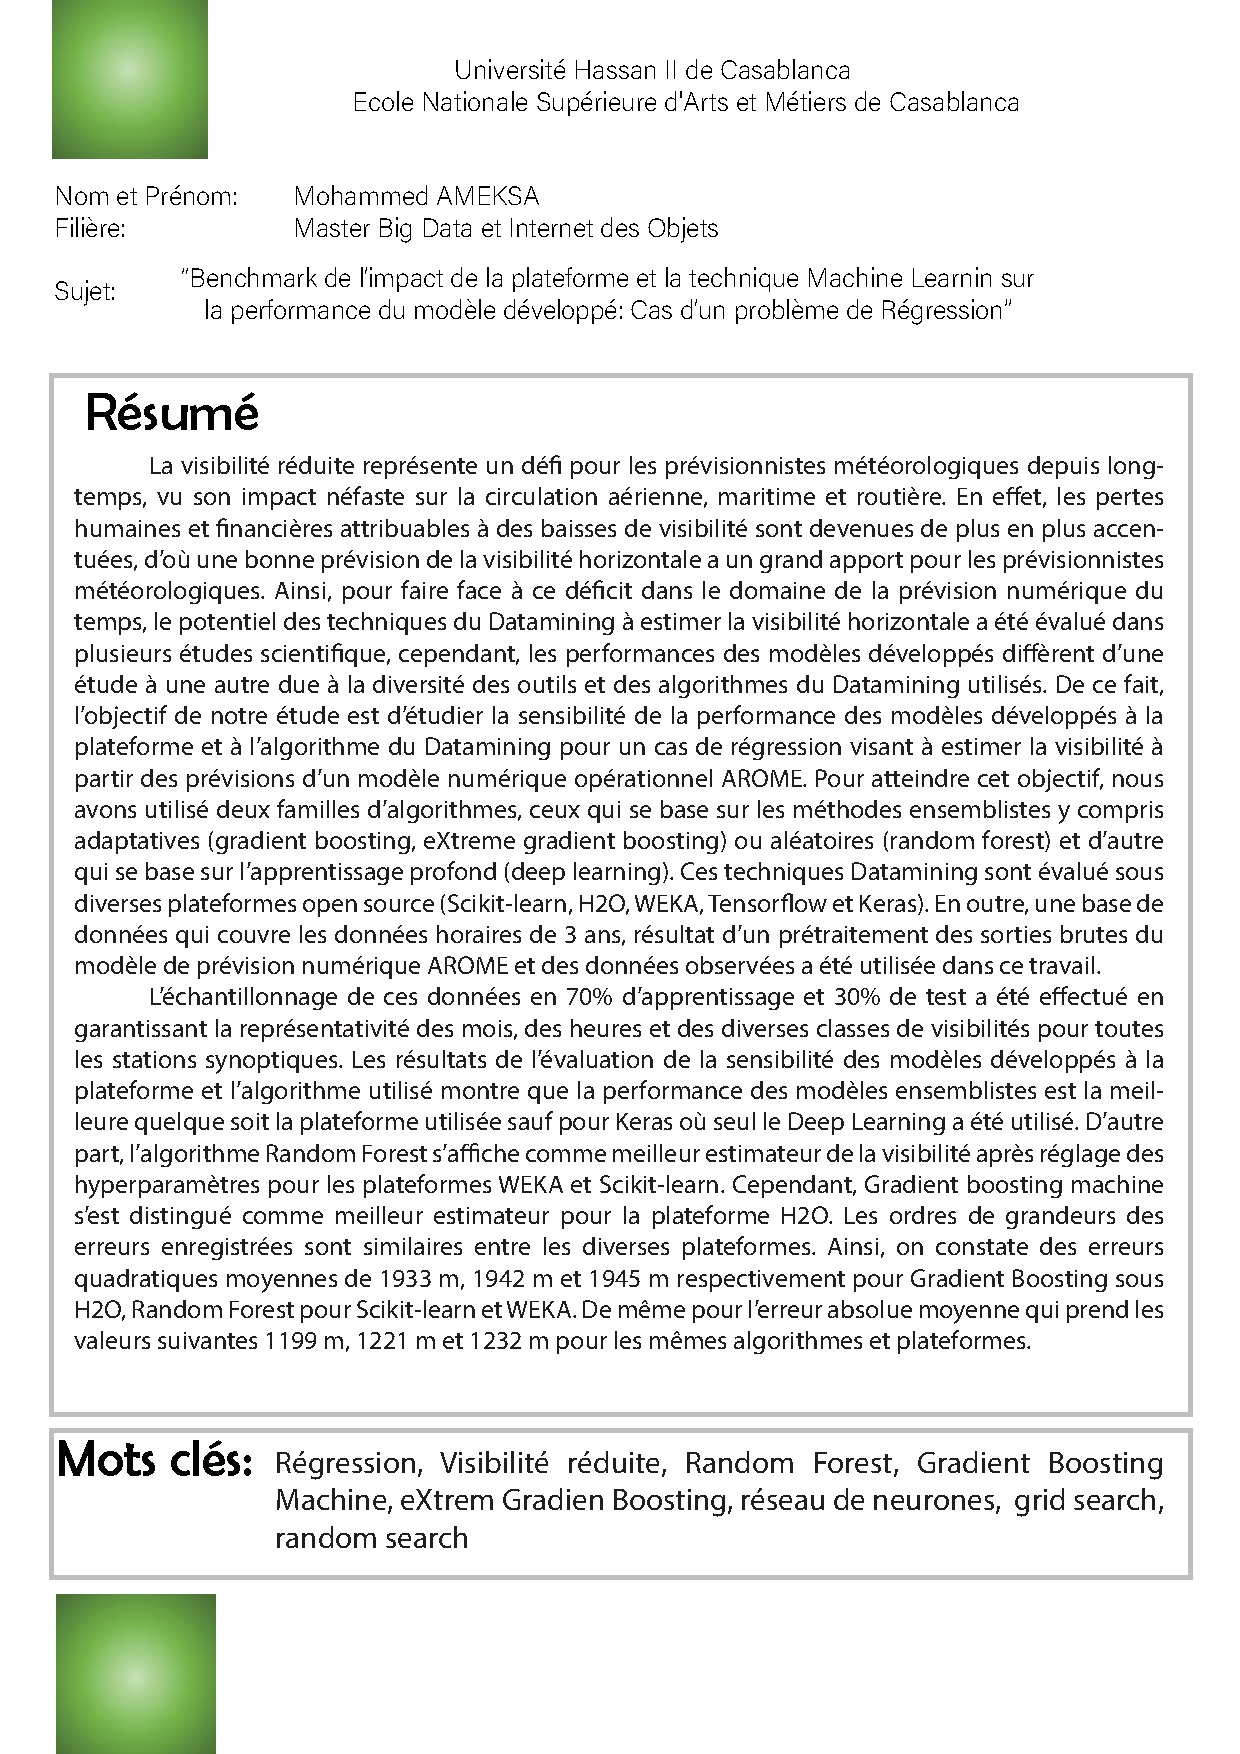
\includepdf[pages=-]{pageDeGard/pageDeGardVers.pdf}
\end{titlepage}

\thispagestyle{empty}

\newpage

% PREAMBULE
\dominitoc



\setcounter{page}{1}
\chapter*{Dédicaces}
\mtcaddchapter[Dédicaces]
\label{chap:didicace}
\textit{À celle qui a attendu avec impatience les fruits de sa bonne éducation, à ma mère.\\
À celui qui m'a indiqué la bonne voie en me rappelant que la volonté fait toujours les grands hommes, à mon père.\\
En témoignage de ma profonde gratitude et de mon incontestable reconnaissance envers vous.\\
À mes sœurs auprès desquelles j'ai trouvé un soutien sans complaisance et des encouragements sincères.\\
À ceux qui m'ont donné un coup de main et m'ont accueilli parmi leurs enfants au cours de mes études.\\
À toute ma famille et mes amis qui ont fait preuve de soutien et qui m’ont donné une motivation sans prix.\\
À ceux et celles qui ont quitté l'école à cause de la difficulté des circonstances et des conditions.\\
À chaque enseignant et professeur qui a fait de son mieux pour des fins éducatives.\\
À toutes les personnes qui ont cru en mes succès.}

\let\cleardoublepage\clearpage
\chapter*{Remerciements}
\mtcaddchapter[Remerciements]
\label{chap:Remerciements}
Je remercie d’abord Dieu pour ses bienfaits trop souvent négligés. Ensuite,  m’est agréable de s'acquitter d'une dette de reconnaissance auprès de toutes les personnes, dont l'intervention au cours de ce projet a favorisé son aboutissement.\\


Mes très chers remerciements vont à M. Driss BARI, mon encadrant au sein de la Direction de la Météorologie Nationale (DMN) Casablanca, qui n’a pas manqué de me préparer les conditions favorables au bon déroulement du projet. Toute ma gratitude envers lui pour son  accueil chaleureux au sein de la DMN, pour le fait de me proposer un tel sujet captivant et intéressant qui m'a permis de vivre une expérience professionnelle avantageuse et enrichissante. Ainsi, pour ses explications et pour ses conseils qu’il m'a prodigués et son judicieux encadrement. Aussi bien son aide dans la rédaction de ce rapport.\\


Mes remerciements les plus sincères vont aussi à M. Youssef TAHIR d'avoir encadré mon Projet de Fin d'études (PFE), je le remercie vivement pour sa disponibilité et tous ses conseils, durant les différentes phases du projet ainsi que son aide dans la rédaction de ce rapport.\\


Mes plus vifs remerciements sont aussi adressés au personnel de la DMN, pour l'intérêt qu'ils m'ont apporté durant ces quatre mois de stage.\\


Je tiens à exprimer mes gratitudes à toute l’équipe pédagogique et tout le corps professoral de l'École Nationale Supérieure d'Arts et Métiers (ENSAM) de Casablanca d'avoir porté un vif intérêt à ma formation, et pour avoir accordé le plus clair de leur temps, leur attention et leur énergie et ce dans un cadre agréable de complicité et de respect.\\


Enfin, que tous ceux et celles qui ont contribué de près ou de loin à l'accomplissement de ce travail trouvent l'expression de mes remerciements les plus chaleureux.
\let\cleardoublepage\clearpage
\chapter*{Résumé}
\mtcaddchapter[Résumé]
\label{chap:abstract_fr}
La visibilité réduite représente un défi pour les prévisionnistes météorologiques depuis longtemps, vu son impact néfaste sur la circulation aérienne, maritime et routière. En effet, les pertes humaines et financières attribuables à des baisses de visibilité sont devenues de plus en plus accentuées, d'où une bonne prévision de la visibilité horizontale a un grand apport pour les prévisionnistes météorologiques. Ainsi, pour faire face à ce déficit dans le domaine de la prévision numérique du temps, le potentiel des techniques du Datamining à estimer la visibilité horizontale a été évalué dans plusieurs études scientifique, cependant, les performances des modèles développés diffèrent d'une étude à une autre due à la diversité des outils et des algorithmes du Datamining utilisés. De ce fait, l'objectif de notre étude est d'étudier la sensibilité de la performance des modèles développés à la plateforme et à l'algorithme du Datamining pour un cas de régression visant à estimer la visibilité à partir des prévisions d'un modèle numérique opérationnel AROME.
Pour atteindre cet objectif, nous avons utilisé deux familles d'algorithmes, ceux qui se base sur les méthodes ensemblistes y compris adaptatives (\textit{gradient boosting}, \textit{eXtreme gradient boosting}) ou aléatoires (\textit{random forest}) et d'autre qui se base sur l'apprentissage profond (\textit{deep learning}). Ces techniques Datamining sont évalué sous diverses plateformes open source (\textit{Scikit-learn}, \textit{H2O}, \textit{WEKA}, \textit{Tensorflow} et \textit{Keras}). En outre, une base de données qui couvre les données horaires de 3 ans, résultat d’un prétraitement des sorties brutes du modèle de prévision numérique AROME et des données observées a été utilisée dans ce travail. L’échantillonnage  de  ces  données  en  70\% d'apprentissage et 30\% de test  a été effectué en garantissant la représentativité des mois, des heures et des diverses classes de visibilités pour toutes les stations synoptiques. Les résultats de l'évaluation de la sensibilité des modèles développés à la plateforme et l'algorithme utilisé montre que la performance des modèles ensemblistes est la meilleure quelque soit la plateforme utilisée sauf pour \textit{Keras} où seul le \textit{Deep Learning} a été utilisé. D'autre part, l’algorithme \textit{Random Forest} s’affiche comme meilleur estimateur de la visibilité après réglage des hyperparamètres pour les plateformes \textit{WEKA} et \textit{Scikit-learn}. Cependant, \textit{Gradient boosting machine} s’est distingué comme meilleur estimateur pour la plateforme \textit{H2O}. Les ordres de grandeurs des erreurs enregistrées sont similaires entre les diverses plateformes. Ainsi, on constate des erreurs quadratiques moyennes de 1933 m, 1942 m et 1945 m respectivement pour \textit{Gradient Boosting} sous \textit{H2O}, \textit{Random Forest} pour \textit{Scikit-learn} et \textit{WEKA}. De même pour l’erreur absolue moyenne qui prend les valeurs suivantes 1199 m, 1221 m et 1232 m pour les mêmes algorithmes et plateformes.

\let\cleardoublepage\clearpage
\chapter*{Abstract}
\mtcaddchapter[Abstract]
\label{chap:Abstract}
Low visibility has been a challenge for weather forecasters for a long time, due to its negative impact on air, sea and road traffic. Indeed, the human and financial losses attributable to reduced visibility become increasingly important, hence a good forecast of horizontal visibility is of great benefit to meteorological forecasters. So, to cope with this challenge in the area of numerical weather prediction, the potential of Datamining techniques to estimate horizontal visibility has been evaluated in several scientific studies. However, the performance of developed models differs from one study to another due to the variety of Datamining tools and algorithms used. Therefore, the objective of our study is to evaluate the sensitivity of the performance of the developed models to the Datamining platform and algorithm for a regression case which aims to estimate the visibility from the predictions of the operational numerical weather prediction AROME model. To achieve this goal, we used two types of algorithms : those based on the ensemble methods including \textit{gradient boosting}, \textit{eXtreme gradient boosting} and \textit{random forest}, and those based on \textit{deep learning}. The algorithms are evaluated under various open source platforms (\textit{Scikit-learn}, \textit{H2O}, \textit{WEKA}, \textit{Tensorflow} and \textit{Keras}). In addition, a database covering 3-year of hourly data, and resulting from preprocessing of the raw outputs of AROME and the observed data, was used in this work. The sampling of these data in 70\% for learning and 30\% for testing was carried out by guaranteeing the representativity of the months, the hours and the various classes of visibilities for all the synoptic stations. The results show that the performance of the models based on the ensemble methods is the best whatever the used platform except for \textit{Keras} where only the \textit{Deep Learning} was used. On the other hand, the \textit{Random Forest} algorithm is found as the best estimator of visibility after tuning of hyperparameters for the \textit{WEKA} and \textit{Scikit-learn} platforms. However, \textit{Gradient boosting machine} outperforms the other algorithms for the \textit{H2O} platform. Besides, the mean squared errors are 1933 m, 1942 m and 1945 m respectively for \textit{Gradient Boosting} under \textit{H2O}, \textit{Random Forest} for \textit{Scikit-learn} and \textit{WEKA}. Similarly for the mean absolute error took the following values 1199 m, 1221 m and 1232 m for the same algorithms and platforms.
\let\cleardoublepage\clearpage
\newpage
\mtcaddchapter[Résumé en arabe]
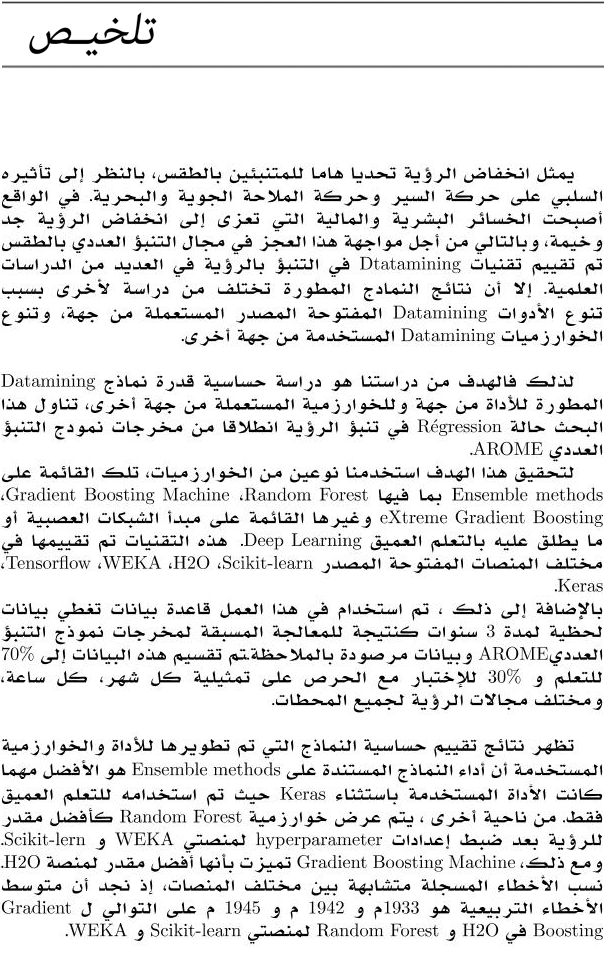
\includegraphics[width=14cm]{img/abstract_ar.png}
\let\cleardoublepage\clearpage
\chapter*{Table des Abréviations}
\mtcaddchapter[Table des Abréviations]
\label{chap:abreviations}
\begin{table}[h!]
        \centering
        \begin{tabular}{|p{2cm}p{8cm}|}
        \hline
        \multicolumn{2}{|c|}{Les abréviations}  \\ \hline
         DMN & Direction de la Météorologie Nationale  \\
         CPM & Centres Provinciaux Météorologiques \\
         CNRMSI & Centre Nationale de Recherche Météorologique et Systèmes d'Information\\
         WMO & Organisation Météorologique Mondiale\\
         PNT & Prévision Numérique du Temps\\
         CRQ & Comptes Rendus Quotidiens\\
         KDD & Knowledge Discovery from Databases\\
         RF & Random Forest  \\ 
         GBM & Gradient Boosting Machine \\
         XGB & eXtreme Gradient Boosting \\
         DL & Deep Learning \\
         MLP & MultiLayer Perceptron \\
         ACP & Analyse en Composantes Principales \\
         MAE & Mean Absolute Error \\
         RMSE & Root Mean Square Error \\
         CC & Correlation Coefficient\\
         
         \hline
        \end{tabular}
        \end{table}

\let\cleardoublepage\clearpage
\setcounter{secnumdepth}{3}
\setcounter{tocdepth}{2}
\markboth{}{}
\tableofcontents
\markboth{}{}

\listoffigures
\let\cleardoublepage\clearpage
\listoftables
\let\cleardoublepage\clearpage


% INTRODUCTION
\mainmatter

\markboth{}{}
\setcounter{mtc}{9}
\chapter[Introduction Générale]{Introduction Générale}
\label{Introduction}

\chapterabstract
{
Dans ce chapitre introductif, nous allons présenter d'une part l'organisme d'accueil « Direction de la Météorologie 
Nationale » où le stage a été effectué, ses stratégies, ses missions et ses domaines d'activité. D'autre part, 
nous présenterons aussi les enjeux liés à la prévision de la visibilité, ainsi que l’état des lieux en ce qui concerne 
l'estimation de la visibilité grâce au Datamining à partir de diverses sources de données en utilisant divers algorithmes dans différentes plateformes.
Les objectifs du stage et la stratégie suivie pour les atteindre seront explicités en fin de ce chapitre.
}
\pagestyle{plain}

%%%%%%%%%%%%%%%%%%%%%%%%%%%%%%%%%%%%%%%%%%%%%%%%%%%%%%%%%%%%%%%%%%%%%%%
\section{Organisme d’accueil: Direction de la Météorologie Marocaine}
%%%%%%%%%%%%%%%%%%%%%%%%%%%%%%%%%%%%%%%%%%%%%%%%%%%%%%%%%%%%%%%%%%%%%%%
\begin{wrapfigure}{l}{0.2\textwidth}
    \vspace{-0.5 cm}    
    
\includegraphics[width=0.2\textwidth]{img/logo_dmn.png}
    \vspace{-1 cm}
\end{wrapfigure}
A travers la Direction de la Météorologie Nationale (DMN, souvent appelé Maroc Météo par les usagers), le Maroc dispose d’un outil à même d'assurer et de coordonner l'ensemble des activités météorologiques et climatiques. La DMN, en tant que service public, a pour objectif central de promouvoir une assistance technique et scientifique dans les sciences de l'atmosphère. Sa mission est de servir les intérêts socio-économiques de la nation et de contribuer à la
sauvegarde des vies et des biens de la population, à travers son métier qui consiste en (Cf. Fig. \ref{fig:MissionDMN}) :
\begin{itemize}
\item[\ding{224}] l'observation et la mesure météorologiques,
\item[\ding{224}] la prévision,
\item[\ding{224}] la veille et le suivi du climat,
\item[\ding{224}] l'assistance météorologique aux secteurs économiques : la navigation aérienne, les activités marines, l'agro-météorologie, l'hydro-météorologie et l'environnement, etc.\\
\end{itemize}

\begin{figure}[!h]
\centering
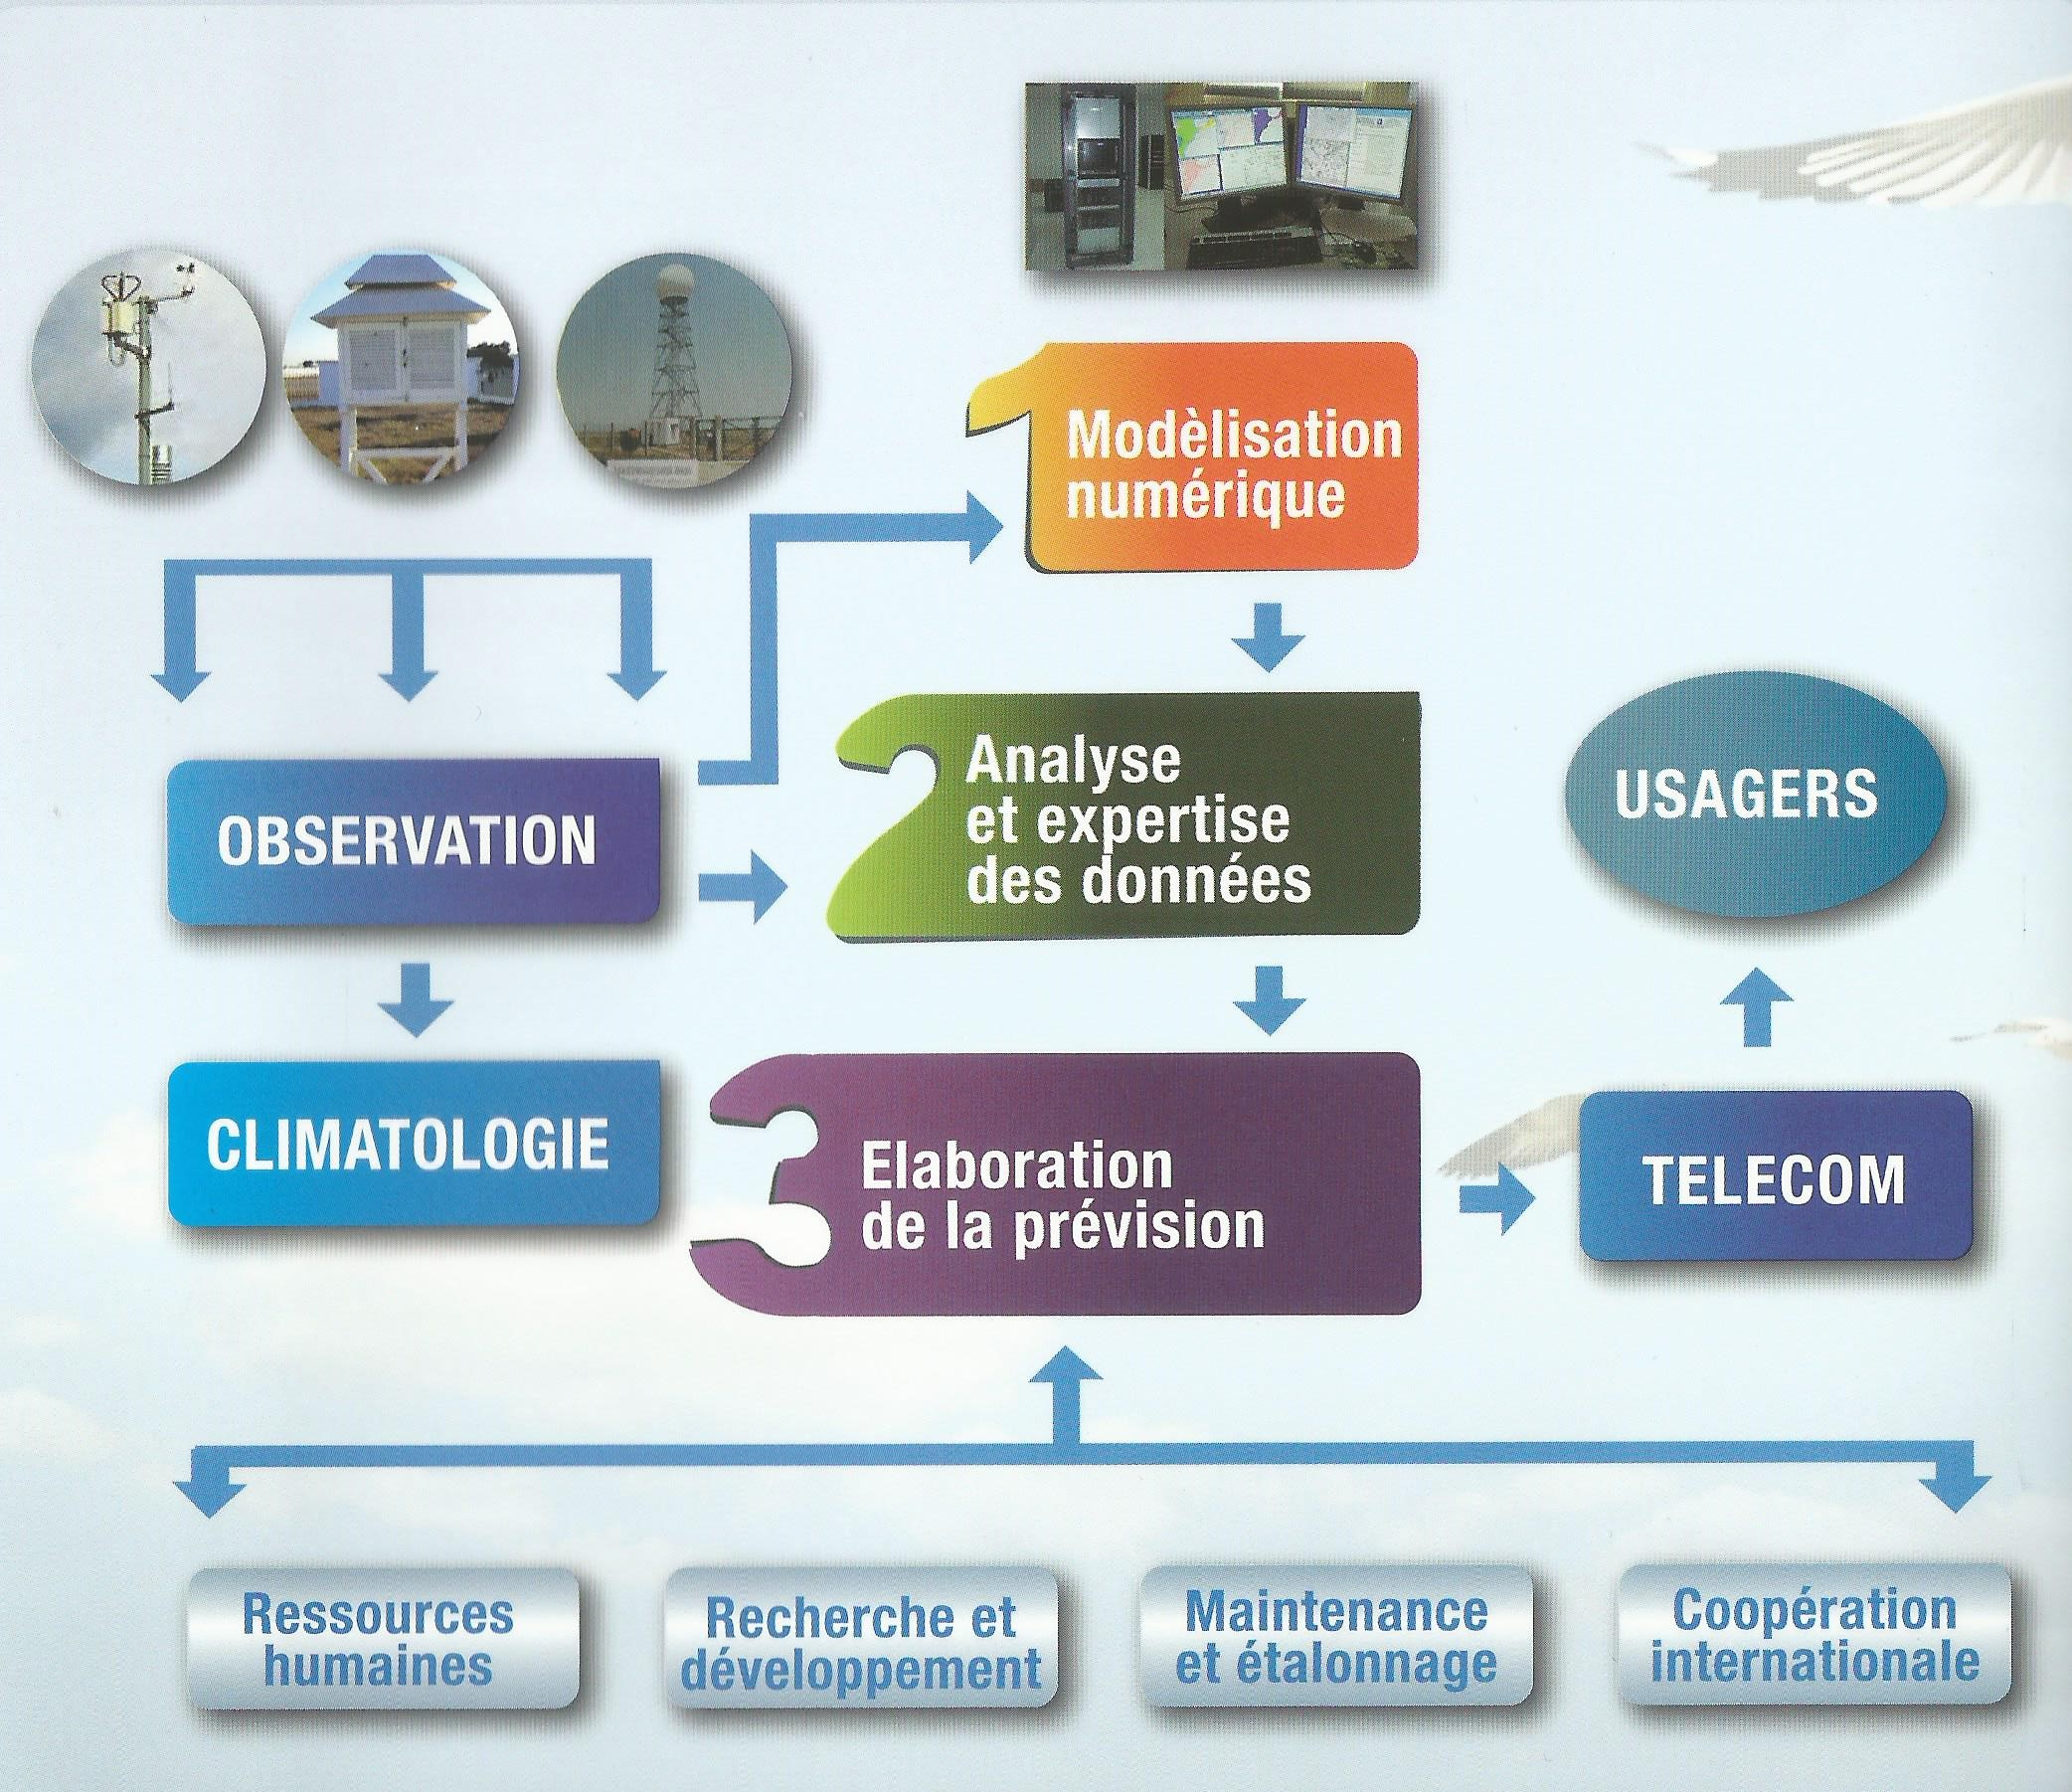
\includegraphics[width=10 cm, height= 7 cm]{img/DMN.jpeg}
\caption{Représentation schématique des principales activités de Maroc Météo}
\label{fig:MissionDMN}
\end{figure}

Les missions de la DMN décrites dans le décret No. 2-94-724 du 21 Novembre 1994 sont :
\begin{itemize}
\item[\ding{224}] Assurer les activités relatives aux
informations météorologiques et
climatologiques nécessaires pour satisfaire tous les besoins des usagers au plan national et assurer les échanges internationaux de données en application des
accords ratifiés par le Royaume du Maroc.
\item[\ding{224}] Effectuer des études et recherches atmosphériques, de météorologie et de
climatologie théoriques, expérimentales et appliquées ainsi que les études et les recherches connexes en rapport avec sa mission.
\item[\ding{224}] Participer à la préparation des accords internationaux en liaison avec les administrations intéressées concernant les domaines de sa compétence et
d’établir les textes réglementaires relatifs à la météorologie et en assurer l’exécution.\\
\end{itemize}
 
 Pour répondre à sa mission, Maroc Météo dispose de ressources humaines hautement qualifiées dans les domaines de la météorologie, de l'informatique, des réseaux et télécommunications et de la maintenance. Ainsi, la DMN dispose actuellement de 746 fonctionnaires (Cf. Tab. \ref{tab:effectifDMN}) dont 31.9\% de cadres, 58.4\% de techniciens et 9.7\% d’adjoints techniques. Il est à noter que le personnel aux niveaux des régions et des Centres Provinciaux Météorologiques (CPM, antérieurement appelé « station ») représente 56\%.\\

\begin{table}[!h]
\centering
\begin{tabular}{lrrr}
\hline
Corps & Homme & Femme & Total \\
\hline
Cadre & 167 (70.2\%) & 71 (29.8\%) & 238 (31.9\%) \\
Technicien & 303 (69.5\%) & 133 (30.5\%) & 436 (58.4\%) \\
Agent & 48 (66.7\%) & 24 (33.3\%) & 72 (9.7\%) \\
\hline
Total & 518 (69.4\%) & 228 (30.6\%) & 746 (100\%) \\
\hline
\end{tabular}
\caption{Répartition de l'effectif actuel (jusqu'à juillet 2017) à Maroc Météo par corps et par genre}
\label{tab:effectifDMN}
\end{table}
Elle dispose aussi d'un ensemble de moyens techniques performants:

\begin{enumerate}
\item Des moyens d'observation:
    \begin{itemize}
    \item[\ding{224}] Un réseau d'observation des phénomènes météorologiques diversifié:
        \begin{itemize}
        \item[\ding{74}] Observation au sol : un réseau classique et automatique de mesure de paramètres météorologiques
        \item[\ding{74}] Observation en altitude : un réseau de 7 radars, un réseau foudre facilitant la localisation des cellules orageuses, des imageries Satellitaires, un radio-sondage.
        \item[\ding{74}] Réseau de mesure de la qualité de l'air
        \end{itemize}
    \item[\ding{224}] Un laboratoire de métrologie
    \end{itemize}
\item Des moyens de prévision :
    \begin{itemize}
     \item[\ding{224}] Des modèles numériques de prévision du temps:
     \begin{itemize}
        \item[\ding{74}] Les modèles de prévision du temps sur des échelles spatiales et temporelles différentes: Albachir (7.5km sur le Maroc pour 72 heures de prévision), NORAF (18km sur le nord de l'Afrique pour 72 heures de prévision), AROME (2.5km sur le Maroc pour 48 heures de prévision) et COBEL-ISBA (modèle colonne pour la prévision du brouillard à l'aéroport Nouasseur, et qui donne des prévisions pour 12 heures)
        \item[\ding{74}] Modèle SWAN : c'est un modèle d'eaux peu profondes «Shallow water» de troisième génération permettant l’estimation des paramètres des vagues dans les zones côtières, les lacs et les estuaires à partir des conditions atmosphériques (forçage du vent) et du fond marin.
        \item[\ding{74}] Modèle WAVEWATCH III version 2.22 pour la prévision de l’état de la mer
        \item[\ding{74}] Modèle MOTHY utilisé principalement pour prédire la dérive de polluants ou d'objets flottants sur la surface de l'océan.
        \item[\ding{74}] ARPEGE-Climat et ALADIN-Climat: deux modèles opérationnels utilisés pour la prévision saisonnière et la recherche sur le climat.
     \end{itemize}
     \item[\ding{224}] Des modèles de prévision de la qualité de l'air : MOCAGE et PERLE
     \item[\ding{224}] Synergie: système d'intégration et de visualisation des données météorologiques
    \end{itemize}    
\item Des moyens de calcul de plus en plus performants : Maroc Météo dispose d'un calculateur HPC d'IBM qui est une machine parallèle destinée pour le calcul intensif et composée de 114 lames de calcul, 2 lames de compilation et de développement. Ces nœuds sont interconnectés via un réseau très rapide InfiniBand. Le système a une capacité totale théorique de calcul allant jusqu’à 8.3 Téra Flops, une mémoire centrale de 1.95 TB et une mémoire de masse d’environ 52 TB.
\item Des moyens de transmission de données : Serveux Fax, Serveur FTP, Transmet, Messir com, Extranet, etc.
\item Des moyens de télécommunications :  Liaisons spécialisées, VPN, Internet.
\item Domiciliation du système GISC (Global Information System Centre -WIS terminology-) au Maroc (seul pays africain avec l’Afrique du Sud) dans le système d’information de l’organisation mondiale de la météorologie OMM. Ce nouveau système d’information international destiné à faciliter et développer l’échange de données météorologiques, climatiques et hydrologiques et
à réduire les dépenses correspondantes.\\
\end{enumerate}

Maroc Météo assure à ses usagers une veille météorologique continue 24H sur 24 et 7J sur 7, sur l'ensemble du pays. Elle offre à ses partenaires:

\begin{itemize}
\item[\ding{74}] Un ensemble de bulletins de prévisions météorologiques réguliers
\item[\ding{74}] Des bulletins d'alerte aux différents secteurs soci-économiques
\item[\ding{74}] Des images radar et satellites permettant la localisation, et le suivi des cellules orageuses
\item[\ding{74}] Des données et études climatologiques sur tout le Royaume
\item[\ding{74}] Une observation et surveillance des impacts foudre
\item[\ding{74}] Une surveillance de l'état de la qualité de l'air au Maroc.\\
\end{itemize}

Dans le but d'accroître ses performances, Maroc Météo a mis en place une stratégie lui permettant d'améliorer en continue ses prestations. La DMN est certifié ISO 9001-2008 par « Bureau Véritas Certification ». En tant que prestataire de service à la navigation aérienne, la DMN est également certifié conforme aux exigences de l’OACI. Dans le cadre de cette politique qualité, Maroc Météo s'engage :
\begin{enumerate}
\item à ce que ses prestations soient réalisées conformément au Système de Management de la Qualité;
\item à déployer les ressources nécessaires pour répondre aux exigences de ses clients et usagers;
\item à engager une Écoute Client attentive aux besoins spécifiques de ses différents partenaires et usagers, afin de mieux répondre à leurs attentes;
\item à respecter les exigences réglementaires et légales;
\item à mobiliser l'ensemble de son personnel autour de sa politiques qualité;
\item à s'assurer que l'application de cette politique demeure pertinente, adéquate et efficace.\\
\end{enumerate}

Quelques chiffres clé de Maroc Météo peuvent être récapitulés comme suit :
\begin{itemize}
\item[\ding{224}] Plus de 450 bulletins météorologiques par jour
\item[\ding{224}] Des capacités de calcul dépassant les 8300 milliards d'opérations par seconde
\item[\ding{224}] Un réseau d'observation important : 43 stations météorologiques principales
\item[\ding{224}] Un réseau climatologique composé de 528 postes dont 432 pluviomètres
\item[\ding{224}] 156 stations automatiques météorologiques au niveau des zones difficiles d'accès
\item[\ding{224}] 5 stations maritimes aux ports de : Tanger, Mohammedia, Casablanca, Jorf-Lasfar et Essaouira
\item[\ding{224}] un réseau radar de 7 stations situées à Nouasseur, Agadir, Fès, Khouribga, Larache, Bengrir et Debdou
\item[\ding{224}] une réseau foudre constitué de 4 capteurs situés à Casablanca, Fès, Ouarzazate, Agadir et oujda
\item[\ding{224}] 29 stations fixes de mesure de la qualité de l'air et deux laboratoires mobiles
\item[\ding{224}] Le taux de réussite des services météorologiques dépasse les 90\% pour les prévisions à 2
 heures
 \item[\ding{224}] Des ressources humaines hautement qualifiées avec un taux d'encadrement dépassant 26\%.\\
\end{itemize}

A compter de 2015, la DMN dispose d’un nouvel organigramme en tant que Service d’Etat Géré d’une Manière Autonome (SEGMA) sous la tutelle du Ministère de l'Équipement, du Transport, de la Logistique et de l'Eau. Ainsi, la DMN se compose des 5 divisions, 3 centres et 6 directions régionales :
\begin{itemize}
\item[\ding{224}]  Division des Affaires Administratives et de la Formation (DAAF)
\item[\ding{224}]  Division du Budget et de la Gestion Financière (DBGF)
\item[\ding{224}]  Division des Affaires Techniques et de l’Équipement (DATE)
\item[\ding{224}]  Division de la Communication et de la Commercialisation (DCC)
\item[\ding{224}]  Division du Développement, de la Coopération et de la Qualité (DDCQ)
\item[\ding{224}]  Centre National de Prévisions (CNP)
\item[\ding{224}]  Centre National de Recherches Météorologiques et des Systèmes d’Information
(CNRMSI)
\item[\ding{224}]  Centre National du Climat (CNC)
\item[\ding{224}]  Direction Régionale Météorologique du Centre
\item[\ding{224}]  Direction Régionale Météorologique du Centre-Est
\item[\ding{224}]  Direction Régionale Météorologique du Centre-Ouest
\item[\ding{224}]  Direction Régionale Météorologique du Nord-Est
\item[\ding{224}]  Direction Régionale Météorologique du Nord-Ouest
\item[\ding{224}]  Direction Régionale Météorologique du Sud\\
\end{itemize}
 
Chaque division, centre et direction régionale se compose de services. Parmi ces services celui de la \textbf{Modélisation Numérique} qui fait partie du CNRMSI, où j'ai effectué mon stage. Les activités stratégiques du service de Modélisation Numérique tournent autour de :
 \begin{itemize}
 \item[\ding{224}] L'amélioration de la qualité de la prévision par l'introduction et le contrôle du maximum d'observations locales et par la modélisation
 \item[\ding{224}] Le développement d'outils d'aide à la prévision notamment en matière de détection et de prévision du brouillard
 \item[\ding{224}] Le renforcement de notre présence dans la communauté scientifique par des études dans le domaine de la modélisation numérique et l'assimilation de données
 \end{itemize}



%%%%%%%%%%%%%%%%%%%%%%%%%%%%%%%%%%%%%%%%%%%%%%%%%%%%%%%%%%%%%%%%%%%%%%%
\section{Enjeux de la prévision de la visibilité}
%%%%%%%%%%%%%%%%%%%%%%%%%%%%%%%%%%%%%%%%%%%%%%%%%%%%%%%%%%%%%%%%%%%%%%%
Parmi les différents phénomènes météorologiques liés à la visibilité réduite et qui peuvent impacter la circulation aérienne, maritime et routière, le brouillard reste un de ceux qui perturbent souvent ces trois secteurs. En effet, la définition internationale du brouillard consiste en une suspension, au voisinage du sol, de poussières, de gouttelettes ou de particules glacées réduisant la visibilité horizontale à une valeur inférieure à 1 km \citep{def_broui}. Quand la visibilité est réduite à moins de 5 km tout en dépassant 1 km, le phénomène est appelé brume. Il est à noter que les nuisances du brouillard sur la vie socio-économique sont importantes. Ainsi, le brouillard peut entraîner des retards importants et des perturbations dans les systèmes de transport aérien, maritime et routier.\\

Pour le transport routier au Maroc, un épais brouillard était la principale cause de 6 accidents sur l’autoroute Casablanca-Mohammedia, le 17 janvier 2011, provoquant d’importants dégâts touchant une cinquantaine de véhicules et une dizaine de blessés. Un autre brouillard épais qui a été observé au cours de la nuit du 23 au 24 Décembre 2013, a causé un carambolage impliquant plusieurs véhicules, sur l’autoroute entre Casablanca et El Jadida (située à 90 km au sud de Casablanca). Cet événement de brouillard a fait 6 morts et 24 blessés (Cf. Fig. \ref{eco}).\\ \\ \\ \\ \\
\begin{figure}[!h]
\parbox{9cm}{ 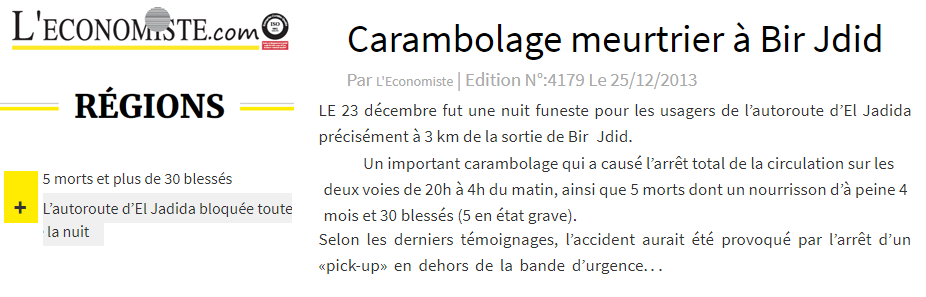
\includegraphics[width=8cm, height=3cm]{img/econ.png}
}
\parbox{5cm}{\caption{ Accident meurtrier sur l’autoroute entre Casablanca et El Jadida au cours de la nuit du 23-24 Décembre 2013 à cause d’un épais brouillard (Source : L’Economiste)}
\label{eco}
}
\end{figure}


Concernant la circulation aérienne, les vols vers un aéroport couvert de brouillard sont souvent reportés ou annulés, menant à des conséquences économiques directes et indirectes.  L’épais brouillard du 20 Janvier 2008 (Cf. Fig. \ref{aujour}) a engendré le
déroutement de 21 avions, devant atterrir à l’aéroport Mohammed V, vers les aéroports de Marrakech, Agadir, Tanger, Fès et Ouarzazate. 
Ainsi, le brouillard a perturbé encore une fois le trafic aérien du royaume le 05 avril 2015 (Cf. Fig. \ref{aujour}). Pour les compagnies aériennes, le déroutement
des avions est synonyme de dépenses plus importantes en kérosène, de prise en charge de passagers, de
remboursements, etc.\\
\begin{figure}[!h]
\parbox{9cm}{
\centering
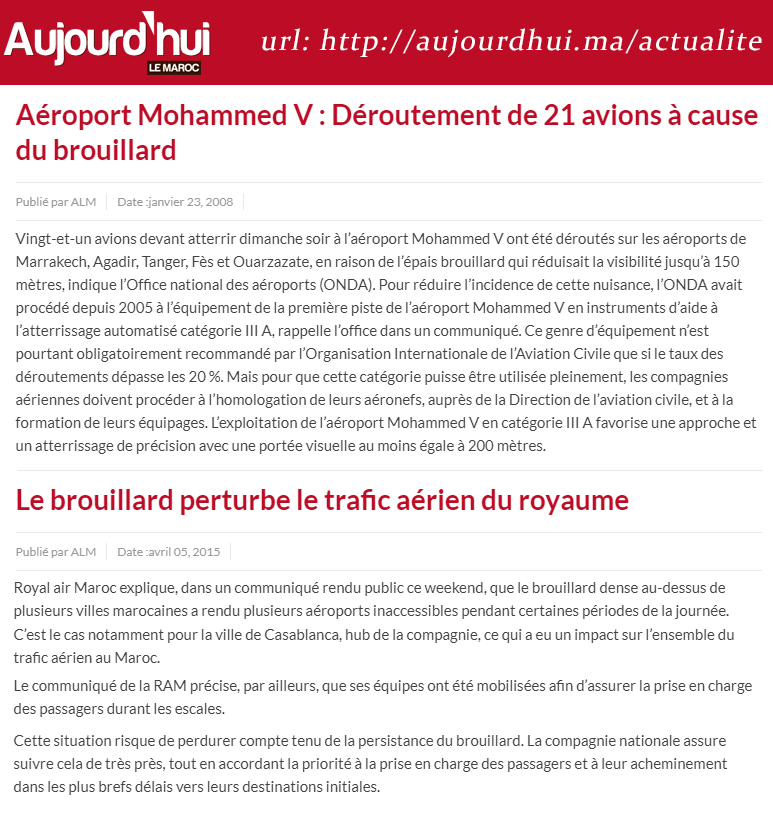
\includegraphics[width=8cm, height=8.2cm]{img/aujourd.png}
}
\parbox{5cm}{
\caption{ Exemples des perturbation d'aéroports du Royaume à cause du brouillard (Source: Aujourd’hui Le Maroc)}
\label{aujour}
}
\end{figure}

À travers ce qui précède, Il s'avère ainsi qu'une bonne prévision de la visibilité horizontale sera d'un grand apport pour les prévisionnistes météorologiques; ce qui réduira en conséquence les impacts néfastes sur certains secteurs socio-économiques et aidera ainsi à une bonne gestion des transports en condition de basse visibilité.


\newpage
%%%%%%%%%%%%%%%%%%%%%%%%%%%%%%%%%%%%%%%%%%%%%%%%%%%%%%%%%%%%%%%%%%%%%%%
\section{Platformes et algorithmes utilisés pour l'estimation de la visibilité : État des lieux}
%%%%%%%%%%%%%%%%%%%%%%%%%%%%%%%%%%%%%%%%%%%%%%%%%%%%%%%%%%%%%%%%%%%%%%%
Dans la littérature scientifique, plusieurs recherches ont abordé la problématique de la détection et la prévision des basses visibilités selon diverses approches (classification et régression) en utilisant diverses plateformes open-sources.
\cite{gultepe2007} ont indiqué, dans l’article de synthèse des travaux de recherche réalisés sur la
thématique du brouillard, que la prévision des événements de basses visibilités en particulier le
brouillard par les modèles de prévision numérique du temps reste difficile, car ce type de phénomène
météorologique dépend de plusieurs facteurs aux échelles locale et globale. Comme alternative, les
chercheurs se sont penchés sur une autre approche qui consiste à utiliser de nouvelles techniques et
méthodologies statistiques dans le but d’élaborer et de développer des modèles pour aider les prévisionnistes à améliorer la prédiction des événements à visibilité réduite dans les aéroports.\\

\cite{bankert} ont utilisé le logiciel C5.0 et Cubist (https://www.rulequest.com/) sous la plateforme \textit{Scikit-learn} (https://scikit-learn.org/) pour estimer le plafond nuageux sur la côte Ouest des États Unis d’Amérique. Les auteurs ont utilisés les données satellitaires issues du GOES-10 et les ont combiné aux données météorologiques issues du modèle COAMPS ainsi que les observations météorologiques conventionnelles issues des METARs \footnote{Un METAR (METeorological Airport Report) est un rapport d’observation (et non de prévision)
météorologique pour l’aviation.}. Les auteurs ont mis en perspective de leur étude, la détection et la prévision de la visibilité, en particulier celle réduite et qui impacte fortement les divers secteurs de transport. \\

\cite{bartokova2015fog}  ont utilisé la plateforme
\textit{WEKA} (https://www.cs.waikato.ac.nz/ml/weka/downloading.html) pour prévoir l’occurrence de certaines
classes de visibilités réduite.
Les auteurs ont développé un modèle basé sur l'arbre de décision (Decision tree) pour prévoir les
événements de brouillard dans la zone désertique côtière de Dubaï. Les auteurs ont conclu que la
combinaison du système WRF-PAFOG unidimensionnel avec un modèle basé sur l'approche Datamining
donne les meilleures prévisions de brouillard. Dans les premières heures de prévision, les prévisions du
modèle à base de Datamining devraient être utilisées, tandis qu'après cette période, les prévisions du
système unidimensionnel de prévision numérique du temps WRF-PAFOG sont meilleures. Mais, leur
étude était restreinte à un seul site.\\

\cite{bari2015lvp} ont élaboré des modèles de prévision des conditions LVP (combinaison entre
visibilité et plafond nuageux) à l’aéroport Mohamed V, Casablanca, Maroc en utilisant les packages (nnet) sous la plateforme open source R (https://cran.r-project.org/). Les auteurs ont utilisé les
réseaux de neurones basés sur la rétro-propagation résiliente comme algorithme d’apprentissage. La
base de données utilisée lors de cette étude était constituée seulement des données observées issues de
la station synoptique météorologique automatique installée à l’aéroport. Les résultats ont été
satisfaisants à cet aéroport mais aucune recherche postérieure n’a été effectuée à l’échelle nationale
pour tester sa performance sur d’autres sites.\\


\cite{kneringer} ont utilisé la package clm() sous la palteforme R 
pour la mise au point un modèle de régression logistique ordonnée (OLR) afin de prédire les probabilités des catégories de procédures de faible visibilité (LVP pour Low Visibility Procedure) à 
l'aéroport international de Vienne. Il est appliqué aux prévisions de saison froide à l'aéroport international de Vienne pour des délais allant de 30 minutes à 2 heures. Les entrées du modèle développé sont les observations météorologiques standards. Les auteurs ont montré que les scores de probabilité classés par l'OLR sont meilleurs que ceux issus de la prévision humaine. Mais, leur étude était restreinte à un seul site.\\


\cite{zhu} ont utilisé les observations météorologiques standards et horaires à l'aéroport
international d'Urumqi en Chine de 2007 à 2016 pour développer un modèle de prévision de la visibilité
basé sur la régression avec la méthode d'apprentissage « Deep Learning » (la plateforme utilisée n'est pas citée par les auteurs). Les résultats montrent que
l'erreur absolue moyenne de la visibilité dominante est de l’ordre de 706 m. Lorsque la visibilité est en dessous de 1000 m, l'erreur absolue moyenne est de 325 m.\\


\cite{bari2017} ont évalué le potentiel des algorithmes Datamining à détecter séparément le brouillard et les nuages bas ainsi qu'à estimer la visibilité horizontale et le plafond nuageux sur la partie nord-ouest du Maroc. Les auteurs ont utilisé le package XGBoost sous la plateforme open source R. Pour l’estimation de la visibilité horizontale
et la hauteur de la base de nuage, les modèles de régression développés enregistrent des
scores de performance satisfaisants quand les données météorologiques locales sont utilisées contrairement aux configurations où les données satellitaires sont utilisées. Ainsi, les
meilleurs modèles estiment ces paramètres continus avec une erreur absolue moyenne
(MAE) de 675m (resp. 540 m) avec 0.96 (resp. 0.93) de corrélation et 1120 m (resp. 1070
m) comme erreur quadratique moyenne (RMSE) dans le cas de visibilité (resp. hauteur
de la base de nuage). En évaluant la généralisation spatiale, les auteurs ont constaté que les modèles
utilisant des données météorologiques présentent des niveaux de performances stables de
station en station contrairement à ceux utilisant uniquement les données satellitaires. Les auteurs n'ont pas utilisé les données issus des modèles de prévision numérique du temps. De plus, leur étude était axée sur la détection à base d'observations et non la prévision.\\

Ce volet de prévision à partir des sorties du modèle de prévision numérique a été abordée par \cite{bari2018visibility} où il a évalué le potentiel de deux techniques machine learning (XGBoost et Deep Learning) à prédire la visibilité horizontale. La performance des algorithmes développés sous la plateforme \textit{H2O} (http://docs.h2o.ai/h2o/) a été comparée à celle produite par la persistance. Les résultats de cette étude a mis en évidence qu'il est suffisant de développer un seul modèle à la base des données couvrant toute la journée au lieu de développer deux modèles l'un à la base des données du jour et l'autre à la base des données nocturnes. Par contre, le meilleur modèle affiche une faible performance quand la généralisation à travers le temps qui peut être due au fait que l'échantillonnage des données en fichiers d'apprentissage et de test était aléatoire. D'autre part, le meilleur modèle, est celui basé sur XGBoost, affiche un biais de -9m, une erreur absolue moyenne de 1349m et une erreur quadratique moyenne de 2150m associé à un coefficient de corrélation linéaire de 0.87.

%%%%%%%%%%%%%%%%%%%%%%%%%%%%%%%%%%%%%%%%%%%%%%%%%%%%%%%%%%%%%%%%%%%%%%%
\section{Objectifs du Stage et Stratégie suivie}
%%%%%%%%%%%%%%%%%%%%%%%%%%%%%%%%%%%%%%%%%%%%%%%%%%%%%%%%%%%%%%%%%%%%%%%
A l’issue des sections précédentes, on constate clairement le besoin en prévision de la visibilité horizontale sur une grande région. Dans la littérature, diverses plateformes et algorithmes ont été utilisés pour l'estimation de la visibilité à partir des diverses sources de données (observations, satellites et sorties des modèles de prévision numérique du temps). En conséquence, les performances des modèles développés différent d'une étude à une autre. Ainsi, la question qui se pose, quelle est la sensibilité de la performance des modèles développés à ces deux composantes principales ( plateforme et algorithme utilisés). C'est la question à laquelle on essayera de répondre au cours de ce stage et c'est son objectif principal.\\

Pour atteindre cet objectif, certaines méthodes de Datamining seront appliquées aux sorties du modèle de prévision numérique du temps AROME (opérationnel à la direction de la météorologie nationale), sous différentes plateformes open-source pour estimer la visibilité horizontale. Ainsi la base de données utilisé dans ce travail, qui couvre 3 années de données horaires, sera répartie en période d’apprentissage (70\% de notre base de données) et une autre de test (le reste de notre base de données 30\%) pour évaluer la performance des algorithmes développés. Il est 
à noter que pour tirer profit au maximum des données, l'échantillonnage sera fait de telle façon de garantir la représentativité des mois, des heures et des diverses classes de visibilités pour toutes les stations synoptiques utilisés dans les deux fichiers de données (test et apprentissage). \\

Après ce chapitre introductif, la méthodologie suivie pour atteindre les objectifs du stage. Ainsi, une description
succincte des plateformes et des algorithmes retenues pour cette étude seront présenté au cours de le chapitre 2. Le
troisième chapitre est dédié à la phase de préparation des données suivie de la phase de modélisation en chapitre 4. Le cinquième chapitre est dédié à l’évaluation des performances
des algorithmes développés et on terminera ce rapport par un chapitre qui résumera les principales conclusions et éventuelles perspectives.













\newpage
\markboth{}{}
\setcounter{mtc}{10}
\chapter[Méthodologie]{Méthodologie}
\label{Methodologie}

\chapterabstract
{Plusieurs plateformes et algorithmes du Datamining ont été employés dans la littérature scientifique pour estimer la visibilité, comme c'est déjà mentionné dans le chapitre introductif. Pour effectuer notre étude, nous avons choisi 
 5 plateformes open source (\textit{Scikit-learn}, \textit{H2O}, \textit{WEKA}, \textit{Tensorflow} et \textit{Keras}) et 4 algorithmes Datamining (\textit{Random Forest}, \textit{Gradient Boosting Machine}, \textit{eXtreme Gradient Boosting} et \textit{Deep Learning}).
Ce chapitre, est dédié  à la méthodologie adoptée pour atteindre les objectifs du stage. Ainsi, nous présenterons au début les plateformes open source, les bibliothèques et les packages utilisés. Par la suite, nous expliquerons le principe de chaque algorithme et ses spécifications, et nous terminerons par les configurations expérimentales adoptées pour le développement des modèles, ainsi que les outils de diagnostics pour évaluer leur performance.}
\pagestyle{plain}

%%%%%%%%%%%%%%%%%%%%%%%%%%%%%%%%%%%%%%%%%%%%%%%%%%%%%%%%%%%%%%%%%%%%%%%%%%%%%%%%%%%%%%%%%%%%%%%%%%%%%%%%%%
\section{Plateformes open sources utilisées}\label{plref}
%%%%%%%%%%%%%%%%%%%%%%%%%%%%%%%%%%%%%%%%%%%%%%%%%%%%%%%%%%%%%%%%%%%%%%%%%%%%%%%%%%%%%%%%%%%%%%%%%%%%%%%%%%
\subsection{WEKA}\label{defWeka}
\begin{wrapfigure}{l}{0.2\textwidth}
    
\includegraphics[width=0.2\textwidth]{img/wekalogo.png}
\end{wrapfigure}
\textit{WEKA} \footnote{disponible sur le web: www.cs.waikato.ac.nz/ml/weka} (Waikato Environment for Knowledge Analysis) est une plateforme open source développée sous Java, qui offre un ensemble d’outils permettant de traiter et d’analyser des fichiers de données. Une collection des algorithmes d'apprentissage automatique (machine learning) est disponible dans cette plateforme. Elle a été développée à l'Université de Waikato en Nouvelle-Zélande \citep{witten2016data}. \\

Sa version originale a été développée en 1992 à la base d'un mélange entre Tk/Tcl\footnote{Tool Command Language/Tool Kit Tool Command Language.}, du langage C et de Makefile\footnote{C'est un fichier contenant un ensemble de directives utilisé par un outil d'automatisation de compilation pour générer une cible / un objectif.}. En 1997, la décision fut prise de développer une nouvelle fois \textit{WEKA} à partir de zéro en Java, y compris l'implémentation des algorithmes de modélisation. En 2005, \textit{WEKA} reçoit le prix SIGKDD (Data Mining and Knowledge
Discovery Service Award). Une année après, en 2006, Pentaho\footnote{est une solution d'informatique décisionnelle open source entièrement développée en Java.} acquiert une licence exclusive pour utiliser \textit{WEKA} dans sa suite décisionnelle open source (version communautaire et
commerciale).  \\


En plus de l'implémentation d'une large gamme d’algorithmes Datamining, plusieurs avantages distingue cet outil dont nous citons quelques-uns:
\begin{itemize}
\item[\textbullet] \textit{WEKA} est disponible en source libre et est gratuit sous la licence GNU\footnote{C'est une licence qui fixe les conditions légales de distribution d'un logiciel libre du projet GNU.};
\item[\textbullet] Portable car il est entièrement implémenté en Java et donc fonctionne sur quasiment toutes les plateformes modernes, ainsi, que tous les systèmes d'exploitation actuels;
\item[\textbullet] \textit{WEKA} contient une collection complète d'outils de prétraitement de données et de techniques de modélisation ;
\item[\textbullet] Facile à utiliser en raison de l'interface graphique qu'il offre.
\item[\textbullet] \textit{WEKA} supporte plusieurs outils d'exploration de données standards, en particulier des prétraiteurs de données, \textit{clustering} de données, des classificateurs statistiques, des analyseurs de régression, des outils de visualisation, et des outils d'analyse discriminante.
\end{itemize}
Cependant, ce logiciel a certain limites en termes de manipulation des analyses complexe et ainsi de visualisation,
\begin{itemize}
\item[\textbullet] \textit{WEKA} n'est pas capable de faire de l'exploration de données multi-relationnelles ;
\item[\textbullet] Certaines fonctionnalités de cette plateforme ne sont pas facilement manipulables comparativement à un logiciel concurrent. 
\item[\textbullet] \textit{WEKA} GUI (Graphical User Interface) fournit plusieurs panneaux intégrés de 'visualisation', mais ceux-ci sont très limités, car la visualisation en \textit{WEKA} se concentre sur la compréhension du comportement des algorithmes, plutôt que sur les ensembles de données ;
\item[\textbullet] L’interface graphique n’est pas aussi bien documentée ou intuitive.
\end{itemize}


\subsection{H2O} \label{defH2O}
\begin{wrapfigure}{l}{0.1\textwidth}
    
\includegraphics[width=0.1\textwidth]{img/h2ologo.png}
\end{wrapfigure}
\textit{H2O} est une plateforme open source d'apprentissage automatique distribuée en mémoire. Elle est produite par la société H2O.ai\footnote{C'est une société spécialisée dans le domaine d’intelligence artificielle et du machine learning.}. Cette plateforme est dédiée à effectuer des analyses prédictives en utilisant des algorithmes de Machine Learning. Elle prend en charge les algorithmes du statistique et d’apprentissage automatique les plus largement utilisés, notamment \textit{Gradient Boosting Machine}, les modèles linéaires généralisés, \textit{Random Forest}, \textit{eXtreme Gradient Boosting}, \textit{Deep learning}, etc.\\

La société H2O.ai a été lancé en 2011 à Mountain View, en Californie (dans la Silicon Valley). La société s'appelait à l'origine 0xdata, mais elle a changé de nom en 2014 pour correspondre à son produit phare, H2O. La plateforme \textit{H2O} est utilisée par plus de 18 000 organisations dans le monde et est extrêmement populaire dans les communautés R et Python.\\


Les principaux avantages de la plateforme \textit{H2O}: 
\begin{itemize}
\item[\textbullet] \textit{Rapide}, tant à l’installation, qu’à la prise en main que dans ses performances algorithmiques.
\item[\textbullet] \textit{Scalable} (évolutif), offre la possibilité d’exploiter un cluster hadoop\footnote{C'est un framework open source qui repose sur Java il prend en charge le traitement des données volumineuses (Big Data) au sein d'environnements informatiques distribués.} existant ou de monter un cluster h2o dédié.
\item[\textbullet] \textit{H2O} est basé sur java et propose une gestion optimisée de la mémoire. 
\item[\textbullet] manipulable via l’interface web fournie ou via des connecteurs pour les langages d’analyse les plus populaires (R, Python, Java, Scala, Spark)\\
\end{itemize}

Les deux limites de cette plateforme les plus répandues sont:   
\begin{itemize}
\item[\textbullet] \textit{H2O} sous Windows ne supporte pas l'algorithme \textit{xGBoost}.
\item[\textbullet] \textit{H2O} étant une plateforme en mémoire, la taille des données est largement limitée par taille de RAM dont vous disposez. 
\end{itemize}


\subsection{Scikit-learn}\label{defscikit}
\begin{wrapfigure}{l}{0.2\textwidth}
    
\includegraphics[width=0.2\textwidth]{img/scikitlogo.png}
\end{wrapfigure}
\textit{Scikit-learn} est un module Python open source sous BSD License\footnote{Berkeley Software Distribution License} (distribution des logiciels de Berkeley), intégrant une large gamme d’algorithmes d’apprentissage automatique qu'ils soient supervisés et non supervisés. Ce paquet met l'accent sur l'apprentissage automatique aux non-spécialistes utilisant un langage de haut niveau. L'accent est mis sur la facilité d'utilisation, les performances, la documentation et la cohérence des API\footnote{Application Programming Interface} (Interface Applicative de Programmation). Ce qui encourage son utilisation dans les milieux académiques et commerciaux \citep{pedregosa2011scikit}. \\


\textit{Scikit-learn} est un code collaboratif à la base, initié par David Cournapeau (promo 2004 Télécom ParisTech\footnote{C'est une grande école d’ingénieurs publique française, spécialisée dans le domaine des technologies de l'information de la communication.}) en 2006. Et comme un sujet du doctorat de Matthieu Brucher ainsi qu'il a été soutenu par plusieurs autres “Google Summer Code”, et par l'Inria (Institut national de recherche en informatique et en automatique) à partir de 2010.\\

Les API de base ont été définies et une liaison efficace de LibSVM \citep{chang2011libsvm} confère au projet un avantage concurrentiel. En décembre 2011, le premier sprint international a été organisé avec un financement généreux de Google. Aujourd'hui, le projet a largement dépassé l'INRIA pour devenir une plateforme mondiale ouverte \citep{article}.\\

Ce qui distingue cette plateforme est sa popularité, en effet il compte plus de 1308 contributeurs à la date de réalisation de cette étude répartis dans le monde, notamment aux États-Unis et en Australie, et on estime à plus de 300 000, le nombre d’utilisateurs réguliers. Le papier historique publié en 2011 a quant à lui dépassé les 16449 citations dans google scholar. Enfin, \textit{Scikit-learn} est largement diffusé dans le milieu académique (à l’école comme dans les plus grandes universités mondiales, la librairie logicielle est utilisée dans les enseignements de machine learning) et industriel (voir les témoignages de Spotify, Change.org ou encore DataRobot sur le site).\\

Outre sa popularité cet outil est se caractérisée par autres avantages nous citons:
\begin{itemize}
\item[\textbullet] \textit{Scikit-learn} simples et efficaces pour l'exploration et l'analyse de données ;
\item[\textbullet] Accessible à tous et réutilisable dans divers contextes ;
\item[\textbullet] Construit sur NumPy\footnote{C'est une bibliothèque Python, qui prend en charge de grands tableaux multidimensionnels et matrices, ainsi qu’une vaste collection de fonctions mathématiques de haut niveau.}, SciPy\footnote{C'est un projet visant à unifier et fédérer un ensemble de bibliothèques Python à usage scientifique. Scipy utilise les tableaux et matrices du module NumPy.} et matplotlib\footnote{C'est une bibliothèque Python destinée à tracer et visualiser des données sous formes de graphiques.} ;
\item[\textbullet] Open source, utilisable dans le commerce - Licence BSD.\\
\end{itemize}

En d'autre part, nous mentionnons quelques limitations de cette plateforme, comparativement aux concurrents dans le même domaine:
\begin{itemize}
\item[\textbullet] Il ne supporte pas le GPU (Processeur graphique) \footnote{Graphics Processing Unit};
\item[\textbullet] Destiné à l'apprentissage machine, plus que l'apprentissage en profondeur (i.e. Deep learning).
\end{itemize}


\subsection{TensorFlow}\label{defTensor}
\begin{wrapfigure}{l}{0.2\textwidth}
    
\includegraphics[width=0.2\textwidth]{img/tensorlogo.png}
\end{wrapfigure}
\textit{Tensorflow} est une puissante bibliothèque d’apprentissage automatique orientée flux de données (Data flow) créée par l'équipe Google Brain de Google et rendue open source en 2015. Elle est conçue pour être facile à utiliser et largement applicable à la fois pour de problèmes liés aux réseaux numériques et neuronaux, ainsi que d'autres domaines. \textit{Tensorflow} est l'un des outils les plus utilisés en intelligence artificielle dans le domaine de l'apprentissage automatique \citep{wiki:xxx}.\\

Le projet Google Brain\footnote{C'est une équipe de recherche en Deep learning et en intelligence artificielle travaillant chez Google. Formé au début des années 2010, Google Brain associe des recherches ouvertes sur l'apprentissage automatique avec ingénierie des systèmes et des ressources informatiques à l'échelle de Google.} a débuté en 2011 pour explorer les utilisations de réseaux de neurones profonds à très grande échelle, à la fois pour la recherche et pour une utilisation dans les produits de Google. Dans le cadre des premiers travaux de ce projet, l'équipe de Google Brain a construit DistBelief, la première génération évolutive d'apprentissage. Et grâce à l'expérience d'équipe avec DistBelief et d'une compréhension plus complète des propriétés de système souhaitables et des exigences en matière d'apprentissage et d'utilisation de réseaux neuronaux, \textit{Tensorflow} a connu le 11 février 2017, la naissance de la deuxième génération de système Google Brain pour la mise en œuvre et le déploiement de modèles d'apprentissage automatique à grande échelle. En février 2018, Google a annoncé la mise à disposition de TPUs\footnote{Tensor Processing Unit.} (unité de traitement de tenseur) en version bêta sur la plateforme Google Cloud \citep{girija2016tensorflow}.\\


Ce qui encourage les utilisateurs de cette outil est ses avantages représenté ci-dessous:
\begin{itemize}
\item[\textbullet] Open source rapide, flexible, et évolutif pour la recherche et la production ;
\item[\textbullet] Portabilité : \textit{Tensorflow} s'exécute sur des GPUs, CPUs (Unité centrale de traitement)\footnote{ Central Processing Unit } et TPUs, desktops et sur les serveurs. Ainsi, il donne la possibilité de déployer un modèle entraîné sur un mobile en tant que partie de produit, et c'est ainsi qu'il constitue une véritable fonctionnalité de portabilité \citep{softwebsolutions}.
\item[\textbullet] \textit{Tensorflow} disponible pour plusieurs langages : Python, R, C++, Java, C\# etc ;
\end{itemize}



\subsection{Keras}\label{defKeras}
\begin{wrapfigure}{l}{0.2\textwidth}
    
\includegraphics[width=0.2\textwidth]{img/keraslogo.png}
\end{wrapfigure}
\textit{Keras} est une API de réseaux de neurones de haut niveau, écrite en Python. En effet, c'est un framework d’apprentissage en profondeur (deep learning) qui offre un moyen pratique de définir et de former presque tous les types de modèles d’apprentissage en profondeur. \textit{Keras} a été initialement développé pour les chercheurs, dans le but de permettre une expérimentation rapide. Ainsi, il est capable de s'exécuter sur \textit{Tensorflow}, Microsoft Cognitive Toolkit (CNTK) ou Theano \citep{Chollet2018}.\\

\textit{Keras} compte plus de 250 000 utilisateurs individuels à la moitié du 2018 (d'après la documentation de cet outil), allant des chercheurs universitaires aux ingénieurs des startups et des grandes entreprises aux étudiants diplômés et aux amateurs. \textit{Keras} est utilisé chez Google, Netflix, Uber, CERN, Yelp, Square et des centaines de startups travaillant sur un large éventail de problèmes. C'est également un framework populaire sur Kaggle\footnote{le site Web du concours d’apprentissage automatique}, où presque tous les concours récents d’apprentissage en profondeur ont été gagnés avec des modèles \textit{Keras}.\\


Il a été développé dans le cadre des efforts de recherche du projet ONEIROS\footnote{Open-ended Neuro-Electronic Intelligent Robot Operating System.} (Système d’exploitation de robot intelligent neuroélectronique). Son auteur et responsable principal est François Chollet, un ingénieur de Google. Sa première publication a eu lieu le 27 mars 2015.\\

En 2017, l'équipe \textit{Tensorflow} de Google a décidé de prendre en charge \textit{Keras} dans la bibliothèque principale de \textit{Tensorflow}. Puis Microsoft a également ajouté à \textit{Keras} un backend CNTK, disponible à partir de CNTK v2.0.\\

De ce qui suit, nous résumons les avantages de cet API dans les points suivants: 
\begin{itemize}
\item[\textbullet] Open source ;
\item[\textbullet] Permet un prototypage simple et rapide (convivialité, modularité et extensibilité) ;
\item[\textbullet] Prend en charge les réseaux convolutifs et les réseaux récurrents, ainsi que les combinaisons des deux ;
\item[\textbullet] Fonctionne parfaitement sur CPU et GPU ;
\item[\textbullet] \textit{Keras} avait plusieurs backends tels que \textit{Tensorflow}, \textit{CNTK} et \textit{Theano} ;
\item[\textbullet] \textit{Keras} est compatible avec Python.\\
\end{itemize}


Cependant, \textit{Keras} ne gère que les API de haut niveau qui s'exécutent sur un autre moteur ou infrastructure tels que \textit{Tensorflow}, \textit{Theano} ou \textit{CNTK}.\\


Les cinq plateformes, packages et bibliothèques expliqué précédemment sont des outils open-source que nous avons utilisé au cours de ce travail, leurs configurations et la comparaison entre elles sera expliqué respectivement dans le chapitre modélisation \ref{conf_plat} et le chapitre évaluation \ref{comp_plat}. \\

Dans la section suivante, nous allons décrire les principaux algorithmes que nous avons adopté pour cette étude, leur principe, leur spécificité et quelques principaux hyperparamètres propres à chacun d'entre eux. 



%%%%%%%%%%%%%%%%%%%%%%%%%%%%%%%%%%%%%%%%%%%%%%%%%%%%%%%%%%%%%%%%%%%%%%%%%%%%%%%%%%%%%%%%%%%%%%%%%%%
\newpage
\section{Algorithmes Datamining utilisés}\label{algo_used}
%%%%%%%%%%%%%%%%%%%%%%%%%%%%%%%%%%%%%%%%%%%%%%%%%%%%%%%%%%%%%%%%%%%%%%%%%%%%%%%%%%%%%%%%%%%%%%%%%%%
Dans cette section, nous allons décrire brièvement les algorithmes d'apprentissage supervisé adoptés en mettant en exergue les spécificités de chacun. Ainsi, deux grandes classes purement distinctes ont été utilisées :
\begin{itemize}
    \item[\ding{224}] Les algorithmes issus des méthodes ensemblistes basées sur l'agrégation des modèles;
    \item[\ding{224}] L'apprentissage profond (deep learning).
\end{itemize}

Les algorithmes issus des méthodes ensemblistes sont basés sur des stratégies adaptatives (boosting, gradient boosting) ou aléatoires (bagging, random forest) permettant d’améliorer l’ajustement par une combinaison
ou agrégation d’un grand nombre de modèles tout en évitant ou contrôlant le sur-ajustement. \\

Remis en veilleuse depuis le milieu des années 90 au profit d’autres algorithmes  d’apprentissage  machine ou  plutôt  statistique : boosting,  random forest..., les réseaux de neurones connaissent un regain d’intérêt et même un énorme battage médiatique sous l’appellation d’apprentissage profond (deep learning). 

\subsection{Random Forest}
\textit{Random Forest} (RF) \citep{breiman2001random} est un algorithme d'apprentissage automatique de famille des modèles ensemblistes (\textit{Ensemble Methods}) qui suit la technique du \textit{Bagging} \footnote{Bagging est une abréviation de Bootstrap aggregating, sert à faire un échantillonnage de données en des sous ensembles.} \citep{breiman1996bagging} améliorée par l'ajout d'une composante aléatoire. L’objectif est donc de rendre plus indépendants les arbres de l’agrégation en ajoutant du hasard dans le choix des variables qui interviennent dans les modèles. Ses estimateurs de base sont des arbres de décision. Il se charge de sélectionner de manière aléatoire un ensemble d’entités \textit{features} qui sont utilisées pour déterminer la meilleure répartition au niveau de chaque nœud de l’arbre de décision \citep{wang2016estimation}.\\

En termes simples, et vu que nous traitons un cas de régression, \textit{Random Forest} combine un grand ensemble d'arbres de régression, chaque arbre représente un ensemble de conditions ou de restrictions organisées hiérarchiquement et appliquées successivement du racine à la feuille de l'arbre, comme indiqué dans la figure (Cf. Fig.\ref{RF_algo}).

\begin{figure}[!htb]
        \center{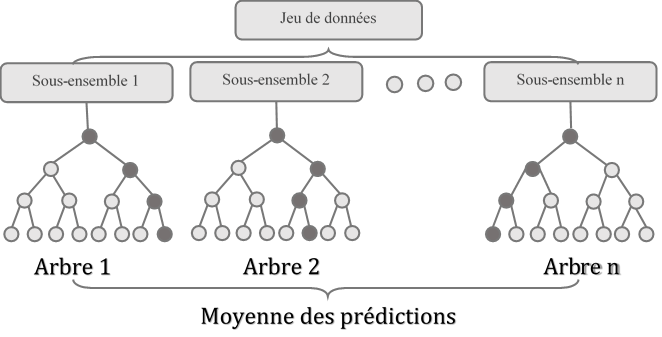
\includegraphics[width=\textwidth]{img/RFalgo.png}}
        \caption{ Random Forest Algorithme}
        \label{RF_algo}
\end{figure}
\begin{tcolorbox}
\footnotesize {
\begin{enumerate}
\item Des sous-ensembles aléatoires sont créés à partir du jeu de données d'origine (Bootstrapping\footnote{Bootstrap aggregating, est une technique d’échantillonnage permette de créer des sous-ensembles d’observations à partir du jeu de données d’origine, avec remplacement.}).
\item sur chaque nœud de l’arbre de décision, un seul ensemble aléatoire d’entités est pris en compte pour déterminer la meilleure répartition.
\item Un modèle d'arbre de décision est entraîné sur chacun des sous-ensembles.
\item La prédiction finale est calculée en faisant la moyenne des prédictions de tous les arbres de décision.
\end{enumerate}
}
\end{tcolorbox}

Cet algorithme a plusieurs hyperparamètres\footnote{hyperparamètre est un paramètre dont la valeur est définie avant le début du processus d'apprentissage.} qui peuvent mener au sur-apprentissage du modèle, ainsi qu'ils joue un rôle primordial dans l'apprentissage du modèle, ces paramètres sont:
\begin{itemize}
    \item[\textbullet] Le nombre d'arbres de régression;
    \item[\textbullet] La profondeur maximale d’un arbre;
    \item[\textbullet] Le nombre de variables d'entrée par noeud.
\end{itemize}



\subsection{Gradient Boosting Machine}
\textit{Gradient Boosting Machine} (GBM) \citep{friedman2002stochastic} est une technique d'apprentissage automatique des problèmes de régression et de classification, qui produit un modèle de prédiction sous la forme d'un ensemble de modèles de prédiction faibles, généralement des arbres de décision. L'idée de gradient boosting est née de l'observation de Leo Breiman en 1997, où il a considéré cette algorithme comme un outil d'optimisation sur une fonction de coût \citep{breiman1997arcing}, des algorithmes de gradient boosting de régression ont ensuite été développés en 2001 par Jerome H. Friedman \citep{friedman2001greedy}.\\

GBM utilise la technique de boosting\footnote{C'est un processus séquentiel dans lequel chaque modèle suivant tente de corriger les erreurs du modèle précédent.}, combinant plusieurs apprenants faibles (\textit{Weak learners}) pour former un apprenant fort (\textit{Strong learner}). Il est à noter que les arbres de régression sont utilisés comme apprenant de base (\textit{base learner}). Le principe de base est de construire une séquence de modèles de sorte que chaque étape, chaque modèle ajouté à la combinaison, apparaisse comme un pas vers une meilleure solution.\\


Cet algorithme suit les étapes suivantes:
\begin{enumerate}
\item Entraîner un simple régresseur linéaire ou un arbre de décision sur les données;
\item Calculer les résidus d'erreur (égale à la valeur cible réelle moins la valeur cible prédite)
$h_1(x)=y-f_1(x)$
\item Entraîner un nouveau modèle sur les résidus d'erreur en tant que variable cible avec les mêmes variables d'entrée $h_1(x)$;
\item Ajouter les résidus prédits aux prédictions précédentes, ce qui signifie la création d'un nouveau modèle, 
$f_2(x)=f_1(x)+h_1(x)$
\item Entraîner un autre modèle sur les résidus qui reste encore. C’est-à-dire $h_2(x)=y-f_2(x)$
\item Et répétez les étapes 2 à 5 jusqu'à ce qu'il commence le sur-apprentissage ou que la somme des résidus devienne constante. Le sur-apprentissage peut être contrôlé en vérifiant systématiquement la précision des données de validation.
$ f_m(x)=f_{(m-1)}(x)+ h_{(m-1)}(x)$ avec $h_{(m-1)}(x)=y- f_{(m-1)}(x)$
\end{enumerate}

\begin{tcolorbox}
\footnotesize {
\begin{enumerate}
\item Initialiser le résultat;
\item Itérer de 1 au nombre total des arbres;
	\begin{enumerate}
		\item Mettre à jour les pondérations pour les cibles en fonction de la série précédente (plus élevées pour celle mal classée);
		\item Ajuster le modèle sur un sous-échantillon de données sélectionné;
		\item Faire des prédictions sur l’ensemble des observations;
		\item Mettre à jour la sortie avec les résultats actuels en tenant compte du taux d’apprentissage;
	\end{enumerate}
\item Renvoyer la sortie finale.\\
\end{enumerate}
}
\end{tcolorbox}
À son tour GBM a quelques hyperparamètres qui requièrent l'optimisation afin d'éviter le sur-apprentissage, ces hyperparamètres sont:
\begin{itemize}
    \item[\textbullet] Le nombre d'arbres de régression;
    \item[\textbullet] La profondeur maximale d’un arbre;
    \item[\textbullet] Le nombre de variables d'entrée par noeud;
    \item[\textbullet] Le taux d'apprentissage lors de la construction du modèle.
\end{itemize}

%%%%%%%%%%%%%%%%%%%%%%%%%%%%%%%%%%%%%%%%%%%%%%%%%%%%%%%%%%%%%%%%%%%%%%%%%%%%%%%%%%%%%%%%%%%%%%%%%%%%%%%%%%%%%%%%%%%%%%%%%%%%%%%
\subsection{eXtreme Gradient Boosting : XGBoost}
\textit{XGBoost} (XGB) signifie \textit{eXtreme Gradient Boosting} est une implémentation open source populaire et efficace de l'algorithme gradient boosting trees, développé par Tianqi Chen\footnote{pour plus d'info: https://tqchen.github.io/} en 2016. \\

Comme nous avons déjà cité dans l'explication de l'algorithme précédent GBM, c'est un algorithme d'apprentissage supervisé qui tente de prédire avec précision une variable cible en combinant les estimations d’un ensemble de modèles plus simples et plus faibles. \\

En revanche, l'algorithme XGB est distingué par sa flexibilité et sa portabilité, en effet il fournit un \textit{Tree Boosting} parallélisé qui résout de nombreux problèmes de science de données d'une manière rapide et précise. Notamment, il a démontré son efficacité dans plusieurs compétitions d’apprentissage automatique, car il gère variété de types de données, de relations et de distributions, ainsi qu'un grand nombre de ses hyperparamètres pouvant être réglés et optimisés pour des améliorations au niveau d'apprentissage \citep{chen2016xgboost}.\\


Un estimateur $\phi $ additif à K arbre, de l'algorithme XGB, se formalise pour des entrées $(x_i, y_i)\in R^m\times R$ par l’équation \ref{eq1}.
\begin{equation}\label{eq1}
    \widetilde{y_l}=\phi (x_i)=\sum_{i=1}^{N}f_k(x_i), f_k \in \mathcal{F}
\end{equation}
Où $\widetilde{y_l}$ est l’estimation de $y_i$ et $\mathcal{F}= f(x) = \omega_{q(x)} (q:R^m \xrightarrow{}T, \omega \in R^T$ est l’espace des représentants des arbres de décisions et de régressions (CART). T et $\omega_i $ désignent respectivement le nombre de feuilles de l’arbre et la valeur associée aux points de la $i^{ème}$ feuille. $q$ désigne la fonction de structure de l’arbre qui a un échantillon $x_i$ associe l’indice de la feuille à laquelle il appartient. Afin d’obtenir les fonctions utilisés dans le modèle, on cherche à minimiser la fonction objectif régularisée $\mathcal{L}$ donnée par l’équation \ref{eq2}.
\begin{equation}\label{eq2}
    \mathcal{L}(\phi) = \sum_i l(\widetilde{y_l},y_i)+\sum_{k}\Omega(f_k)
\end{equation}

où $\Omega(f_k) = \gamma T +\lambda \| \omega \|_2 + \alpha \| \omega \|_1$\\

$l$ Désigne une fonction de perte convexe et différentiable. Cette minimisation se fait de manière
gloutonne en améliorant l’estimateur par l’ajout d’un arbre à chaque itération. A l’itération t, on cherche
à ajouter un nouvel arbre $f_t$ qui améliore les estimations des modèles, i.e. qui minimise la fonction
objectif $\mathcal{L}_t$ à l’instant t donnée par l’équation \ref{eq3}, où $\widetilde{y}_{l}^{t-1}$ est l’estimation de $y_i$ à l’issue de l’itération
précédente.
\begin{equation}\label{eq3}
    \mathcal{L}_t = \sum_{i} l(y_i , \widetilde{y}_{l}^{t-1}) + f_{t}(x_i) + \Omega (f_t)
\end{equation}\\

En utilisant une approximation au deuxième ordre de $\mathcal{L}_t$et en éliminant les termes constants, on obtient la nouvelle fonction objectif $\widetilde{\mathcal{L}_t}$ donnée par l’équation \ref{eq4}.
\begin{equation}\label{eq4}
    \widetilde{\mathcal{L}_t} = \sum_{i}[g_{i}f_{t}(x_{i} + \frac{1}{2} h_{i}f_{t}^2(x_i)] + \Omega (f_t)
\end{equation}

où $ g_i = \partial_{\widetilde{y}_{l}^{t-1}} l(y_{i}, \widetilde{y}_{l}^{t-1}) $ et $ h_i = \partial_{\widetilde{y}_{l}^{t-1}}^2 l(y_{i}, \widetilde{y}_{l}^{t-1}) $\\

En plus du terme de régularisation $\Omega$ plusieurs autres outils permettent d’empêcher l’occurrence de surapprentissage.
Parmi ces derniers nous avons considérés dans notre étude les suivants :
\begin{itemize}
    \item [\textbullet] La profondeur maximale d’un arbre ;
    \item [\textbullet] Un facteur de rétrécissement $\eta$ appliqué aux poids w des arbres les plus récents ;
    \item [\textbullet] Un sous-échantillonnage aléatoire des colonnes au niveau de chaque arbre ;
    \item [\textbullet] Taux de la réduction des écarts.\\
\end{itemize}

Les trois algorithmes décrits précédemment (RF, GBM, XGB) sont de famille ensembliste, ils sont basés principalement sur les arbres de régression, ces méthodes font générer plusieurs arbres qui sont ensuite combinées pour produire une prédiction finale. En effet, la combinaison d'un grand nombre d'arbres peut souvent entraîner des améliorations considérables sur la précision et la performance des prévisions.\\

Par ailleurs, la quatrième algorithme de cette étude est \textit{Deep learning} qui se base particulièrement sur des neurones artificielles. Dans ce qui suit nous détaillons ce genre d'algorithme.  
%%%%%%%%%%%%%%%%%%%%%%%%%%%%%%%%%%%%%%%%%%%%%%%%%%%%%%%%%%%%%%%%%%%%%%%%%%%%%%%%%%%%%%%%%%%%%%%%%%%%%%%%%%%%%%%%%%%%%
\subsection{Réseau de Neurone Artificiel}
L’\textit{Intelligence Artificielle}, branche de l’Informatique fondamentale s’est
développée avec pour objectif la simulation des comportements du cerveau
humain. Les premières tentatives de modélisation du cerveau sont anciennes
et précèdent même l’ère informatique. C’est en 1943 que Mc Culloch (neuro-
physiologiste) et Pitts (logicien) ont proposé les premières notions de \textit{neurone
formel}. Ce concept fut ensuite mis en réseau avec une couche d’entrée et une
sortie par Rosenblatt en 1959 pour simuler le fonctionnement rétinien et tacher
de reconnaître des formes. C’est l’origine du \textit{perceptron}. Cette approche dite 
\textit{connexioniste} a atteint ses limites technologiques, compte tenu de la puissance 
de calcul de l’époque, mais aussi théoriques au début des années 70.\\

Au début des années 80 ont permis de relancer l’approche connexioniste. Celle-
ci a connu au début des années 90 un développement considérable si l’on
considère le nombre de publications et de congrès qui lui ont été consacrés
mais aussi les domaines d’applications très divers où elle apparaît. Ainsi, 
les réseaux de neurones connaissent un regain d’intérêt et même un énorme battage médiatique sous l’appellation d’apprentissage profond (\textit{deep learning}).\\

Les réseaux de neurones artificiels consistent en des modèles plus ou moins
inspirés du fonctionnement cérébral de l’être humain en se basant principalement
sur le concept de neurone biologique (Cf. Fig. \ref{neuron_bio}), qui se compose de :
noyau\footnote{intègre les signaux entrants et génère un signal sortant vers axone}, 
axone\footnote{transmet des signaux électriques aux dendrites d'une autre cellule à l'aide de synapses
}, 
dendrites et 
synapse\footnote{recueillir des signaux électriques.}. Les neurones sont faits pour transmettre des informations.\\

\begin{figure}[!htb]
        \center{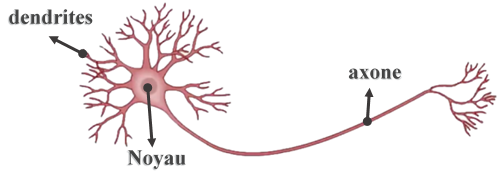
\includegraphics[width=10cm]{img/neuronbio.png}}
        \caption{ Neurone Biologique}
        \label{neuron_bio}
\end{figure}


Un neurone artificiel ou un perceptron en termes simples, calcule une « somme pondérée » de son entrée, ajoute un biais et décide ensuite s’il doit être faire une telle action ou non (Cf. Fig. \ref{neuron_art}).
Par exemple un neurone $$y=\sum(poids*entrées)+biais$$

\begin{figure}[!htb]
        \center{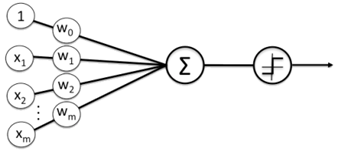
\includegraphics[width=10cm]{img/neuronartif.png}}
        \caption{Neurone Artificiel}
        \label{neuron_art}
\end{figure}

\subsubsection{Fonctions d’activation}\label{fun_activ}
Les fonctions d'activation prennent comme paramètres la somme pondérée des entrées ainsi que le seuil d’activation. Elle calcule la valeur de sortie à partir du résultat de la fonction de combinaison : $S_j=f(v_j)$ avec $S_j$ est la valeur de sortie, $f$ est la fonction d’activation, et $v_j$ est la fonction de transition.

\paragraph*{Fonction à seuil « Step function »}
\begin{wrapfigure}{r}{0.2\textwidth}
    \vspace{-1 cm}
    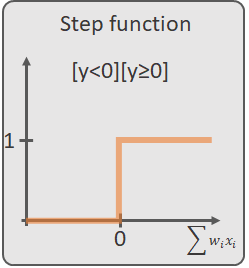
\includegraphics[width=0.2\textwidth]{img/stepfunc.png}
    \vspace{-1 cm}
\end{wrapfigure}
C’est une fonction d’activation basée sur un seuil. Si la valeur de $y$ dépasse une certaine valeur, le neurone est activé. L’inconvénient de ce type des fonctions est qu'elles ne prennent pas des valeurs intermédiaires. Cependant, elles fonctionnent parfaitement pour les problèmes qui ont des sorties binaires. 


\paragraph*{Fonction Linéaire}
\begin{wrapfigure}{r}{0.2\textwidth}
    \vspace{-1 cm}
    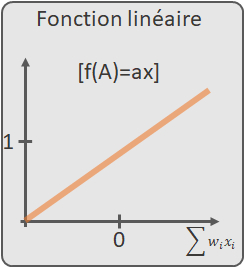
\includegraphics[width=0.2\textwidth]{img/linfunc.png}
    \vspace{-1 cm}
\end{wrapfigure}
C’est une fonction en ligne droite où l'activation est proportionnelle à l'entrée (qui est la somme pondérée du neurone). 
De cette façon, cela donne une gamme d'activations qui n'est pas forcément binaire comme dans le cas précédant de \textit{step function}.
L'inconvénient de cette fonction est que la dérivée est une constante. Peu importe le nombre de couches dont nous disposons, si toutes sont de nature linéaire, la fonction d'activation finale de la dernière couche n'est rien d'autre qu'une fonction linéaire de l'entrée de la première couche ! Cela signifie que ces couches peuvent être remplacées par une seule couche. Alors nous avons besoin d’une fonction qui nous donne la possibilité d'empiler des couches.


\paragraph*{Fonction sigmoïde}
\begin{wrapfigure}{r}{0.2\textwidth}
    \vspace{-1 cm}
    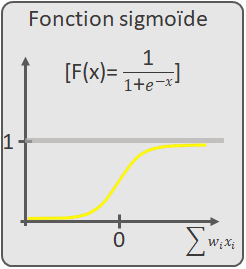
\includegraphics[width=0.2\textwidth]{img/segfunc.png}
    \vspace{-1 cm}
\end{wrapfigure}
C’est une fonction de nature non linéaire qui permet d'empiler des couches. Ainsi, elle donnera une activation analogique contrairement à la fonction à seuil. Il est à noter que toute modification mineure des valeurs de X dans cette région au voisinage de 0 entraînera une modification significative des valeurs de Y. Ce qui distingue cette fonction est que, contrairement à la fonction linéaire, la sortie de la fonction d'activation sera toujours dans la plage (0,1) par rapport à ($-\infty, \infty$) de la fonction linéaire. La fonction sigmoïde est l’une des fonctions d’activation les plus utilisées. 

\paragraph*{Fonction tanh}
\begin{wrapfigure}{r}{0.2\textwidth}
    \vspace{-1 cm}
    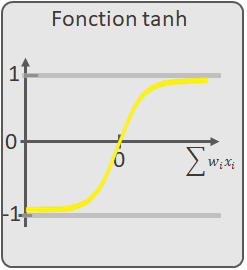
\includegraphics[width=0.2\textwidth]{img/tanhfunc.png}
    \vspace{-1 cm}
\end{wrapfigure}
Cette fonction ressemble à la fonction Sigmoïde. La différence avec la fonction Sigmoïde est que la fonction Tanh produit un résultat compris entre -1 et 1. La fonction Tanh est en terme général préférable à la fonction Sigmoïde car elle est centrée sur zéro. Les grandes entrées négatives tendent vers -1 et les grandes entrées positives tendent vers 1. Mis à part cet avantage, la fonction Tanh possède les mêmes autres inconvénients que la fonction Sigmoïde.

\paragraph*{Fonction ReLu « rectified linear unit »}
\begin{wrapfigure}{r}{0.2\textwidth}
    \vspace{-1 cm}
    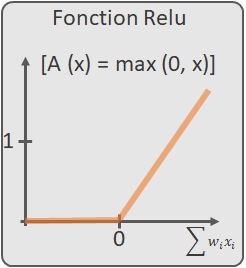
\includegraphics[width=0.2\textwidth]{img/relufunc.png}
\end{wrapfigure}
Pour résoudre le problème de saturation des deux fonctions précédentes (Sigmoïde et Tanh) il existe la fonction ReLU (Unité de Rectification Linéaire). Cette fonction est la plus utilisée. La fonction ReLU est interprétée par la formule: $f(x) = max(0, x)$. Si l'entrée est négative la sortie est 0 et si elle est négative alors la sortie est x. Cette fonction d'activation augmente considérablement la convergence du réseau et ne sature pas.
Mais la fonction ReLU n'est pas parfaite. Si la valeur d'entrée est négative, le neurone reste inactif, ainsi les poids ne sont pas mis à jour et le réseau n’apprend pas. ReLu est de nature non linéaire, cela signifie qu'elle nous donne la possibilité d'empiler des couches. La plage de ReLu est [0, $\infty$).


\subsubsection{Perceptron Multicouche MLP}
Le Perceptron Multicouche (MLP) est un des réseaux de neurones les plus utilisés pour des problèmes d’approximation, de classification et de prédiction. Il est habituellement constitué de trois ou plusieurs couches de neurones totalement connectées : une couche d’entrées, une de sortie et une ou plusieurs couches cachées.\\ 

Dans le cas général, un Perceptron multicouche peut posséder un nombre de couches quelconque et un nombre de neurones par couche également quelconque \citep{parizeau2004perceptron}. La taille (définie par le nombre de nœuds dans chaque couche cachée) optimale du réseau dépend de la complexité du problème et l’architecture choisie. Ce type de réseau fait partie de la famille des réseaux non bouclés (Feedforward network), c’est-à-dire qu’en mode normal d’utilisation, l’information se propage dans un sens unique, des entrées vers les sorties sans aucune rétroaction.\\

La figure \ref{MLP_fig} explicite l’exemple d’un réseau contenant une couche d’entrée, deux couches cachées et une couche de sortie. La couche d’entrée représente une couche virtuelle associée aux entrées du système, elle est composée de 3 paramètres et elle ne contient pas de neurone. Par contre, on distingue 3 neurones dans la première couche cachée, 4 neurones dans la deuxième et 2 neurones dans la couche de sortie. Les sorties des neurones
de la dernière couche correspondent aux sorties du réseau.

\begin{figure}[!htb]
        \center{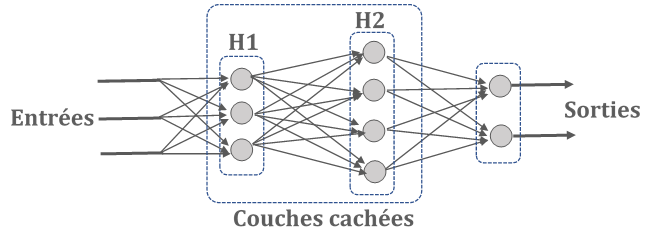
\includegraphics[width=\linewidth]{img/mlp.png}}
        \caption{Schéma d'un perceptron multicouche}
        \label{MLP_fig}
\end{figure}

\subsubsection{Apprentissage du MLP}

L’apprentissage du réseau de neurones a pour finalité que ce réseau donne les bonnes sorties sur un ensemble d’exemples, appelé \textit{ensemble de test}. Pour cela, on va utiliser un ensemble d’exemples sur lequel le réseau va s’entraîner et apprendre. Cet ensemble s’appelle l’\textit{ensemble d’apprentissage}. Les exemples de l’ensemble de test n’appartiennent pas à l’ensemble d’apprentissage. Ainsi, avec cette méthode basée sur la distinction entre l’ensemble d’apprentissage et celui du test, le réseau de neurones doit être capable de généralisation. Dans la plupart des architectures, l’apprentissage se traduit par un changement dans la valeur des poids qui relient les neurones d’une couche à l’autre.\\

Dans notre étude, nous avons utilisé un apprentissage de type \textit{supervisé} qui a pour principe d’ajuster les poids à la base de la comparaison des sorties connues aux sorties prévues par le réseau de telle façon que l’écart entre les deux soit minimal. Par conséquent, trouver les poids optimums pour le réseau de neurones est équivaut à la recherche du minimum global de la fonction coût $E$. Un ensemble de règles bien définies permettant de réaliser un tel processus d’adaptation des poids constitue ce qu’on appelle l’\textit{algorithme d’apprentissage du réseau} et l'approche adoptée au cours de ce travail est la \textit{rétro-propagation}.\\

En fait, la rétro-propagation permet la recherche d’un minimum local de la fonction d’erreur $E$ à travers la mise à jour des poids du réseau. Cette mise à jour se fait par plusieurs méthodes, la plus utilisée étant la descente du gradient (traduction libre de Gradient descent), elle consiste à retrancher le gradient de la fonction d’erreur multiplié par un taux fixe de la valeur du poids de l’itération qui précède. Le taux $\eta$ étant de sens opposé par rapport au gradient de la fonction d’erreur \citep{gunther2010neuralnet}.

Ainsi, les poids sont ajustés par la règle suivante :
            \begin{equation}
            \Delta\omega_{ij}^{(t)}=\omega_{ij}^{(t+1)}-\omega_{ij}^{(t)}=-\eta
            \frac{\partial E^{(t)}}{\partial \omega_{ij}^{(t)}}
            \end{equation}
            où $t$ est l'indice de l'itération.\\

Afin de rendre l'apprentissage plus stable, un \emph{moment} est ajouté à la formule précédente traduisant l'influence du poids de l'itération précédente :
            \begin{equation}
            \Delta\omega_{ij}^{(t)}= -\omega_{ij}^{(t)}=-\eta \frac{\partial
            E^{(t)}}{\partial \omega_{ij}^{(t)}} + \mu \Delta\omega_{ij}^{(t-1)}
            \end{equation}

%%%%%%%%%%%%%%%%%%%%%%%%%%%%%%%%%%%%%%%%%%%%%%%%%%%%%%%%%%%%%%%%%%%%%%%%%%%%%%%%%%%%%%%%%%%%%%%%%%%
\section{Configurations expérimentales}\label{config}
%%%%%%%%%%%%%%%%%%%%%%%%%%%%%%%%%%%%%%%%%%%%%%%%%%%%%%%%%%%%%%%%%%%%%%%%%%%%%%%%%%%%%%%%%%%%%%%%%%%
\subsection{Par plateforme et par algorithme}\label{config_pl_algo}
L'objectif principal de notre étude est d'évaluer la sensibilité de la performance des modèles développés à la plateforme et l'algorithme utilisés dans le cas d'un problème de régression, et qui traite l'estimation de la visibilité horizontale à partir des sorties d'un modèle de prévision numérique du temps. Pour atteindre cet objectif, nous avons effectué plusieurs configurations expérimentales combinant les plateformes open source (\textit{Scikit-learn}, \textit{H2O}, \textit{WEKA}, \textit{Tensorflow} et \textit{Keras}) et les algorithmes d'apprentissage automatique adoptés (Random Forest, Gradient Boosting Machine, eXtreme Gradient Boosting et Deep Learning).\\

Dans la première phase de modélisation, les modèles ont été développé à la base des configurations par défaut implémenté dans chaque algorithme et chaque plateforme. Autrement dit, les hyperparamètres de la configuration de base ont été utilisés. Dans la suite, on résumera ces paramètres par algorithme pour chaque plateforme.\\


\begin{itemize}
    \item[\ding{233}]\textbf{Random Forest}\\%%%%%%%%%%%%%%%%%%%%%%%%%%%%%%%%%%%%%%%%%%%%%%%%%%%%%%%%%%%%%%%%%%%%%%%%%%%%%%%%%%%%%
    
    Le tableau  \ref{tab:RF} récapitule les principaux hyperparamètres adoptés pour l'algorithme \textit{Random Forest} pour les plateformes retenues. Il est à noter que l'appellation des hyperparamètres diffèrent d'une plateforme à une autre. Ceci a constitué un challenge pour la mise en place de notre étude. Certains paramètres sont décrits brièvement comme note de bas du tableau. Il est à noter que cet algorithme a été utilisé sur trois plateformes : \textit{Scikit-learn}, \textit{H2O} et \textit{WEKA}.\\
\\
\\

        \begin{table}[h!]
        \centering
        \begin{threeparttable}[t]
        \begin{tabular}{|c||p{8cm}p{2cm}|}
        \hline
        plateforme & \multicolumn{2}{|c|}{Valeur des hyperparamètres}  \\ \hline
        \multirow{6}{*}{Scikit-learn} 
        & n\_estimators & 10  \\
        & min\_samples\_split & 2  \\ 
        & min\_samples\_leaf & 1 \\
        & max\_features & auto\tnote{1}\\
        & max\_depth & None\tnote{2}\\
        & bootstrap & True\tnote{3}\\
         \hline
        \multirow{4}{*}{H2O} 
        & ntrees & 50  \\
        & max\_depth & 20\\
        & min\_rows & 1  \\ 
        & mtries & -1\tnote{4}\\
         \hline
        \multirow{3}{*}{WEKA} 
        & numEtirations & 100  \\
        & maxDepth & 0\\
        & numFeatures & 0  \\ 
         \hline
        \end{tabular}
        \footnotesize{
        \begin{tablenotes}
              \item[1] max\_features=n\_features; 
              \item[2] nœuds sont développés jusqu'à ce que toutes les feuilles soient pures ou jusqu'à ce que toutes les feuilles contiennent moins de min\_samples\_split;
              \item[3]si False, le jeu de données est utilisé complètement pour construire chaque arbre;
              \item[4]le nombre de variable est p / 3 pour la régression (où p est le nombre de prédicteurs).
        \end{tablenotes}
        }
       \end{threeparttable}
        \caption{Les hyperparamètres de RF choisis par défaut pour chaque plateforme}
        \label{tab:RF}
        \end{table}

    \item[\ding{233}]\textbf{Gradient Boosting Machine}\\%%%%%%%%%%%%%%%%%%%%%%%%%%%%%%%%%%%%%%%%%%%%%%%%%%%%%%%%%%%%%%%%%%%%%%%%%
    
    Le tableau  \ref{tab:GBM} récapitule les principaux hyperparamètres adoptés pour l'algorithme \textit{Gradient Boosting Machine} pour les plateformes retenues : \textit{Scikit-learn} et \textit{H2O}.\\
        \begin{table}[h!]
        \centering
        \begin{tabular}{|c||p{8cm}p{2cm}|}
        \hline
        plateforme & \multicolumn{2}{|c|}{Valeur des hyperparamètres}  \\ \hline
        \multirow{6}{*}{Scikit-learn} 
        & n\_estimators & 100  \\
        & min\_samples\_split & 2  \\ 
        & min\_samples\_leaf & 1 \\
        & max\_features & None\\
        & max\_depth & 3\\
        & learning\_rate  & 0.1\\
         \hline
        \multirow{4}{*}{H2O} 
        & ntrees & 50  \\
        & max\_depth & 5\\
        & min\_rows & 10  \\ 
        & learn\_rate & 0.1 \\
        & sample\_rate & 1 \\
         \hline
        \end{tabular}
        \caption{Les hyperparamètres de GBM choisis par défaut pour chaque plateforme}
        \label{tab:GBM}
        \end{table}
        
    \item[\ding{233}]\textbf{eXtreme Gradient Boosting}\\%%%%%%%%%%%%%%%%%%%%%%%%%%%%%%%%%%%%%%%%%%%%%%%%%%%%%%%%%%%%%%%%%%%%%%%%%%
        Le tableau  \ref{tab:GBM} récapitule les principaux hyperparamètres adoptés pour l'algorithme \textit{eXtreme Gradient Boosting} pour les plateformes retenues : \textit{Scikit-learn} et \textit{H2O}.\\
        \begin{table}[h!]
        \centering
        \begin{tabular}{|c||p{8cm}p{2cm}|}
        \hline
        plateforme & \multicolumn{2}{|c|}{Valeur des hyperparamètres}  \\ \hline
        \multirow{5}{*}{Scikit-learn} 
        & n\_estimators & 100  \\
        & gamma & 0 \\ 
        & colsample\_bytree & 3 \\
        & learning\_rate & 0.1\\
        & max\_depth & 3\\
         \hline
        \multirow{3}{*}{H2O} 
        & ntrees &   50 \\
        & max\_depth & 6\\
        & min\_rows &  1 \\ 
         \hline
        \end{tabular}
        \caption{Les hyperparamètres de XGB choisis par défaut pour chaque plateforme}
        \label{tab:XGB}
        \end{table}

    \item[\ding{233}]\textbf{Deep Learning}\\%%%%%%%%%%%%%%%%%%%%%%%%%%%%%%%%%%%%%%%%%%%%%%%%%%%%%%%%%%%%%%%%%%%%%%%%%%%%%%%%%%%%%
Le tableau  \ref{tab:DL} récapitule les principaux hyperparamètres adoptés pour l'algorithme Deep Learning pour les plateformes retenues : \textit{Scikit-learn}, \textit{H2O}, \textit{WEKA} et \textit{Keras}.

        \begin{table}[h!]
        \centering
        \begin{threeparttable}[t]
        \begin{tabular}{|c||p{8cm}p{1.5cm}|}
        \hline
        plateforme & \multicolumn{2}{|c|}{Valeur des hyperparamètres}  \\ \hline
        \multirow{4}{*}{Scikit-learn} 
        & activation & relu  \\
        & hidden\_layer\_sizes & 100  \\
        & max\_iter & 200 \\
        & num hidden layer & 1 \\
         \hline
        \multirow{3}{*}{H2O} 
        & activation & Rec\\
        & size hidden layers & 200  \\
        & num hidden layers & 2  \\ 
         \hline
        \multirow{3}{*}{WEKA} 
        & hidden\_layer & a\tnote{1}  \\
        & learning\_rate & 0.3 \\
        & momentum & 0.2  \\ 
         \hline
        \multirow{3}{*}{KERAS} 
        &Cet outil n'a pas de configuration par défaut pour le deep learning. Pour spécifier un perceptron simple, il faut ajouter une couche qui relie directement la couche d’entrée (nombre de neurones = nombre de variables prédictives) avec la couche de sortie, tout en précisant une fonction d’activation.&\\
         \hline
        \end{tabular}
        \footnotesize{
            \begin{tablenotes}
                  \item[1]  a= (attributs + classes) / 2, i= attributs, o= classes , t= attributs + classes."
            \end{tablenotes}
        }
        \end{threeparttable}
        \caption{Les hyperparamètres de DL choisis par défaut pour chaque plateforme}
        \label{tab:DL}
        \end{table}
        
\end{itemize}





\newpage

\subsection{Optimisation des hyperparamètres}\label{opt_algo}
Vu que les algorithmes utilisés dans cette étude ont un nombre très important des hyperparamètres, alors leur optimisation est nécessaire car elle nous aide à trouver le modèle optimal minimisant une fonction de perte prédéfinie sur des données de test.\\

Dans ce travail nous avons utilisé 2 approches d'optimisation des hyperparamètres:\\
\begin{itemize}
    \item [\ding{109}] \textbf{Grid search:}\\ 
    
    C'est une méthode d’optimisation (hyperparameter optimization) qui va nous permettre de tester une série de paramètres et de comparer les performances pour en déduire le meilleur paramétrage. Ainsi, pour chaque paramètre, on détermine un ensemble de valeurs que l’on souhaite tester. Par exemple, dans le cas d’un Random Forest on pourrait tester :
    \begin{itemize}
        \item[\textbullet] Nombre d’arbres : \{ 10, 20, 30 \}
        \item[\textbullet] Nombre de variables sélectionnées : \{ 2, 3, 4, 5 \}\\
    \end{itemize}
    
Le Grid Search croise simplement chacune de ces hypothèses et va créer un modèle pour chaque combinaison de paramètres. Dans notre exemple nous aurons $3 \times 4 = 12$ modèles à construire. Grid Search a aussi ses limites puisque c’est l'utilisateur qui définit à l’avance les paramètres qu'il veut tester.\\ 
    \item [\ding{109}] \textbf{Random search:}\\ 
    
    C'est une technique dans laquelle des combinaisons aléatoires des hyperparamètres sont utilisées pour trouver la meilleure solution d'un modèle développé.\\
\end{itemize}

Ces approches d'optimisation sont utilisées par plateforme et par algorithme pour trouver le meilleur modèle. 

%%%%%%%%%%%%%%%%%%%%%%%%%%%%%%%%%%%%%%%%%%%%%%%%%%%%%%
\subsection{Analyse croisée par plateforme et par algorithme} \label{sec:ana-cross}
L'un des objectifs principaux de ce stage est d'évaluer la sensibilité de la performance du modèle développé à la plateforme open source et à l'algorithme Datamining choisis. Pour atteindre cet objectif, nous allons intégrer les hyperparamètres optimums obtenus soit par Grid search soit par Random search pour une plateforme donnée, dans le même algorithme mais pour une autre plateforme.\\

Par exemple si l'algorithme Random Forest dans la plateforme \textit{Scikit-learn} nous donne un erreur minimal avec un nombre d'arbres égale à 20, nous essayerons de faire appel au même algorithme (Random Forest) dans \textit{H2O} et \textit{WEKA} avec nombre d'arbre égale à 20, et d'évaluer l'impact sur la performance du modèle développé.\\

Tenant compte du fait que l'appellation des hyperparamètres diffèrent d'une plateforme à une autre, nous avons limité notre analyse croisée par plateforme et par algorithme, aux hyperparamètres dont les équivalents existent dans les deux plateformes comparées. Par exemple: l'hyperparamètre  \textbf{n\_estimators} qui indique le nombre d'arbre pour Random Forest en Scikit-learn, son équivalent en H2O est \textbf{ntrees} et dans \textit{WEKA} c'est \textbf{numEtirations}. Pour les autres hyperparamètres, ils ont gardé leurs valeurs par défaut. 


%%%%%%%%%%%%%%%%%%%%%%%%%%%%%%%%%%%%%%%%%%%%%%%%%%%%%%%%%%%%%%%%%%%%%%%%%%%%%%%%%%%%%%%%%%%%%%%%%%%
\section{Outils de Diagnostics }
%%%%%%%%%%%%%%%%%%%%%%%%%%%%%%%%%%%%%%%%%%%%%%%%%%%%%%%%%%%%%%%%%%%%%%%%%%%%%%%%%%%%%%%%%%%%%%%%%%%
Tenant compte de l'intérêt émergent à l'utilisation du Datamining dans pas mal de secteurs socio-économiques, le nombre d’outils d’exploration de données disponibles ne cesse de croître. Par conséquent, la concurrence entre les développeurs de logiciels d'exploration de données augmente également et le choix de l'outil le plus approprié devient de plus en plus difficile. Ainsi, la comparaison des outils d'exploration de données devient nécessaire même si elle n'est pas évidente. Au cours de cette section, nous allons expliciter certains critères de comparaison des plateformes retenues ainsi que les critères d'évaluation de la performance des algorithmes Datamining utilisés.

\subsection{Critères de comparaison des plateformes utilisées}
La comparaison entre plateformes open sources n'est pas évidente car elle fait appel à plusieurs critères (structures de données, les algorithmes implémentés, capacités de visualisation, langages de programmation, options d'importation et d'exportation, etc.). Pour ce faire, on s'est focalisé sur les critères suivants et qui ont été adoptés par \cite{chen2007survey} : les caractéristiques générales, la gestion des données, leur fonctionnalité et le mode d'utilisation.\\

\begin{itemize}
    \item[\ding{233}]\textbf{ Les caractéristiques générales :}\\
    Les caractéristiques générales considérées de la plateforme comprennent le nom de la plateforme, l'architecture, le système d’exploitation et le langage de programmation. En ce qui concerne l’architecture, les outils du Datamining peuvent être subdivisées en architecture autonome (standalone) et/ou architecture client /serveur. Le premier type ne nécessite aucun logiciel autre que le système d’exploitation, contrairement à l’architecture client / serveur. L'une des tendances émergentes est le nombre croissant d'interfaces Web fournissant l'exploration de données. Par conséquent, une architecture de service \textit{cloud} basée sur le Web sera également incluse en tant que valeur possible pour l'architecture des plateformes.\\
    
    \item[\ding{233}] \textbf{La gestion des données :}\\
    Tenant compte de la diversité des types de données, il est impossible de trouver un outil Datamining qui exploite toute sorte de format de données.
    Les outils du Datamining nécessite une intégration avec des systèmes de gestion de base de données (database systems) ou avec des entrepôts de données (data warehouse) pour la sélection des données, leur prétraitement et transformation, etc.\\ 
    
    Toutes les plateformes n’ont pas les mêmes caractéristiques de base de données en termes de modèle de données, taille possible des données, format des données et options d'importation. Ainsi, la comparaison portera sur les sources possibles de données (MS SQL SERVER \footnote{Microsoft SQL Server est un système de gestion de base de données}, MS EXCEL \footnote{Microsoft Excel est un logiciel tableur de la suite bureautique Microsoft Office.}, Oracle \footnote{un système de gestion de base de données relationnelle.}, PostgreSQL\footnote{un système de gestion de base de données relationnelle et objet.} ...), les connexions aux bases de données (JDBC \footnote{Java Data Base Connectivity}, ODBC \footnote{Open Database Connectivity},..).\\
    
    De plus, les formats de données possibles sont classés selon les formats suivants : ARFF (Attribute-Relation File Format), CSV (valeurs séparées par des virgules)\footnote{Comma-separated values} ou Excel. La dernière caractéristique importante pour la gestion des données est la taille de l'ensemble de données. Pour chaque outil Datamining, on spécifiera s'il convient à traiter un petit ou un grand volume de données (Big data).
    \\
    
    \item[\ding{233}] \textbf{La fonctionnalité:}\\
    Pour le critère de fonctionnalité, les outils Datamining seront comparés en ce qui concerne les méthodes / tâches offertes par les plateformes : prétraitement des données, régression, classification, regroupement et visualisation de modèle.
    \\
    
    \item[\ding{233}] \textbf{Le mode d'utilisation:}\\
    Le mode d'utilisation inclut l’existence d'une GUI (interface utilisateur graphique)\footnote{Graphical User Inerface} ou d'une CLI (interface en ligne de commande) \footnote{Command-line interface}. Pour les groupes d’utilisateurs, ils sont subdivisés en  application d’entreprise ou applications dans la recherche et de l'enseignement.\\
    
\end{itemize}
%%%%%%%%%%%%%%%%%%%%%%%%%%%%%%%%%%%%%%%%%%%%%%%%%%%%%%%
\subsection{Critères de comparaison des algorithme utilisées}\label{dig_algo_perf}
\begin{itemize}
\item[\ding{233}] \textbf{Évaluation de la performance des algorithmes développés}\\

L’évaluation de la performance des modèles développés fait l’objet de scores objectifs qui permettent de
suivre l’évolution de leur qualité. Ainsi, plusieurs scores se trouvent dans la littérature. La formulation des scores continus de vérification, utilisés dans cette étude, est comme suit:\\

\begin{itemize}
    \item[\ding{109}] L’\textit{erreur absolue moyenne} (MAE) représente la moyenne arithmétique de la valeur absolue des écarts de la valeur estimée (F) à l’observation (O).
    \begin{equation}
        MAE = \frac{1}{N} \sum_{i=1}^{N}\lvert F_{i}-O_{i} \rvert
    \end{equation}
    \item[\ding{109}]  L’\textit{erreur quadratique moyenne} (Root Mean Square Error, RMSE) mesure la dispersion des valeurs estimées par rapport à l’observation, et reflète ainsi la variabilité au sein de l’échantillon de données. Plus ce score est faible, plus la dispersion du modèle est faible.
    \begin{equation}
        RMSE = \left[ \frac{1}{N} \sum_{i=1}^{N} (F_{i}-O_{i})^2  \right]^{1/2}
    \end{equation}
    \item[\ding{109}] Le \textit{coefficient de corrélation} de Pearson CC mesurant la corrélation entre les prédictions du modèle et la variable à prédire.
    \begin{equation}
        CC = \frac{\sum_{i=1}^{N} (F_{i}-\Bar{F})(O_{i}-\Bar{O})}{\sqrt{\sum_{i=1}^{N} (F_{i}-\Bar{F})^2}\sqrt{\sum_{i=1}^{N} (O_{i}-\Bar{O})^2}}
    \end{equation}
    Où $\Bar{F}$ et $\Bar{O}$ sont les valeurs moyennes de la valeur estimée et de l'observation respectivement.
    \item[\ding{109}] Le \textit{biais} d'un estimateur est la moyenne de différence entre la valeur attendue de cet estimateur et la valeur réelle du paramètre estimé.
    \begin{equation}
        BIAIS = \frac{1}{N} \sum_{i=1}^{N}(F_{i}-O_{i})
    \end{equation}
    Ces scores sont utilisés pour quantifier la qualité d'estimation de la visibilité horizontale par les algorithmes développés dans le cadre de cette étude.\\
\end{itemize}

Les algorithmes décrits précédemment sont tous de type supervisé. Ainsi, les algorithmes basés sur des stratégies adaptatives
(boosting, gradient boosting) ou aléatoires (bagging, random forest) permettant d’améliorer l’ajustement par une combinaison
ou agrégation d’un grand nombre de modèles tout en évitant ou contrôlant le sur-ajustement. Ces algorithmes se base l'approche \textit{Biais-Variance Tradeoff} pour contrôler le sur-ajustement ou sur-apprentissage (overfitting).\\

\item[\ding{233}] \textbf{Vérification de sur-apprentissage: Biais-Variance Tradeoff}\\

    \begin{itemize}
        \item[\ding{109}] Le biais qui représente l’erreur provenant d’hypothèses erronées dans l’algorithme
        d’apprentissage. Ainsi, un biais élevé peut être lié à un algorithme qui manque de relations pertinentes entres les données d’entrée et les sorties prévues (sous-apprentissage).\\
        
        \item[\ding{109}] La variance qui représente l’erreur due à la sensibilité aux petites fluctuations de l’échantillon d’apprentissage. Ainsi, une variance élevée peut entraîner une sur-apprentissage, autrement dit modéliser le bruit aléatoire des données d’apprentissage plutôt que les sorties prévues.
            \begin{figure}[!htb]
            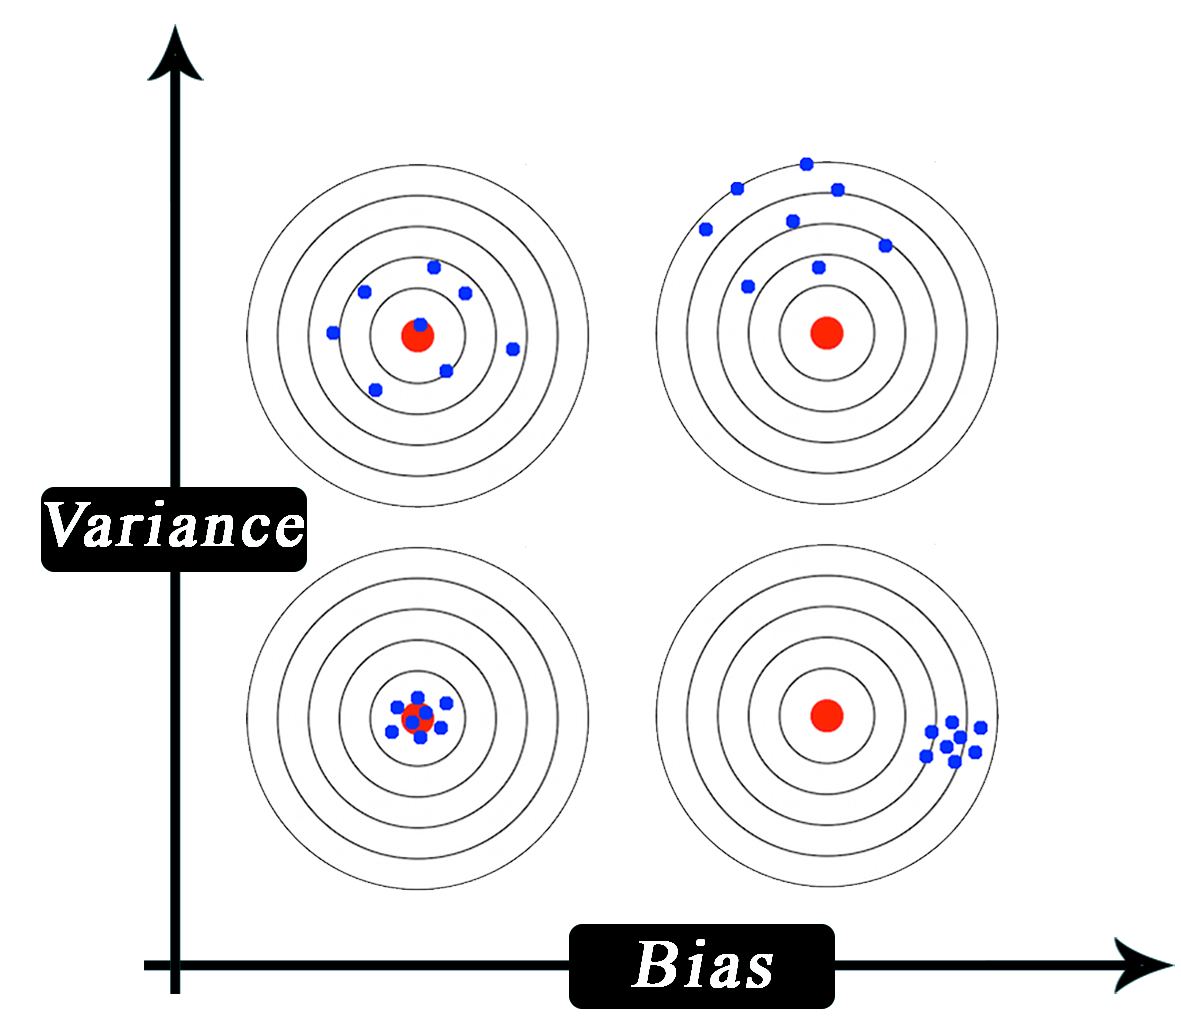
\includegraphics[width=7cm]{img/biasV.png}\hfill
            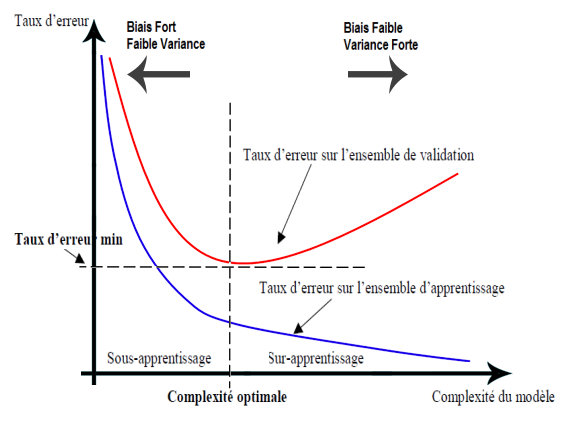
\includegraphics[width=9cm]{img/biasV3.png}
            \caption{Bias-Variance Tradeoff}\label{biasVar}
            \end{figure}
    \end{itemize}
\end{itemize}








\newpage
\markboth{}{}
\setcounter{mtc}{11}
\chapter[Préparation des données]{Préparation des données}
\label{dataprepation}
\chapterabstract
{
Dans ce chapitre nous allons expliciter les différentes étapes abordées dans la préparation des données utilisés dans ce travail, comme l’extraction des données à partir des prévisions du modèle de prévision numérique du temps (AROME, modèle opérationnel à la Direction de la Météorologie Nationale), les transformations des données et la construction de la base de données finale. Vers la fin de ce chapitre, nous allons expliquer l'approche adoptée pour la répartition et l’échantillonnage de ces données en deux fichiers (test et apprentissage) afin de garantir la représentativité des mois, des heures et des diverses classes de visibilités pour toutes les stations synoptiques.
}
\pagestyle{plain}

La préparation des données consiste à transformer les données brutes en des ressources d'information compréhensible et affinées. C'est une étape fondamentale de l'analyse des données en général et du Datamining en particulier. Cette activité comprend plusieurs tâches à savoir l'acquisition et le chargement des données, contrôle de la qualité des données, et la transformation des données lorsqu'il le faut. \\

Le jeu de données utilisées dans ce travail est déjà préparé dans une étude réalisée à la Direction de la Météorologie Marocaine par \citep{Ouagabi-Bari2018}. Dans ce qui suit, nous allons présenter brièvement les grandes phases de préparation des données, ainsi que la configuration de l'échantillonnage adoptée au cours de ce travail (Cf. Fig. \ref{rep_donnees}).\\

La base de données utilisée dans ce travail couvre les données horaires de 3 ans (2014, 2015 et 2016), résultat d’un prétraitement des sortie brutes du modèle de prévision numérique AROME et des données observées.\\

\begin{tcolorbox}
\footnotesize {
Le modèle non-hydrostatique AROME \citep{seity2011arome} est le modèle de prévision numérique du temps à maille fine exploité en opérationnel à la Direction de la Météorologie Nationale. Il a été conçu pour améliorer la prévision à courte échéance des phénomènes dangereux tels que les fortes pluies méditerranéennes, les orages violents, le brouillard ou les îlots de chaleur urbains en période de canicule. Il a été développé grâce à d’étroites collaborations, nationales et internationales, afin de tenir compte des dernières avancées en modélisation atmosphérique.
}
\end{tcolorbox}

Les fichiers de données brutes issues des prévisions d’AROME sont considérés comme les fichiers en entrée du package FullPos.

\begin{tcolorbox}
\footnotesize {
FullPos est un package de post-traitement puissant et sophistiqué. Il est destiné à être utilisé pour l'exploitation et la recherche. FullPos a deux parties principales : les interpolations verticales, puis les interpolations horizontales. Entre les deux, un traitement spectral est parfois possible pour les champs dynamiques.
}
\end{tcolorbox}

Ci-dessous les grandes étapes qui sont établis au cours de préparation et de traitement des sorties du modèle AROME:
\begin{enumerate}
    \item Application du FullPOS sur les fichiers bruts de prévision en format LFI par jour et par échéance ;
    \item Extraction des 29 paramètres météorologiques qui seront utilisés comme prédicteurs par date, heure, latitude et longitude de chaque point de grille du domaine d’étude ;
    \item Extraction des lignes correspondantes aux points de grille le plus proche de chaque station
synoptique du domaine d’étude ;
    \item Transformation des données générées au format adéquat à l’utilisation lors de la phase de
modélisation et génération de la direction et de la vitesse du vent à partir des composantes
zonale et méridionale du vent ;
\end{enumerate}

\section{Traitement des sorties brutes du modèle AROME}
\ding{109} L’extraction des sorties du modèle de prévision numérique du temps (PNT) a été réalisé par un script développé à base du FullPoss, avec une durée d’une semaine sur le super calculateur IBM de Maroc Météo. Ainsi, une conversion en format ASCII a été établi sur les données stocké dans les fichiers FullPoss de taille 128 mo/fichier. Ainsi, la taille globale a atteint 128 mo/fichier x 24 fichier/jour x 365 jours/an x 3 ans = 3363840 mo= 3.36To). \\

\ding{109} Transformation des données inclut le calcul de nouveaux champs ainsi la conversion des unités de mesure pour quelques variables comme il est présenté dans la table \ref{tabl_trans}.
\begin{table}[ht]
\begin{center}
\begin{tabular}{ |c|c|c| } 
\hline
\textbf{Variable} & \textbf{transformation} & \textbf{équation} \\
\hline
CLSTEMPERATURE & Kelvin -> \degree C & CLSTEMPERATURE-273.15\\
\hline
CLSHUMI.RELATIVE & Décimale -> \% & CLSHUMI.RELATIVEx100\\
\hline
MSLPRESSURE & Bar -> millibar & MSLPRESSURE/100\\
\hline
H00010TEMPERATUR & Kelvin -> \degree C & H00010TEMPERATUR-273.15\\
\hline
H00010HUMI\_RELAT & Décimale -> \% & H00010HUMI\_RELATx100\\
\hline
H00010TEMPE\_POTE & Kelvin -> \degree C & H00010TEMPE\_POTE-273.15\\
\hline
H00010THETA\_PRIM & Kelvin -> \degree C & H00010THETA\_PRIM-273.15\\
\hline
H00010PRESSURE & Bar -> millibar & H00010PRESSURE/100\\
\hline
SURFPRESSION & Bar -> millibar & SURFPRESSION/100\\
\hline
\end{tabular}
\caption{Les transformation sur les champs des sorties du modèle PNT}\label{tabl_trans}
\end{center}
\end{table}

\section{Traitement des données observées brutes}
Les données météorologiques utilisées dans cette étude sont extraites des Comptes Rendus Quotidiens
(CRQ) issus de chacune des stations synoptiques incluses dans la zone d’étude, et regroupée tous dans
un fichier texte. Ainsi, un prétraitement a été établi sur ces données afin de:
\begin{itemize}
    \item[\ding{230}] Supprimer les lignes avec données manquantes en visibilité.
    \item[\ding{230}] Supprimer des lignes avec des données aberrantes en visibilité (valeurs qui dépassent
30000m)
    \item[\ding{230}] Extraire des données issues des stations faisant partie du domaine (longitude entre -0.045 et
-10.295 ; latitude entre 28.64 et 37.84) et de la période d’étude.
\end{itemize}

\section{Préparer la base de données finale}
Après l'extraction et les transformations des donnée, la phase de la fusion des données dans un fichier final a été effectuée. Voici les étapes suivies pour fusionner ces données: 
\begin{enumerate}
    \item Extraire les données météorologiques observées correspondantes à la première station;
    \item Extraire les prévisions du modèle AROME correspondants au point de grille le plus proche à la
première station;
    \item Fusionner les deux ensembles de données qu’on vient d’extraire par jointure en passant la date
et l’heure comme clé de cette jointure, incluant tous les paramètres du modèle AROME, et
seulement la visibilité observée à partir des données météorologiques;
    \item Insérer le résultat de cette jointure dans un fichier de données final;
    \item Refaire le même processus pour les autres stations, et les rassembler toutes dans un fichier final.
\end{enumerate}
\section{Échantillonnage des données en sous-ensembles d'apprentissage et de test}
le fichier final, construit le jeu de données de notre étude, a été subdivisé en:\\

\begin{itemize}
    \item[\ding{230}] \textbf{Fichier d’apprentissage} : permet au modèle développé d’apprendre et de s’adapter par comparaison entre le résultat qu’il calcule en fonction des entrées fournies, et la réponse attendue en sortie. La taille de ce fichier dans ce travail constitue 70\% du fichier final;\\
    
    \item[\ding{230}] \textbf{Fichier de test} : contient des données indépendantes du fichier d’apprentissage et permet de tester la performance du modèle développé. La taille de ce fichier constitue 30\% du fichier final.\\
\end{itemize}

L'approche adoptée pour la répartition et l’échantillonnage de ces données en deux fichiers (test et apprentissage) garantit la représentativité des mois, des heures et des diverses classes de visibilités pour toutes les stations synoptiques (Cf. Fig. \ref{rep_donnees}). Ceci est fait dans le but d'éliminer certains facteurs qui peuvent biaiser la performance des modèles développés pour l'estimation de la visibilité horizontale à partir des sorties du modèle AROME :\\


\begin{itemize}
    \item[\ding{109}] \textbf{chaque Station}: pour assurer que toutes les stations utilisées ont été prises en compte lors de la phase d'apprentissage et de test.
    \item[\ding{109}] \textbf{chaque mois}: pour que le modèle développé soit entraîné sur toute les saisons de l'année.
    \item[\ding{109}] \textbf{chaque heure}: pour s'assurer que les modèles développés ont pris compte tous les moments de la journée.
    \item[\ding{109}] \textbf{chaque classe de visibilité}: pour que les modèles prennent en charge les 3 possibilité de la visibilité allant de la plus réduite jusqu'aux bonnes conditions \footnote{Classe C1 (visibilité<1km), C2 ( $1 km \le visibilité  < 5km$) et C3 (visibilité $\ge$ 5km)}.
\end{itemize}



\newpage
\begin{landscape}
\begin{figure}[!h]
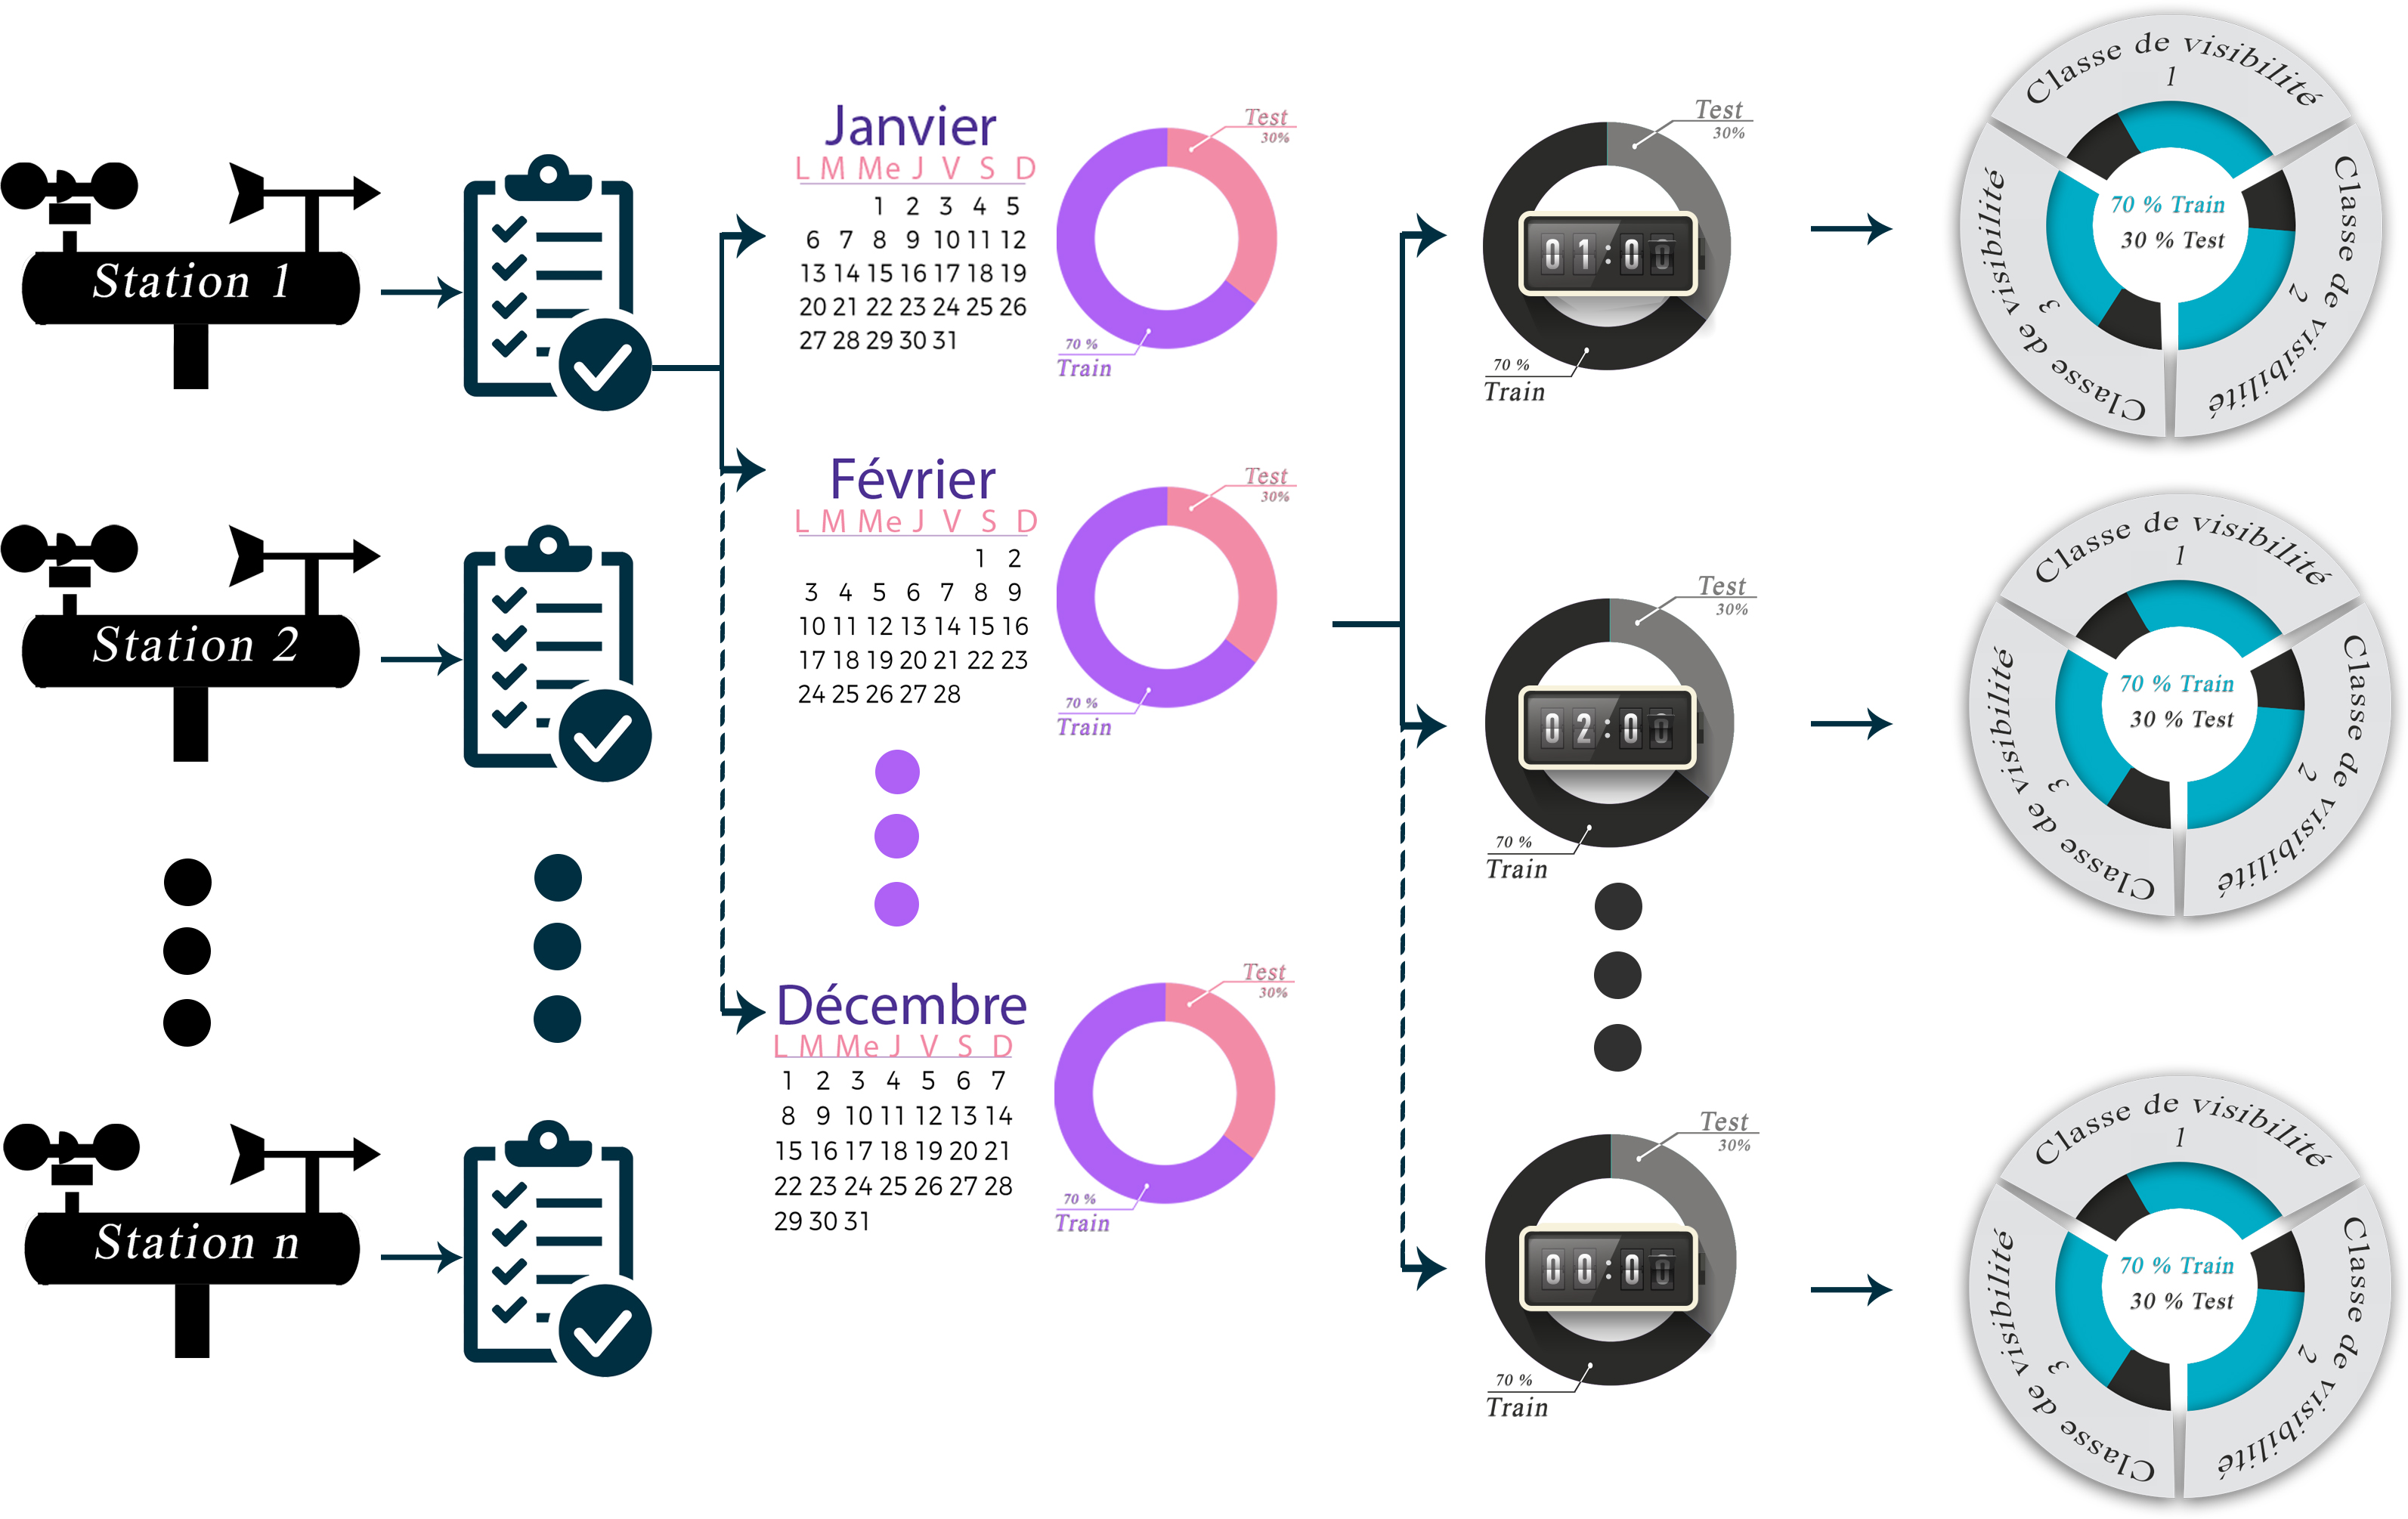
\includegraphics[width=23 cm, height= 14 cm]{img/data_prep.jpg}
\caption{La répartition des données}
\label{rep_donnees}
\end{figure}
\end{landscape}


\newpage
\markboth{}{}
\setcounter{mtc}{12}
\chapter[Modélisation]{Modélisation}
\label{Modelisation}

\chapterabstract
{
Au cours de ce chapitre, la phase de développement informatique effectué pendant cette étude, ainsi que les phases de conception et de développement des modèles de prédiction grâce au Datamining dans les différentes plateformes seront présentées. Notamment, nous expliquerons en détails les grandes étapes d'installation et de configuration des outils Datamining, ensuite nous allons développer un modèle pour chaque algorithme avec les paramètres choisis par défauts pour chaque plateforme, puis nous chercherons le meilleur modèle après optimisation des hyperparamètres de ces algorithmes.
}
\pagestyle{plain}

\section{Développement informatique}\label{conf_plat}
Avant d'entamer la phase de développement des modèles de prédiction sélectionnés pour ce travail (RF, GBM, XGB et Deep learning). L'installation et la configuration des différents plateformes open source utilisées dans cette étude (\textit{WEKA}, \textit{H2O}, \textit{Scikit-learn}, \textit{Tensorflow} et \textit{Keras}) m'a exigé une période assez importante. Bien évidemment, cette phase a consisté à comprendre et à se familiariser avec le mode de fonctionnement et d’implémentation de chaque plateforme, ainsi que les librairies Datamining y incluses. En effet, cette phase m'a permis d'approfondir mes connaissances dans le domaine du  Datamining.\\

Il est à noter que toutes ces plateformes, packages et bibliothèques sont installés et configurés sur un ordinateur portable HP avec 12 Gb en RAM \footnote { Random Access Memory} et un processeur Intel\textregistered core\texttrademark i7 – 2620M CPU @ 2.70 GHz (4CPUs) $\thicksim$ 2.7 GHz. Cet ordinateur a un système d'exploitation Windows 10 (version 1803) (Cf. Fig. \ref{pc_config}). Ainsi l'installation de ces outils est établie avec des versions stable à la date de mars 2019.\\

\begin{figure}[!htb]
        \center{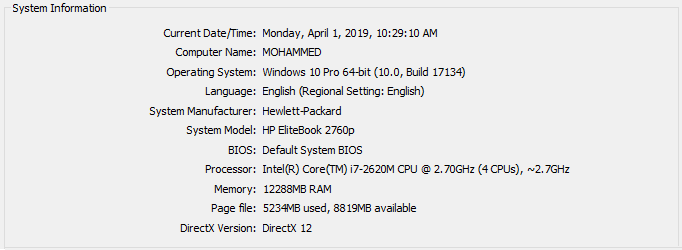
\includegraphics[width=\textwidth]{img/config.png}}
        \caption{\label{fig:my-label} Configuration de l'ordinateur utilisé pour ce travail}
        \label{pc_config}
\end{figure}


Dans la suite, les étapes de l'installation et la configuration de chaque outil Datamining sont explicitées:\\


Tout d'abord, nous avons installé la version stable 3.8 (13 février 2019) du logiciel \textit{WEKA} (Cf. Section \ref{defWeka}) qu'on a téléchargé depuis le site web officiel de l'application (www.cs.waikato.ac.nz). Ce qui a nécessité d'installer la version adaptée à Windows 10 ainsi la machine virtuelle Java VM 1.8. Une fois l'installation est terminée, nous avons augmenté l'espace mémoire allouée à Weka (heap size) de 256M par défaut à 4096M ‬pour qu'il prenne en charge les données de grande taille et d'éviter les problème de saturation de la mémoire au cours de l'exécution les phases d'apprentissage.\\

Pour la deuxième plateforme \textit{H2O} (Cf. Section \ref{defH2O}), l'algorithme \textit{XGBoost} n'a pas fonctionné pas sous H2O en Windows, donc on était obligé d’installer la plateforme H2O sous Linux.  Dans notre étude, l'installation a été effectuée sous une machine virtuelle de Linux. Cette tâche a été effectuée sous Linux Ubuntu 16.04 dans VMware Workstation avec la configuration suivante : 8GB en RAM, 2 processeurs et 30GB comme espace physique.
Une fois installé, nous avons téléchargé le fichier h2o-3.22.1.6.zip « dernière version stable à la date du 28/03/2019 » depuis le site web officiel de la plateforme (https://www.h2o.ai/).\\

Puisque \textit{H2O} se base principalement sur Java, nous avons installé openJDK 1.8. Avec la commande suivante nous pouvons lancer \textit{H2O} :
\begin{figure}[!htb]
        \center{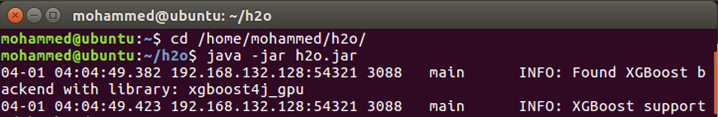
\includegraphics[width=\textwidth]{img/lanceh2o.png}}
\end{figure}

A l'issue de cette étape, nous avons le droit d’utiliser \textit{H2O} en mode web (FLOW) dans le système Windows « il suffit de taper l’adresse + port dans le navigateur (198.168.132.128 :54321 dans notre cas) ». Et pour pouvoir utiliser Python ou R, il suffit d’installer le même package \textit{h2o} (c’est-à-dire 3.22.1.6). Au cours de ce stage, nous avons opté pour le langage R. \\

\begin{wrapfigure}{r}{0.2\textwidth}
    
\includegraphics[width=0.2\textwidth]{img/condalogo.png}
\end{wrapfigure}
Pour les trois derniers outils ils ont basé principalement sur Python, alors nous avons travaillé avec Anaconda Navigateur\footnote{C'est une distribution libre et open source des langages de programmation Python et R appliqué au développement d'applications dédiées à la science des données et à l'apprentissage automatique, adaptés pour Windows, Linux et MacOS.} 3.7.1 avec une version de Python 3.7 pour \textit{Scikit-learn} et 3.6 pour \textit{Tensorflow} et \textit{Keras}.\\

Une phase préliminaire a consisté en l'installation des packages \textit{numpy} et \textit{scipy} qui sont des paquets requis pour installer \textit{Scikit-learn} ( C'est déjà expliqué dans la section \ref{defscikit}). Le moyen le plus simple d’installer \textit{Scikit-learn} consiste à utiliser \textbf{pip}\footnote{
Pip est un acronyme récursif pouvant signifier "Pip Installe des packages" ou "Pip Installe Python", c'est un outil de gestion des packages de distribution en Python} donc une fois l’installation d’Annoconda est terminé nous avons installé notre paquet \textit{Scikit-learn} en utilisant l’invite de commande annaconda comme ci-dessous:
\begin{tcolorbox}
\normalsize pip install -U scikit-learn
\end{tcolorbox}	
Ou en utilisant la command \textbf{conda} :
\begin{tcolorbox}
\normalsize conda install scikit-learn
\end{tcolorbox}	
Sous l’environnement par défaut de la distribution Anaconda. \\

Concernant \textit{Tensorflow} (Cf. Section \ref{defTensor}) et \textit{Keras} (Cf. Section \ref{defKeras}), nous étions obligé de créer un nouvel environnement Anaconda, puis l'activer pour installer les packages \textit{Tensorflow} et \textit{Keras} qui nécessite la version Python 3.6. Les étapes d'installation sont expliqués ci-dessous: \\

\begin{enumerate}
\item La création d'un environnement conda nommé « tensorflow » (vous pouvez changer le nom) en appelant la commande suivante :
\begin{tcolorbox}
\normalsize conda create -n tensorflow pip python=3.6
\end{tcolorbox}	
\item L'activation de l'environnement Conda en exécutant la commande suivante :\\
\begin{tcolorbox}
\normalsize activate tensorflow
\end{tcolorbox}	
\end{enumerate}
Une fois cette configuration est terminée, nous somme prêt à installer les bibliothèques Python utilisées pour \textit{Deep Learning}, notamment : \textit{TensorFlow} et \textit{Keras}.\\

Pour installer \textit{TensorFlow}, taper la commande suivante :
\begin{tcolorbox}
\normalsize pip install tensorflow
\end{tcolorbox}


Finalement pour installer la dernière API \textit{Keras}, on vérifie tout d'abord la présence de l’un de ses moteurs : \textit{TensorFlow}, \textit{Theano} ou \textit{CNTK}. 
il suffit de taper la commande suivante:\\
\begin{tcolorbox}
\normalsize pip install keras
\end{tcolorbox}




%%%%%%%%%%%%%%%%%%%%%%%%%%%%%%%%%%%%%%%%%%%%%%%%%%%%%%%%%%%%%%%%%%%%%%%%%%%%%%%%%%%%%%%%%%%%%%%%%%%%%%%%%%%%%%%%%%%%%%%%%%%%%%%%
\section{Développement des modèles de prédiction}
Au cours de notre étude, nous avons utilisé les méthodes du Datamining de famille d’estimateurs suivants: \textit{Random Forest} (RF), \textit{ Gradient Boosting Machine} (GBM) et \textit{eXtreme Gradient Boosting} (XGBoost), ainsi que \textit{Deep learning}. La théorie de ces algorithmes est explicitée succinctement dans la section \ref{algo_used}.\\

Pour mener à terme cette phase de modélisation, les étapes suivies pour développer chaque algorithme étaient comme suit :
\begin{enumerate}
    \item Importation des deux fichiers de données (donnée d'apprentissage et de test);
    \item Spécification des variables indépendantes (X\_train et X\_test)  et dépendant (y\_train et y\_test);
    \item Génération du modèle de prévision à partir des sorties du modèles de prévision numérique du temps AROME pour chaque algorithme par plateforme à la base des données d'apprentissage : dans un premier temps en utilisant les paramètres par défaut, ensuite en utilisant les hyperparamètres issus des méthodes d'optimisation décrites en section \ref{opt_algo};
    \item Évaluation de la performance du modèle développé en utilisant les données de test pour calculer les indices de diagnostic expliqués dans la section \ref{dig_algo_perf}.\\
\end{enumerate}

Il est à noter que pour le développement du modèle à la base de \textit{Deep learning} a nécessité la normalisation de données.\\

Dans ce qui suit, nous allons expliciter les fourchettes des hyperparamètres qu'on a utilisé au cours de ce stage pour leur optimisation afin d'obtenir le modèle par algorithme et par plateforme.\\
%%%%%%%%%%%%%%%%%%%%%%%%%%%%%%%%%%%%%%%%%%%%%%%%%%%%%%%%%%%%%%%%%%%%%%%%%%%%%%%%%%%%%%%%%%%%%%%%%%%%%%%%%%%%%%%%%%%%%%%%%%%%

\subsection*{Les hyperparamètres avec Random Search et Grid Search}\label{hyper_param}

Le réglage des hyperparamètres est une étape nécessaire lors la phase de modélisation en Machine learning. Elle permet de tester différentes configurations d'hyperparamètres pendant l'entraînement du modèle. Ces réglages peuvent fournir au développeur des valeurs optimisées pour les hyperparamètres, ce qui permet d'améliorer la précision des prédictions du modèle.\\

L'application d'entraînement gère trois catégories de données pendant l'entraînement du modèle à développer :

\begin{itemize}

\item[\ding{224}]    \textit{Les données d'entrée} (également appelées données d'entraînement) sont un ensemble d'enregistrements individuels (instances) contenant les caractéristiques importantes de la problématique de machine learning. Ces données sont utilisées pendant l'entraînement pour configurer le modèle afin qu'il puisse réaliser des prédictions précises à partir de nouvelles instances de données similaires. \\

\item[\ding{224}]   \textit{Les paramètres} du modèle sont les variables que la technique de machine learning sélectionnée utilise pour s'adapter aux données. Par exemple, un réseau de neurones profond (Deep Neural Network ou DNN) est composé de nœuds de traitement (neurones). Chacun d'entre eux effectue une opération spécifique sur les données lors de leur propagation à travers le réseau. Lorsque le DNN est entraîné, chaque nœud possède une valeur de pondération qui indique au modèle l'impact de ce nœud sur la prédiction finale. Ces pondérations sont un exemple de paramètres associés au modèle. \\

\item[\ding{224}]     \textit{Les hyperparamètres} sont les variables qui régissent le processus d'entraînement lui-même. Par exemple, une partie de la configuration d'un réseau de neurones profond consiste à décider combien de couches de nœuds cachées seront utilisées entre la couche d'entrée et la couche de sortie, ainsi que le nombre de nœuds que chaque couche doit utiliser. Ces variables ne sont pas directement liées aux données d'entraînement. Ce sont des variables de configuration. Notez que les paramètres changent au cours d'une tâche d'entraînement, alors que les hyperparamètres sont généralement constants pendant une tâche.\\
\end{itemize}

Dans ce qui suit, nous résumons dans des tableaux les fourchettes utilisées pour l'optimisation des hyperparamètres pour les plateformes \textit{Scikit-learn} et \textit{H2O} à la base deux méthodes : Grid-Search et Random-Search. \\

\begin{itemize}
    \item[\ding{233}]\textbf{Random Forest}\\%%%%%%%%%%%%%%%%%%%%%%%%%%%%%%%%%%%%%%%%%%%%%%%%%%%%%%%%%%%%%%%%%%%
        Les principaux hyperparamètres pour l'algorithme Random Forest sont récapitulés dans le tableau \ref{tab:HP-RF-OP}.\\
        
        \begin{table}[h!]
        \centering
        \begin{tabular}{|c|c|p{7cm}p{0.2cm}|}
        \hline
        plateforme & hyperparamètre &\multicolumn{2}{|c|}{Intervalle de variation}  \\ \hline
        \multirow{6}{*}{Scikit-learn} 
        & n\_estimators &  [60,80] avec un pas de 5 &\\
        & min\_samples\_split & [2,3,4] &\\ 
        & min\_samples\_leaf & [1,2,3,4] &\\
        & max\_features & ['auto','sqrt','log2', 'n/3'] avec n nombre d'observations &\\
        & max\_depth & [1, 6, 11, 17] &\\
        & bootstrap & [True, False] &\\
         \hline
        \multirow{6}{*}{H2O} 
        & ntrees &  [50,100] avec un pas de 10 &\\
        & max\_depth & [10,17] avec un pas de 1  &\\
        & min\_rows & [1,5] avec un pas de 1 &\\
        & mtries & [-1, 3] avec un pas de 1 &\\
         \hline
        \end{tabular}
        \caption{Liste des intervalles des hyperparamètres pour RF\\}
        \label{tab:HP-RF-OP}
        \end{table}
        
        \item[\ding{233}]\textbf{Gradient Boosting Machine}\\%%%%%%%%%%%%%%%%%%%%%%%%%%%%%%%%%%%%%%%%%%%%
Les principaux hyperparamètres pour l'algorithme Random Forest sont récapitulés dans le tableau \ref{tab:HP-GBM-OP}.
        \begin{table}[h!]
        \centering
        \begin{tabular}{|c|c|p{7cm}p{0.2cm}|}
        \hline
       plateforme & hyperparamètre &\multicolumn{2}{|c|}{Intervalle de variation} \\ \hline
        \multirow{6}{*}{Scikit-learn} 
        & n\_estimators & [100, 200] avec un pas de 25 &\\
        & min\_samples\_split & [2,3,4]  &\\ 
        & min\_samples\_leaf & [1,2,3,4] &\\
        & max\_features & ['auto','sqrt','log2', 'n/3'] avec n nombre d'observations &\\
        & max\_depth & [1,15] avec un pas de 5 &\\
        & learning\_rate  & [0.01, 0.025, 0.05, 0.075, 0.1, 0.15, 0.2] &\\
         \hline
        \multirow{4}{*}{H2O} 
        & ntrees & [200,400] avec un pas de 50 &\\
        & max\_depth & [5, 17] avec un pas de 2 &\\
        & min\_rows & [2,5,10] &\\ 
        & sample\_rate & [0.5, 0.8, 0.95, 1.0] &\\
         \hline
        \end{tabular}
        \caption{Liste des intervalles des hyperparamètres pour GBM}
        \label{tab:HP-GBM-OP}
        \end{table}
 
        \item[\ding{233}]\textbf{eXtreme Gradient Boosting}\\%%%%%%%%%%%%%%%%%%%%%%%%%%%%%%%%%%%%%%%%%%
Les principaux hyperparamètres pour l'algorithme \textit{Random Forest} sont récapitulés dans le tableau \ref{tab:HP-XGB-OP}.
        \begin{table}[h!]
        \centering
        \begin{tabular}{|c|c|p{5.8cm}p{0cm}|}
        \hline
       plateforme & hyperparamètre &\multicolumn{2}{|c|}{Intervalle de variation} \\ \hline
       \multirow{5}{*}{Scikit-learn} 
        & n\_estimators & [100,200] avec un pas de 10  &\\
        & gamma & [0,5] avec un pas de 1 &\\ 
        & colsample\_bytree & [0.8, 1.0] avec un pas de 0.05 &\\
        & learning\_rate & [0.01, 0.025, 0.05, 0.075, 0.1, 0.15, 0.2] &\\
        & max\_depth & [3,15] avec un pas de 3 &\\
         \hline
        \multirow{6}{*}{H2O} 
        & ntrees &   [100,400] avec un pas de 100 &\\
        & max\_depth & [5, 10, 17] &\\
        & min\_rows &  [2, 5, 11] &\\ 
        & sample\_rate & [0.5, 0.8, 0.95, 1.0] &\\
        & col\_sample\_rate & [0.5, 0.8, 0.95, 1.0] &\\
        & col\_sample\_rate\_per\_tree & [0.8, 0.99, 1.0] &\\
         \hline
       \end{tabular}
               \caption{Liste des intervalles des hyperparamètres pour XGBoost}
               \label{tab:HP-XGB-OP}
        \end{table}
\end{itemize}


\newpage
\setcounter{mtc}{13}
\chapter[Évaluation de la performance du modèle développé]{Évaluation}
\label{evaluation}

\chapterabstract
{
Dans ce chapitre nous évaluerons les performances des modèles élaborés grâce au Datamining. Ainsi, l'analyse des résultats sera effectuée dans le sens d'étudier la sensibilité d'un modèle à la plateforme et l'algorithme utilisé pour le développer. Nous présenterons du premier temps les résultats de comparaison entre les déférents  algorithmes utilisés au sein de ce travail puis la performance de chaque algorithme dans les déférents plateformes, et nous terminerons par une analyse croisées par plateforme et par algorithme. 
}
\pagestyle{plain}

%%%%%%%%%%%%%%%%%%%%%%%%%%%%%%%%%%%%%%%%%%%%%%%%%%%%%%%%%%%%%%%%%%%%%%%
\section{Comparaison des plateformes open source utilisées}\label{comp_plat}
%%%%%%%%%%%%%%%%%%%%%%%%%%%%%%%%%%%%%%%%%%%%%%%%%%%%%%%%%%%%%%%%%%%%%%%
Jour après jour, l'importance du \textit{Datamining} augmente et le nombre d'outils disponibles continue à croître. Par conséquence, le choix de l'outil le plus approprié devient de plus en plus difficile. Pour cette raison et d'autres, la comparaison des outils d'exploration des données (KDD = Konwledge Discovery from Database) devient importante.\\

La comparaison entre plateformes open sources n’est pas évidente car elle
fait  appel  à  plusieurs  critères  (structures  de  données,  les  algorithmes
implémentés, capacités de visualisation, langages de programmation, options
d’importation et d’exportation, etc.). Pour ce faire, on s’est focalisé sur les
critères  suivants  et  qui  ont  été  adoptés  par  \cite{chen2007survey}  :  les
caractéristiques générales, la gestion des données, leur fonctionnalité et le mode
d’utilisation. Le tableau \ref{comp_tabl_cg} illustre une comparaison des caractéristiques générales des outils Datamining utilisée.\\

\begin{table}[ht]
\begin{center}
\begin{threeparttable}[t]
\begin{tabular}{ |l|c|c|c|c| }
\hline

\hline
    \textbf{Produit} 
    & \textbf{Architecture} 
    & \textbf{SE} 
    & \textbf{Language} 
    & \textbf{CPU / GPU} \\ 
\hline

\hline
\multirow{3}{*}{WEKA}
 & {Client/Server} & {Linux} & {Java} & {CPU} \\
 & {Standalone} & {Mac OS X} & {} & {} \\
 & {} &{Windows} & {} & {}\\
 \hline
 \multirow{3}{*}{H2O}
 & {Client/Server} & {Linux Ubuntu} & {Java, Scala,} & {CPU} \\
 & {Standalone} & {Mac OS X} & {Python, R,} & {GPU} \\
 & {Cloud service} &{Windows} & {Json} & {}\\
 \hline
 \multirow{3}{*}{Scikit-learn}
 & {} & {Linux} & {} & {} \\
 & {Client/Server} & {Mac OS X} & {Python} & {CPU} \\
 & {} &{Windows} & {} & {}\\
 \hline
 \multirow{3}{*}{Tensorflow}
 & {Client/Server} & {Linux} & {Python} & {CPU} \\
 & {Cloud service} & {Windows} & {C++} & {GPU} \\
 & {} &{Mac OS X} & {Java} & {TPU\tnote{1}}\\
 \hline
 \multirow{3}{*}{Keras}
 & {Client/Server} & {Linux} & {Python} & {CPU} \\
 & {Cloud service} & {Windows} & {R, Scala} & {GPU} \\
 & {} &{Mac OS X} & {Java} & {}\\
 \hline

 \hline
\end{tabular}
\footnotesize{
            \begin{tablenotes}
                  \item[1]  Tensor Processing Unit, un type de processeur dédié au calcul d'apprentissage des réseaux de neurones
            \end{tablenotes}
        }
\end{threeparttable}
\caption{Les caractéristiques générale des plateformes}\label{comp_tabl_cg}
\end{center}
\end{table}

L’architecture de \textit{WEKA} peut être autonome (standalone) ou clien/serveur, et elle peut fonctionner sous Windows, MAC et Linux, et s'exécute en CPU.
\textit{WEKA} est développé en Java et les algorithmes peuvent soit être appliqué directement à un jeu de données ou appelé par un code Java, ou par l'API Java.\\

\textit{H2O} utilise une interface utilisateur open source basée sur le Web (FLOW). Elle peut fonctionner sur les systèmes d’exploitation Windows, OS X et Ubuntu, et s'exécute en CPU/GPU et permet la programmation en R, Python, Scala, Java et JSON. Ainsi qu'il y a une possibilité de lancer \textit{H2O}
sur un cluster Hadoop. \textit{H2O} est pris en charge sur un certain nombre de cloud environnements.\\

\textit{Scikit-learn} peut fonctionner sur les différents systèmes d'exploitation Windows, Linux et Mac OS; avec quelques prérequis: (Python ($\geq$ 2.7 ou $\geq$ 3.4), NumPy ($\geq$ 1.8.2), SciPy ($\geq$ 0.13.3)). Il ne supporte pas GPU mais il s'exécute facilement dans CPU, et permet de programmer en langage Python.\\

\textit{Tensorflow} peut fonctionner sur Windows, Linux et Mac OS, et permet la programmation en plusieurs langages mais les plus conviviaux et utilisés sont Python et C++. Ainsi, \textit{Tensorflow} s'exécute sous CPU comme sous GPU.\\

\textit{Keras} a une architecture client / serveur aussi qu'elle peut être fourni comme cloud service, Il est capable de fonctionner sur \textit{TensorFlow}. Fonctionne de manière transparente sur CPU et / ou GPU, permet de programmer en Python, R, Scala et Java (API Deeplearning4J).\\


Le deuxième critère de comparaison en plateformes est la façon de gestion des données. Le tableau \ref{comp_tabl_gd} présente les différentes sources et formats de données qu'un outil Datamining peut traiter, ainsi que la capacité de ce moyen à traiter les grandes masses de données (Big data).\\

\begin{table}[ht]
\begin{center}
\caption{La façon de gestion des données}\label{comp_tabl_gd}
\begin{tabular}{ |c|p{1cm}|p{0.8cm}|p{0.8cm}|p{0.8cm}|p{0.8cm}|p{0.8cm}|p{1.2cm}|p{1cm}|p{1cm}| } 
\hline
&\multicolumn{5}{|c|}{Source de données}
&\multicolumn{3}{|c|}{Format de données}
&{}\\
\hline
\textbf{Outil} & \textbf{J/O} & \textbf{S} & \textbf{E} & \textbf{OR} & \textbf{P} & \textbf{CSV} & \textbf{ARFF} & \textbf{URL} & \textbf{Size}\\
\hline
WIKA & \ding{51} & \ding{51} & \ding{53} & \ding{51} & \ding{51} & \ding{51} & \ding{51} & \ding{51} & \ding{51}$^*$\\
\hline
H2O & \ding{51} & \ding{53} & \ding{51} & \ding{53} & \ding{51} & \ding{51} & \ding{51} & \ding{51} & \ding{51}\\
\hline
Scikit-learn & \ding{51} & \ding{51} & \ding{51} & \ding{51} & \ding{51} & \ding{51} & \ding{51} & \ding{51} & \ding{51}\\
\hline
Tensorflow & \ding{51} & \ding{51} & \ding{51} & \ding{51} & \ding{51} & \ding{51} & \ding{51} & \ding{51} & \ding{51}\\
\hline
Keras & \ding{51} & \ding{51} & \ding{51} & \ding{51} & \ding{51} & \ding{51} & \ding{51} & \ding{51} & \ding{51}\\
\hline
\end{tabular}
J-JDBC O-ODBC S-MS SQL SERVER E-MS EXCEL OR-Oracle P-PostgreSQL\\
\ding{51} Support, \ding{53} Ne supporte pas, \ding{51}$^*$ Support avec limitation
\end{center}
\end{table}



Pour les fonctionnalités, chaque outil évolue d'une version à une autre afin de répondre à de nouvelles fonctionnalités et d'améliorer la liste de leurs capacités, ce qui rend encore plus le choix entre les plateformes plus difficile. Pour pouvoir résoudre différents problèmes d’exploration de données, la fonctionnalité d’une plateforme d’exploration de données open source est une propriété importante. Le tableau \ref{comp_tabl_f} présente le résumé des fonctionnalités des 5 plateformes. Les fonctions peuvent être divisées en huit groupes:
prétraitement des données, classification et prévision, regroupement (\textit{clustering}), règles d'association, évaluation et visualisation. Les outils d’exploration de données de base proposés incluent  les arbres de décision, les réseaux de neurones, les regroupements par les nuées (K-means) et les règles d’association, les techniques  de machines à vecteurs de support (SVM), les forêts aléatoires et d'autres. Il est à noter que les systèmes actuels d’exploration de données open source incluent déjà les fonctions d’exploration de données les plus couramment utilisées. La différence réside principalement dans les capacités de visualisation.\\

\begin{table}[ht]
\begin{center}
\caption{Les fonctionnalités}\label{comp_tabl_f}
\begin{tabular}{ |c|p{1cm}|p{1cm}|p{1cm}|p{1cm}|p{1cm}|p{1cm}|p{1cm}|p{1cm}|p{1cm}| } 
\hline
\textbf{Outil} & \textbf{DP} & \textbf{P} & \textbf{R} & \textbf{CS} & \textbf{C} & \textbf{L} & \textbf{V} & \textbf{E}\\
\hline
WIKA & \ding{51} & \ding{51}  & \ding{51} & \ding{51} & \ding{51} & \ding{51} & \ding{51} & \ding{51}\\
\hline
H2O & \ding{51} & \ding{51} & \ding{51} & \ding{51} & \ding{51} & \ding{51} & \ding{51} & \ding{51}\\
\hline
Scikit-learn & \ding{51} & \ding{51} & \ding{51} & \ding{51} & \ding{51} & \ding{51} & \ding{51} & \ding{51}\\
\hline
Tensorflow & \ding{51} & \ding{51} & \ding{51} & \ding{51} & \ding{51} & \ding{51} & \ding{51} & \ding{51}\\
\hline
Keras & \ding{51} & \ding{51} & \ding{51} & \ding{51} & \ding{51} & \ding{51} & \ding{51} & \ding{51}\\
\hline
\end{tabular}
DP-Pré-traitement P-Prédiction R-Régression CS-Classification C-Clustering L-régles d'association V-La Visualisation E-L'analyse exploratoire des données \\
\ding{51} Support, \ding{53} Ne supporte pas,
\end{center}
\end{table}

Pour le mode d'utilisation (Cf. Tab. \ref{comp_tabl_mu}), l'aspect convivialité décrit la facilité avec laquelle un système d'exploration de données open source peut être utilisé pour résoudre des problèmes réels dans différents environnements de données et de systèmes. Ainsi, les cinq plateformes sont utilisable soit par l'invite de commande ou par GUI, sauf \textit{Scikit-learn}, \textit{Tensorflow} et \textit{Keras} qui sont utilisable par CLI ou par un éditeur de code. \\

\begin{table}[ht]
\begin{center}
\caption{Mode d'utilisation}\label{comp_tabl_mu}
\begin{tabular}{ |c|p{1cm}|p{1cm}|p{2cm}|p{2cm}|p{1cm}|p{1cm}|p{1cm}|p{1cm}| } 
\hline
\textbf{Outil} & \textbf{GUI} & \textbf{CLI} & \textbf{Business application} & \textbf{Recherche} \\
\hline
WIKA & \ding{51} & \ding{51} & \ding{51} & \ding{51}\\
\hline
H2O & \ding{51} & \ding{51} & \ding{51} & \ding{51}\\
\hline
Scikit-learn & \ding{53} & \ding{51} & \ding{51} & \ding{51}\\
\hline
Tensorflow & \ding{53} & \ding{51} & \ding{51} & \ding{51}\\
\hline
Keras & \ding{53} & \ding{51} & \ding{51} & \ding{51}\\
\hline
\end{tabular}\\
GUI-Graphical user interface CLI-Command line\\
\ding{51} Support, \ding{53} Ne supporte pas
\end{center}
\end{table}

\cite{chen2007survey} ont adopté un système de notation subjective pour la classification des plateformes open source qu'il a exploré dans son article de recherche. Ainsi, il a calculé un score pour chaque plateforme en utilisant un poids subjectif affecté à chaque caractéristique en se basant sur l'expérience des auteurs avec les plateformes étudiées. Dans notre travail, nous avons opté pour une comparaison pseudo-objective en donnant une note de 1 ou 0 dans le cas où la caractéristique est offerte ou pas par la plateforme. Pour le cas des caractéristiques générales, on a opté pour une notation de 1 (moins souple qui n'offre pas beaucoup de choix) à 3 (plus souple qui offre plus de choix). Par conséquent, le système de notation a débouché sur les résultats récapitulés dans la table   \ref{tab:score-comp}.\\

\begin{table}[!h]
    \centering
    \begin{tabular}{|c|p{1.5cm}|p{1.5cm}|p{1.5cm}|p{1.5cm}|p{2.5cm}|}
       \hline
       \textbf{plateforme}  & \textbf{CG} & \textbf{GD} & \textbf{FN} & \textbf{MU} &\textbf{score final}\\ \hline
       WEKA  &  7 & 7.5 & 8 & 4 & 26.5\\
       H2O   &  11 & 7 & 8 & 4 & 30\\
       Scikit Learn &  6 & 9 & 8 & 3 & 26\\
       TensorFlow & 10 & 9 & 8 & 3 & 30\\
       Keras &  9 & 9 & 8 & 3 & 29\\ \hline
    \end{tabular}
    \footnotesize{\\ \ding{223} CG: Caractéristiques générales, \ding{223} GD: gestion de données \ding{223} FN: fonctionnalités, \\ \ding{223} MU: mode d'utilisation.}
    \caption{Score de comparaison des plateformes selon les critères : caractéristiques générales, gestion de données, fonctionnalités, et mode d'utilisation}
    \label{tab:score-comp}
\end{table}

Sur la base de l'analyse précédente, on constate que les plateformes \textit{H2O} et \textit{TensorFlow} prédominent globalement les autres plateformes. Ainsi, nous pouvons résumer principaux avantages des systèmes d'exploration de données open source comme suit:\\

\begin{itemize}
    \item[\ding{224}] Le support de plusieurs systèmes d'exploitation : GNU / Linux, Mac et MS / Windows sont supportés par presque toutes les plateformes étudiées.
    \item[\ding{224}] Nombre important d'algorithmes implémentés dans la plateforme : Chaque système a intégré de nombreux algorithmes de prétraitement et de modélisation des données. 
    \item[\ding{224}] Bon mode d'utilisation.\\
\end{itemize}

D'autre part, certaines plateformes open source présentent certaines limitations :\\

\begin{itemize}
    \item[\ding{224}] Manque de prise en charge de certaines sources et format de données
    \item[\ding{224}] Difficulté avec la prise en charge du Big Data (grand volume de données) 
    \item[\ding{224}] Mauvaise  documentation en termes de manuel d'utilisateur.\\
\end{itemize}


%%%%%%%%%%%%%%%%%%%%%%%%%%%%%%%%%%%%%%%%%%%%%%%%%%%%%%%%%%%%%%%%%%%%%%%
\section{Sensibilité à la plateforme}
%%%%%%%%%%%%%%%%%%%%%%%%%%%%%%%%%%%%%%%%%%%%%%%%%%%%%%%%%%%%%%%%%%%%%%%
Dans cette section, nous allons comparer la performance des modèles développés à la base des algorithmes Datamining disponibles ou qu'on a pu exécuter pour chaque plateforme open source. Ceci mettra en exergue la sensibilité de cette performance à la plateforme. Rappelons que cette comparaison est effectuée dans un cas de régression relatif à l'estimation de la visibilité horizontale à partir des prévisions des paramètres météorologiques issues du modèle de prévision numérique du temps opérationnel à la Direction de la Météorologie Nationale (AROME).\\

\subsection*{Scikit-learn}
Pour cette plateforme, nous avons utilisé les quatre algorithmes suivants : \textit{Random Forest}, \textit{Gradient Boosting}, \textit{eXtreme Gradient Boosting} et \textit{Deep Learning}. Dans un premier temps, nous avons évalué la performance des modèles développés, pour la configuration par défaut (Cf. Section \ref{config_pl_algo}), à la base des outils de diagnostics décrits en section \ref{dig_algo_perf} : le biais, l'erreur quadratique moyenne (RMSE) et l'erreur absolue moyenne (MAE) ainsi que le coefficient de corrélation (CC).\\ 

Le tableau \ref{sc_default} récapitule les statistiques d'évaluation et 
montre que le meilleur modèle obtenu utilise \textit{Random Forest} comme algorithme de base avec une erreur quadratique moyenne de l'ordre de 2022 m et une erreur absolue moyenne de 1259 m associée à une coefficient de corrélation dépassant 0.8. Il est à noter que les résultats mettent en évidence le fait que tous les modèles développés à la base des quatre algorithmes sous-estiment la visibilité horizontale (Biais négatif de l'ordre de -163 m pour \textit{Random Forest}). Les autres algorithmes affichent des performances similaires en ordre de grandeur avec de forte corrélation. Ainsi, le \textit{Deep learning} affiche la plus mauvaise performance avec une erreur absolue moyenne MAE=1810 m et une erreur quadratique moyenne RMSE=2543 m. \\ 

\begin{table}[!ht]
    \centering
    \begin{tabular}{ |c|p{2cm}|p{2cm}|p{2cm}|p{2cm}|  }
     \hline
     & \multicolumn{4}{|c|}{Évaluation des modèles sous Scikit-learn} \\
     \hline
     & CC & Biais & MAE & RMSE\\
     \hline
     RF & 0.88 & -163 &  1259 & 2022\\
     \hline
     GBM &  0.83 & -196 & 1652 & 2364 \\
     \hline
     XGB & 0.83 & -196 & 1656 & 2365\\
     \hline
     DL & 0.80 & -193 & 1810 & 2543 \\
     \hline
    \end{tabular}
    \caption{Résultat d'évaluation sous Scikit-learn avec les paramètres par défaut}
    \label{sc_default}
\end{table}
\\

Dans l'étape suivante, nous avons réglé les hyperparamètres en utilisant les deux techniques Grid Search et Random Search (Cf. Section \ref{hyper_param}) pour les algorithmes à base de méthode ensembliste (\textit{Random Forest}, \textit{Gradient Boosting} et \textit{extreme gradient boosting}). Ceci nous a permis d'obtenir le meilleur modèle pour chaque algorithme pour les hyperparamètres optimums. Les statistiques d'évaluation des modèles développés sont récapitulés dans le tableau \ref{sc_ev_Tuning}:\\

\begin{table}[!ht]
    \centering
    \begin{tabular}{ |c|c|p{2cm}|p{2cm}|p{2cm}|p{2cm}|  }
     \hline
     \multicolumn{2}{|c|}{} &\multicolumn{4}{|c|}{Évaluation des modèles sous Scikit-learn} \\
     \hline
     \multicolumn{2}{|c|}{} & CC & Biais & MAE & RMSE\\
     \hline
    \multirow{2}{*}{RF} &
     Random Search & 0.88 & -152 &  1268 & 1969\\
     & Grid Search & 0.89 & -157 & 1221 & 1942\\
     \hline
     \multirow{2}{*}{GBM} &
     Random Search & 0.88 & -154 & 1336 & 2030\\
     & Grid Search & 0.88 & -151 & 1305 & 2008\\
     \hline
     \multirow{2}{*}{XGB} &
     Random Search & 0.86 & -166 & 1427 & 2140\\
     & Grid Search & 0.88 & -149 & 1272 & 1972\\
     \hline
    \end{tabular}
    \caption{Résultat d'évaluation sous Scikit-learn en utilisant les deux méthodes d'optimisation}
    \label{sc_ev_Tuning}
\end{table}

La table \ref{sc_ev_Tuning} montre que la performance de tous les algorithmes s'améliore en comparaison avec les résultats basés sur la configuration par défaut. Ainsi, l'erreur quadratique moyenne passe de 2365 m à 1972 m pour \textit{extreme gradient boosting}, et de 2364 m à 2021 m pour \textit{gradient boosting}. La meilleure performance reste toujours associée à \textit{Random Forest} avec une erreur RMSE de 1942 m contre 2022 m pour la configuration par défaut. De plus, l'erreur MAE s'est nettement améliorée à son tour en passant de 1259 m à 1221 m associée à un biais toujours négatif de -157 m avec une forte corrélation dépassant 0.8.\\

Il est à noter que les meilleurs modèles sont obtenus en utilisant les hyperparamètres optimums issus de Grid Search et ceci est justifié par le fait qu'on a utilisé la même fourchette des hyperparamètres pour les deux techniques. Ainsi, il est évident que les scénarios de Random Search soit inclus dans ceux adoptés par Grid Search.\\

\ding{230} Ainsi, l'algorithme \textit{Random Forest} est le meilleur estimateur pour la plateforme \textit{Scikit-learn} dans notre cas d'étude, avec une erreur quadratique moyenne RMSE de 1942 m associé à un coefficient de corrélation de 0.89 et une erreur absolue moyenne MAE de 1221 m.

\subsection*{H2O}
De même pour la plateforme \textit{H2O}, nous avons utilisé les quatre algorithmes suivants : \textit{Random Forest}, \textit{Gradient Boosting}, \textit{eXtreme Gradient Boosting} et \textit{Deep Learning}. Dans un premier temps, nous avons évalué la performance des modèles développés, pour la configuration par défaut décrite en section \ref{config_pl_algo}, à la base des outils de diagnostics décrits en section \ref{dig_algo_perf} : le biais, l'erreur quadratqiue moyenne (RMSE) et l'erreur absolue moyenne (MAE) ainsi que le coefficient de corrélation (CC).\\ 

Le tableau \ref{h2O_default} récapitule les résultats d'évaluation et montre que le meilleur modèle obtenu est basé sur l'algorithme \textit{Random Forest} avec une erreur quadratique moyenne de l'ordre de 1953 m et une erreur absolue moyenne de 1246 m associée à une coefficient de corrélation dépassant 0.89. Il est à noter que les résultats mettent en évidence le fait que tous les modèles développés à la base des quatre algorithmes sous-estiment la visibilité horizontale (Biais négatif de l'ordre de -156 m pour \textit{Random Forest}) sauf \textit{extreme gradient boosting} qui enregistre un biais presque parfait (proche de zéro). A l'exception de \textit{Random Forest}, les autres algorithmes affichent des performances similaires en ordre de grandeur avec de forte corrélation. \\ 
  
\begin{table}[!ht]
    \centering
    \begin{tabular}{ |c|p{2cm}|p{2cm}|p{2cm}|p{2cm}|  }
     \hline
     & \multicolumn{4}{|c|}{Évaluation des modèles sous H2O} \\
     \hline
     & CC & Biais & MAE & RMSE\\
     \hline
     RF & 0.89 & -156 & 1246 & 1953\\
     \hline
     GBM &  0.84 & -188 & 1550 & 2282 \\
     \hline
     XGB & 0.85 & 1 & 1547 & 2358\\
     \hline
     DL &  0.85 & -191 & 1544 & 2265\\
    \hline
    \end{tabular}
    \caption{Résultat d'évaluation sous H2O avec les paramètres par défaut}
    \label{h2O_default}
\end{table}

Dans l'étape suivante, nous avons réglé les hyperparamètres en utilisant les deux techniques Grid Search et Random Search (Cf. Section \ref{hyper_param}) pour les algorithmes à base de méthode ensembliste (\textit{Random Forest}, \textit{Gradient Boosting} et \textit{extreme gradient boosting}). Ceci nous a permis d'obtenir le meilleur modèle pour chaque algorithme pour les hyperparamètres optimums. Les statistiques d'évaluation des modèles développés sont récapitulés dans le tableau \ref{h2o_ev_Tuning}:\\

\begin{table}[!ht]
    \centering
    \begin{tabular}{ |c|c|p{2cm}|p{2cm}|p{2cm}|p{2cm}|  }
     \hline
     \multicolumn{2}{|c|}{} &\multicolumn{4}{|c|}{Évaluation des modèles sous H2O} \\
     \hline
     \multicolumn{2}{|c|}{} & CC & Biais & MAE & RMSE\\
     \hline
    \multirow{2}{*}{RF} &
     Random Search & 0.88 & -156 & 1299 & 2010\\
     & Grid Search & 0.88 & -157 & 1284 & 1982\\
     \hline
     \multirow{2}{*}{GBM} &
     Random Search  & 0.89 & -150 & 1189 & 1936\\
     & Grid Search & 0.89 & -145 & 1199 & 1933\\
     \hline
     \multirow{2}{*}{XGB} &
     Random Search  & 0.87 & 2 & 1357  & 2141 \\
     & Grid Search  & 0.87 & 6 & 1323  & 2164 \\
     \hline
    \end{tabular}
    \caption{Résultat d'évaluation sous H2O en utilisant les deux méthodes d'optimisation}
    \label{h2o_ev_Tuning}
\end{table}

La table \ref{h2o_ev_Tuning} montre que la performance de tous les algorithmes s'améliore en comparaison avec les résultats basés sur la configuration par défaut sauf pour \textit{Random Forest} qui enregistre une performance similaire. Ceci est dû au fait que les valeurs par défaut des hyperparamètres n'étaient pas incluses dans la fourchette adoptée pour le réglage des hyperparamètres. D'autre part, l'erreur quadratique moyenne passe de 2358 m à 2141 m pour \textit{extreme gradient boosting}, et de 2282 m à 1933 m pour \textit{gradient boosting machine} qui est associé à la meilleure performance. De plus, l'erreur MAE s'est nettement améliorée à son tour en passant de 1550 m à 1189 m associée à un biais toujours négatif de -150 m avec une forte corrélation dépassant 0.8. On constate aussi que l'algorithme \textit{XGBoost} enregistre un biais positive presque parfait au voisinage de zéro.\\

\ding{230} L'algorithme ensembliste adaptatif \textit{Gradient Boosting Machine}  est le meilleure estimateur de la visibilité pour la plateforme \textit{H2O} avec une erreur quadratique moyenne RMSE de 1933 m associé à un coefficient de corrélation de 0.89 et une erreur absolue moyenne MAE de 1199 m.  

\subsection*{WEKA}
Concernant la plateforme \textit{WEKA}, elle ne prend pas en compte les algorithmes \textit{Gradient Boosting Machine} et \textit{eXtreme Gradient Boosting}. Ainsi, les deux algorithmes suivants ont été utilisé : \textit{Random Forest} et \textit{Deep Learning}. Par conséquence, nous nous sommes limités aux paramètres par défaut pour évaluer la performance des modèles développés, à la base des outils de diagnostics décrits en section \ref{dig_algo_perf} :  l'erreur quadratqiue moyenne (RMSE) et l'erreur absolue moyenne (MAE) ainsi que le coefficient de corrélation (CC).\\ 

Le tableau \ref{weka_default} récapitule les résultats d'évaluation et montre que le meilleur modèle obtenu utilise \textit{Random Forest} comme algorithme de base avec une erreur quadratique moyenne de l'ordre de 1945 m et une erreur absolue moyenne de 1232 m associée à une coefficient de corrélation dépassant 0.89. Par contre, le \textit{Deep learning} affiche la plus mauvaise performance avec une erreur RMSE de 2645 m et une erreur MAE de 1923 m. 

\begin{table}[!ht]
    \centering
    \begin{tabular}{ |c|p{2cm}|p{2cm}|p{2cm}|  }
     \hline
     & \multicolumn{3}{|c|}{Évaluation des modèles sous WEKA} \\
     \hline
     & CC & MAE & RMSE\\
     \hline
     RF & 0.89  &  1232 & 1945 \\
     \hline
     DL & 0.81  & 1923 & 2645 \\
    \hline
    \end{tabular}
    \caption{Résultat d'évaluation sous WEKA avec les paramètres par défaut}
    \label{weka_default}
\end{table}

\ding{230} Sous la plaforme \textit{WEKA}, l'algorithme \textit{Random Forest} est le meilleur estimateur de la visibilité avec une erreur moyenne absolue MAE de 1232 m avec une forte corrélation (0.89) associée à une erreur quadratique moyenne RMSE de 1945 m.

\subsection*{KERAS}
Comme c'est indiqué précédemment pour cet outil du Datamining, \textit{Keras} nécessite de spécifier la configuration et l'architecture du modèle \textit{Deep learning} souhaité vu qu'il n'a pas de configuration par défaut. Ainsi, nous avons opté pour la configuration suivante : \\
\\

\begin{itemize}
    \item[\ding{224}] Nombre de couche cachées = 2
    \item[\ding{224}] Nombre de noeud dans chaque couches = 68 (nombre d'entrées $\times$ 2)
    \item[\ding{224}] Fonction d'activation = Relu
    \item[\ding{224}] Nombre d'itération (n\_epoch) = 100.\\
\end{itemize}

Ensuite, nous avons évalué la performance du modèle développé, pour cette configuration, à la base des outils de diagnostics décrits en section \ref{dig_algo_perf} : le biais, l'erreur quadratqiue moyenne (RMSE) et l'erreur absolue moyenne (MAE) ainsi que le coefficient de corrélation (CC).\\ 

Le tableau \ref{Keras_default} récapitule les résultats d'évaluation et montre que le modèle développé à la base de \textit{Deep learning} enregistre une erreur quadratique moyenne de l'ordre de 1506 m avec un coefficient de corrélation de 0.85. On remarque que le modèle développé sous-estime la visibilité avec un biais négatif de -144m avec une erreur quadratique moyenne RMSE de 2224 m.\\

\begin{table}[!ht]
    \centering
    \begin{tabular}{ |c|p{2cm}|p{2cm}|p{2cm}|p{2cm}|  }
     \hline
     & \multicolumn{4}{|c|}{Évaluation du modèle DL sous KERAS} \\
     \hline
     & CC & BIAIS & MAE & RMSE\\
     \hline
     DL & 0.85 & -144 & 1506 & 2224 \\
    \hline
    \end{tabular}
    \caption{Résultat d'évaluation sous KERAS avec les paramètres spécifiés manuellement}
    \label{Keras_default}
\end{table}

\ding{230} En conclusion à cette section dédiée à la sensibilité de la performance des modèles développés à la plateforme et d'après les résultats précédents, on constate clairement que la performance des modèles ensemblistes est la meilleure quelque soit la plateforme utilisée sauf pour \textit{Keras} où seul le \textit{Deep Learning} a été utilisé (plateforme considérée alors hors comparaison). \\

En effet, l'algorithme \textit{Random Forest} s'affiche comme meilleur estimateur de la visibilité après réglage des hyperparamètres pour les plateforme \textit{WEKA} et \textit{Scikit-learn}. Cependant, \textit{Gradient boosting machine}  s'est distingué comme meilleur estimateur pour la plateforme  \textit{H2O}.\\ 

Les ordres de grandeurs des erreurs enregistrées sont similaires entre les diverses plateformes. Ainsi, on constate des erreurs quadratiques moyennes de 1933 m, 1942 m et 1945 m respectivement pour \textit{Gradient Boosting} sous \textit{H2O}, \textit{Random Forest} pour \textit{Scikit-learn} et \textit{WEKA}. De même pour l'erreur absolue moyenne qui prend les valeurs suivantes 1199 m, 1221 m et 1232 m pour les mêmes algorithmes et plateformes.


%%%%%%%%%%%%%%%%%%%%%%%%%%%%%%%%%%%%%%%%%%%%%%%%%%%%%%%%%%%%%%%%%%%%%%%%%%%%%%%%%%%%%%%%%%%%%%%%%%%%%%%%%%%%%%%%%%%%%%%%%%%%%
\newpage

\section{Comparaison des algorithmes utilisées}
%%%%%%%%%%%%%%%%%%%%%%%%%%%%%%%%%%%%%%%%%%%%%%%%%%%%%%%%%%%%%%%%%%%%%%%

Toute la force du \textit{machine learning} réside dans la diversité des approches utilisées. Plus le  nombre  de  méthodes  testées  est  élevé,  plus  il  sera  possible  de  trouver  le  meilleur algorithme  permettant  de  répondre  à  la  problématique,  ici  l'estimation de la visibilité à partir des sorties du modèle AROME. Contrairement  aux  modèles  statistiques  classiques qui  doivent  vérifier  certaines hypothèses sur  la  distribution  des  données,  le machine  learning a  de  fortes  capacités prédictives  compte  tenu  de  son  \textit{approche  non  paramétrique}  et  de  la  faculté  de  ses algorithmes à apprendre sans a priori, à partir des données. Au vu du large panel de possibilités, nous  nous  sommes focalisé  sur quatre algorithmes prédictifs ayant  chacun  leur avantages  et  permettant  de modéliser  l'estimation de la visibilité :  les forêts aléatoires, les réseaux de neurones, le gradient boosting machine et l’extreme gradient boosting (Cf. Tab. \ref{comp_algo}). \\

Les méthodes ensemblistes dites de partitionnement récursif ou de segmentation ont été formalisées dans un cadre générique de sélection de modèle sous l’acronyme de CART : Classification and  Régression  Tree. L’acronyme CART correspond à deux situations bien distinctes selon  que  la  variable  à  expliquer,  modéliser  ou  prévoir  est discrète (classification) ou continue (régression).  L’avantage  de  cet  algorithme  est  son  pouvoir  explicatif relativement simple, puisque les prédictions obtenues sont présentées sous une forme graphique facile d’interprétation et constituent une aide efficace pour l’aide à la décision. Elles sont basées sur une séquence récursive de règles de division.\\

L’algorithme des forêts aléatoires se base sur la technique du \textit{bagging}  (bootstrap aggregating). Le principe des méthodes de \textit{bagging}, et en particulier des forêts aléatoires, est de faire la moyenne des prévisions de plusieurs modèles indépendants pour réduire la variance et donc l’erreur de prévision. Pour construire ces différents modèles, on sélectionne plusieurs échantillons bootstrap, c’est à dire des tirages avec remises. En plus du principe de \textit{bagging}, les forêts aléatoires ajoutent de l’aléa au niveau des variables. Pour chaque arbre, on  sélectionne  un  échantillon  bootstrap d’individus  et  à  chaque  étape,  la construction d’un nœud de l’arbre se  fait  sur  un  sous-ensemble  de  variables  tirées aléatoirement.\\

Le réseau de neurones est par expérience un algorithme ayant une bonne capacité de prédiction  lorsqu’il  s’agit  de  traiter  des  problèmes  de  classification.  Nous  l’avons implémenté bien qu’il soit complexe à paramétrer et que l’interprétation des résultats reste  délicate,car  le  réseau  fonctionne  comme  une  boîte  noire. En effet, l’algorithme donne une réponse quand on lui fournit des données mais ne délivre pas toujours de justification simple à analyser et les liens existants entre les variables du modèle ne sont pas toujours détectés. Ce système n'a donc qu'un pouvoir explicatif limité contrairement à d'autres algorithmes comme les arbres de décisions qui sont capables de retracer le raisonnement  suivi  pour  parvenir  au  résultat  et  permettent  une  interprétation  des conclusions obtenues.\\

L’extreme gradient boosting permet le développement des modèles d’agrégations et calcule des prédictions en combinant les résultats de plusieurs arbres de décisions. Il diffère des forêts aléatoires car à chaque itération, le modèle ajouté à la combinaison précédente apparaît comme un pas vers une meilleure solution. Ce pas est franchi dans la direction du gradient de la fonction perte, lui-même approché par un arbre de régression. Il s’agit alors de combiner l’information de plusieurs arbres pour obtenir un super-régresseur.  Cette  agrégation  est  faite  itérativement  de  telle  sorte  que  chaque  nouvel arbre créé améliore le modèle agrégé. L’idée générale consiste  à  calculer  une  série d’arbres de décision simples, où chaque arbre consécutif est construit pour prévoir les résidus de la prévision de l’arbre précédent.

\begin{landscape}
\begin{table}[ht]
    \centering
    \begin{tabular}{ |p{3cm}|p{4.5cm}|p{4.5cm}|p{4.5cm}|p{4.5cm}|  }
     \hline
     & \multicolumn{3}{|c|}{Algorithmes basés sur des arbres} & \\
     \hline
     & Random Forest & Gradient Boosting & XGBoost & Deep Learning \\
     \hline
      Principe
      & Se base sur la méthode \textit{'Bagging'} avec échantillonnage aléatoire pour la génération d'une forêt d'arbres de décision.
      & Utilise le \textit{'Boosting'} pour la génération des arbres de décision. 
      & Utilise le \textit{'Boosting'} pour la génération des arbres de décision.
      & Se base sur le concept de neurone formel et l'architecture du réseau. \\
      \hline
      Mode de fonctionnement
      & Parallèle
      & Séquentiel
      & Séquentiel
      & Couches successives\\
      \hline
      Type de problèmes
      & Régression et Classification
      & Régression et Classification
      & Régression et Classification
      & Régression et Classification\\
      \hline
      Normalisation des données d'entrée
      & Non
      & Non
      & Non
      & Oui \\
      \hline
      Bias/variances trade-off
      & Variance
      & Biais
      & Biais / Variance
      & \\
      \hline
      Technique d'optimisation
      & réglage d'hyperparamètres
      & réglage d'hyperparamètres, Gradient Descent
      & réglage d'hyperparamètres, Gradient Descent, et régularisation
      & Gradient Descent\\
    \hline
    \end{tabular}
    \caption{Comparaisons des algorithmes}
    \label{comp_algo}
\end{table}
\end{landscape}


%%%%%%%%%%%%%%%%%%%%%%%%%%%%%%%%%%%%%%%%%%%%%%%%%%%%%%%%%%%%%%%%%%%%%%%
\section{Sensibilité à l'algorithme}
%%%%%%%%%%%%%%%%%%%%%%%%%%%%%%%%%%%%%%%%%%%%%%%%%%%%%%%%%%%%%%%%%%%%%%%
\subsection*{Random Forest}
Pour l'algorithme \textit{Random Forest}, nous avons comparé les trois plateformes suivantes : \textit{Scikit-learn}, \textit{H2O}, et \textit{WEKA}. Dans un premier temps, nous avons évalué la performance du modèle développé, pour la configuration par défaut (Cf. Section \ref{config_pl_algo}), à la base des outils de diagnostics décrits en section \ref{dig_algo_perf} : le biais, l'erreur quadratique moyenne (RMSE) et l'erreur absolue moyenne (MAE) ainsi que le coefficient de corrélation (CC).\\ 

Le tableau \ref{rf_default} récapitule les statistiques d'évaluation et montre que le meilleur modèle qui se base sur \textit{Random forest} est obtenu en utilisant \textit{WEKA} comme plateforme, avec une erreur quadratique moyenne d'ordre de 1945 m et une erreur absolue moyenne de 1232 m associée à une coefficient de corrélation dépassant 0.8. Pour la configuration par défaut,\textit{ Random Forest} associé à la plateforme \textit{Scikit-learn} enregistre la mauvaise performance. \\ 

\begin{table}[!ht]
    \centering
    \begin{tabular}{ |c|p{2cm}|p{2cm}|p{2cm}|p{2cm}|  }
     \hline
     & \multicolumn{4}{|c|}{Évaluation du modèle Random Forest} \\
     \hline
     & CC & Biais & MAE & RMSE\\
     \hline
     Scikit-learn & 0.88 & -163 &  1259 & 2022\\
     \hline
     H2O & 0.89 & -156 & 1246 & 1953 \\
     \hline
     WEKA & 0.89 & **** &  1232 & 1945 \\
     \hline
    \end{tabular}
    \caption{Résultat d'évaluation du modèle Random Forest avec les paramètres par défaut}
    \label{rf_default}
\end{table}
\\
Dans l'étape suivante, nous avons réglé les hyperparamètres en utilisant les deux techniques Grid Search et Random Search (Cf. Section \ref{hyper_param}) pour l'algorithme \textit{Random Forest} sous les trois plateformes. Ceci nous a permis d'obtenir le meilleur modèle pour cet algorithme avec les hyperparamètres optimums dans les deux plateformes \textit{Scikit-learn} et \textit{H2O}. Les statistiques d'évaluation des modèles développés sont récapitulés dans le tableau \ref{rf_ev_Tuning}:\\

\begin{table}[!ht]
    \centering
    \begin{tabular}{ |c|c|p{2cm}|p{2cm}|p{2cm}|p{2cm}|  }
     \hline
     \multicolumn{2}{|c|}{} &\multicolumn{4}{|c|}{Évaluation du modèles RF} \\
     \hline
     \multicolumn{2}{|c|}{} & CC & Biais & MAE & RMSE\\
     \hline
    \multirow{2}{*}{Scikit-learn} &
     Random Search & 0.88 & -152 &  1268 & 1969\\
     & Grid Search & 0.89 & -157 & 1221 & 1942\\
     \hline
     \multirow{2}{*}{H2O} &
     Random Search & 0.88 & -156 & 1299 & 2010\\
     & Grid Search & 0.88 & -157 & 1284 & 1982\\
     \hline
    \end{tabular}
    \caption{Résultat d'évaluation du modèle RF en utilisant les deux méthodes d'optimisation}
    \label{rf_ev_Tuning}
\end{table}

La table \ref{rf_ev_Tuning} montre que la performance de l'algorithme \textit{Random Forest} s'améliore en comparaison avec les résultats basés sur la configuration par défaut pour la plates-forme \textit{Scikit-learn} avec une erreur quadratique moyenne qui passe de 2022 m à 1942 m. De plus, l'erreur MAE s'est nettement améliorée à son tour en passant de 1259 m à 1221 m associée à un biais toujours négatif de -157 m avec une forte corrélation dépassant 0.8. Cependant, pour la plateforme \textit{H2O}, la performance se dégrade légèrement. Ceci est dû au fait que les valeurs par défaut des hyperparamètres n'étaient pas incluses dans la fourchette adoptée pour le réglage des hyperparamètres.\\

\ding{230} L'algorithme \textit{Random Forest} donne les meilleurs résultats dans la plateforme \textit{Scikit-learn} après l'optimisation des hyperparamètres.


\subsection*{Gradient Boosting Machine}
Concernant l'algorithme \textit{Gradient Boosting Machine}, nous l'avons utilisé pour le développement d'un estimateur de la visibilité en utilisant les deux plateformes \textit{Scikit-learn} et \textit{H2O} vu qu'il n'est pas disponible sous \textit{WEKA}. Les résultats d'évaluation obtenus à la base des outils de diagnostics décrits en section \ref{dig_algo_perf} : le biais, l'erreur quadratqiue moyenne (RMSE) et l'erreur absolue moyenne (MAE) ainsi que le coefficient de corrélation (CC), pour la configuration par défaut (Cf. Section \ref{config_pl_algo}), sont illustré dans le tableau \ref{gbm_default}.\\

Il est clair d'après le tableau \ref{gbm_default} que le meilleur modèle obtenu utilise \textit{H2O} comme plateforme avec une erreur quadratique moyenne de l'ordre de 2282 m et une erreur absolue moyenne de 1550 m associée à une coefficient de corrélation dépassant 0.8.  \\ 

\begin{table}[!ht]
    \centering
    \begin{tabular}{ |c|p{2cm}|p{2cm}|p{2cm}|p{2cm}|  }
     \hline
     & \multicolumn{4}{|c|}{Évaluation du modèle Gradient Boosting Machine} \\
     \hline
     & CC & Biais & MAE & RMSE\\
     \hline
     Scikit-learn &  0.83 & -196 & 1652 & 2364\\
     \hline
     H2O & 0.84 & -188 & 1550 & 2282 \\
     \hline
    \end{tabular}
    \caption{Résultat d'évaluation du modèle Gradient Boosting Machine avec les paramètres par défaut}
    \label{gbm_default}
\end{table}
\\
Afin de régler les hyperparamètres de l'algorithme ensembliste \textit{Gradient Boosting Machine}, nous avons utilisé les deux techniques Grid Search et Random Search (Cf. Section \ref{hyper_param}). Ceci nous a permis d'obtenir le meilleur modèle pour cet algorithme pour les hyperparamètres optimums dans les deux plateformes \textit{Scikit-learn} et \textit{H2O}. Les statistiques d'évaluation des modèles développés sont récapitulés dans le tableau \ref{gbm_ev_Tuning}:\\

\begin{table}[!ht]
    \centering
    \begin{tabular}{ |c|c|p{1.5cm}|p{1.5cm}|p{2cm}|p{2cm}|  }
     \hline
     \multicolumn{2}{|c|}{} &\multicolumn{4}{|c|}{Évaluation du modèles GBM} \\
     \hline
     \multicolumn{2}{|c|}{} & CC & Biais & MAE & RMSE\\
     \hline
    \multirow{2}{*}{Scikit-learn} &
     Random Search & 0.88 & -154  & 1336 & 2030\\
     & Grid Search & 0.88 & -151 & 1305 & 2008\\
     \hline
     \multirow{2}{*}{H2O} &
     Random Search & 0.89 & -150 & 1189 & 1936\\
     & Grid Search & 0.89 & -145 & 1199 & 1933\\
     \hline
    \end{tabular}
    \caption{Résultat d'évaluation du modèle GBM en utilisant les deux méthodes d'optimisation}
    \label{gbm_ev_Tuning}
\end{table}

\ding{230} On constate que la performance de l'algorithme \textit{Gradient Boosting Machine} a connu une nette amélioration après optimisation des hyperparamètres dans la plateforme \textit{H2O}, avec une erreur quadratqiue moyenne (RMSE) qui passe de 1550 m à 1189 m.

\subsection*{eXtreme Gradient Boosting}
Du fait que \textit{XGBoost} n'est pas disponible sur la plateforme \textit{WEKA}, alors nous avons utilisé les deux plateformes \textit{Scikit-learn} et \textit{H2O} pour le développement des estimateurs de la visibilité. Le tableau \ref{gbm_default} résume les résultats d'évaluation de cet algorithme obtenus à la base des outils de diagnostics décrits en section \ref{dig_algo_perf} : le biais, l'erreur quadratique moyenne (RMSE) et l'erreur absolue moyenne (MAE) ainsi que le coefficient de corrélation (CC), pour la configuration par défaut (Cf. Section \ref{config_pl_algo}) avec des paramètres par défaut sous ces deux plateformes \ref{xgb_default}:.\\

\begin{table}[!ht]
    \centering
    \begin{tabular}{ |c|p{2cm}|p{2cm}|p{2cm}|p{2cm}|  }
     \hline
     & \multicolumn{4}{|c|}{Évaluation du modèle eXtrem Gradient Boosting} \\
     \hline
     & CC & Biais & MAE & RMSE\\
     \hline
     Scikit-learn & 0.83 & -196 & 1656 & 2365\\
     \hline
     H2O & 0.85 & 1 & 1547 & 2358 \\
     \hline
    \end{tabular}
    \caption{Résultat d'évaluation du modèle eXtrem Gradient Boosting avec les paramètres par défaut}
    \label{xgb_default}
\end{table}

Ainsi, on constate que pour la configuration par défaut, la plateforme \textit{H2O} est associé au meilleur estimateur avec un erreur RMSE de 2358 m et une erreur absolue moyenne MAE de 1547 m. \\

Ainsi, après le réglage les hyperparamètres de l'algorithme \textit{eXtreme Gradien Boosting}, avec les deux techniques Grid Search et Random Search (Cf. Section \ref{hyper_param}), nous avons obtenu le meilleur modèle pour cet algorithme avec les hyperparamètres optimums dans les deux plateformes \textit{Scikit-learn} et \textit{H2O}. Les statistiques d'évaluation des modèles développés sont récapitulés dans le tableau \ref{xgb_ev_Tuning}:\\

\begin{table}[!ht]
    \centering
    \begin{tabular}{ |c|c|p{1.5cm}|p{1.5cm}|p{2cm}|p{2cm}|  }
     \hline
     \multicolumn{2}{|c|}{} &\multicolumn{4}{|c|}{Évaluation du modèles XGB} \\
     \hline
     \multicolumn{2}{|c|}{} & CC & Biais & MAE & RMSE\\
     \hline
    \multirow{2}{*}{Scikit-learn} &
     Random Search & 0.86 & -166 & 1427 &  2140\\
     & Grid Search & 0.88 & -149 & 1272 &  1972\\
     \hline
     \multirow{2}{*}{H2O} &
     Random Search & 0.87 & 2 & 1357 & 2141\\
     & Grid Search & 0.87 & 6 & 1323 & 2164\\
     \hline
    \end{tabular}
    \caption{Résultat d'évaluation du modèle XGB en utilisant les deux méthodes d'optimisation}
    \label{xgb_ev_Tuning}
\end{table}

\ding{230}  On conclut ainsi qu'après l'optimisation des hyperparamètres,  l'algorithme \textit{eXtreme Gradient Boosting} sous la plateforme \textit{Scikit-learn} offre le meilleur modèle estimateur de la visibilité avec une erreur moyenne absolus (MAE) d'ordre de 1272 m.

\subsection*{Deep learning}
Le dernier algorithme est le \textit{Deep Learning}. Cet algorithme est utilisé lors la phase de développement sur les quatre plateformes utilisées au cours de ce travail : \textit{Scikit-learn}, \textit{H2O}, \textit{WEKA} et \textit{Keras}. Il est à noter que cet algorithme nécessite  la normalisation des données. Le tableau \ref{dl_default} suivant résume les résultats obtenus:\\

\begin{table}[ht]
    \centering
    \begin{tabular}{ |p{1.6cm}|p{4cm}|p{1.6cm}|p{1.6cm}|p{1.6cm}|p{1.6cm}|  }
     \hline
     & \multicolumn{5}{|c|}{Évaluation du modèle DL} \\
     \hline
     & hyperparamètres & CC & Biais & MAE & RMSE\\
     \hline
      \vspace{5mm} Scikit-learn 
      & hidden\_layer\_sizes= (100,), activation='relu', alpha=0.0001, max\_iter=200,
      &\vspace{5mm} 0.80 &\vspace{5mm} -193 &\vspace{5mm} 1810 &\vspace{5mm} 2543\\
     \hline
     \vspace{5mm} H2O 
      & epoch=10, hidden=(200,200), activation=Rectifier
      & \vspace{5mm} 0.85 & \vspace{5mm} -191 & \vspace{5mm} 1544 & \vspace{5mm} 2265 \\
     \hline
     \vspace{5mm} WEKA 
      & hidden\_layer=a, learning\_rate=0.3, momentum=0.2
      & \vspace{5mm} 0.81  & \vspace{5mm} **** & \vspace{5mm} 1923 & \vspace{5mm} 2645\\
     \hline
     \vspace{5mm} KERAS 
      & hidden\_layer= (68,68), activation= (relu, relu, relu) , optimizer=adam, nb\_epoch=100
      & \vspace{5mm} 0.85  & \vspace{5mm} -144 & \vspace{5mm} 1506  & \vspace{5mm} 2224 \\
     \hline
     \end{tabular}
     \caption{Résultat d'évaluation du modèle Deep lerning avec les paramètres par défaut}
    \label{dl_default}
\end{table}

\ding{230} On constate que l'estimateur à base de \textit{Deep learning} associé à la plateforme \textit{Keras} est le meilleur en comparaison avec les autres plateformes. Ce résultat de comparaison est à prendre avec précaution car le fait de choisir différentes architectures pourrait influencer la performance du modèle. En fait, jusqu'à nos jours, il n'existe pas de méthode objective pour la détermination des nombres de couches cachées et de neurones qu'elles contiennent.


%%%%%%%%%%%%%%%%%%%%%%%%%%%%%%%%%%%%%%%%%%%%%%%%%%%%%%%%%%%%%%%%%%%%%%%
\section{Analyse croisée par plateforme et par algorithme}
%%%%%%%%%%%%%%%%%%%%%%%%%%%%%%%%%%%%%%%%%%%%%%%%%%%%%%%%%%%%%%%%%%%%%%%
L'un des objectifs principaux de ce stage est d'évaluer la sensibilité de la performance du modèle développé à la plateforme open source et à l'algorithme Datamining choisis. Pour atteindre cet objectif, nous allons intégrer les hyperparamètres optimums obtenus soit par Grid search soit par Random search pour une plateforme donnée, dans le même algorithme mais pour une autre plateforme.\\ 

Tenant compte du fait que l'appellation des hyperparamètres diffèrent d'une plateforme à une autre, nous avons limité notre analyse croisée par plateforme et par algorithme, aux hyperparamètres dont les équivalents existent dans les deux plateformes comparées (Cf. section \ref{sec:ana-cross}).\\

Cette approche a été abordée du fait  que lors l'optimisation des hyperparamètres, \textit{Grid Search} permet de tester une série de paramètres et de comparer les performances pour en déduire le meilleur paramétrage. Or, \textit{Random Search} est une technique dans laquelle des combinaisons aléatoires des hyperparamètres sont utilisées pour trouver la meilleure solution d'un modèle développé. Ainsi, il se peut que les hyperparamètres trouvés pour une plateforme donnée ne soient pas inclus dans la fourchette adoptée pour une autre plateforme lors de la phase d'optimisation.\\

\subsection*{Random Forest}
D'après les résultats précédents, le meilleur estimateur basé sur l'algorithme \textit{Random Forest} enregistre un erreur minimale MAE de 1221 m sous \textit{Scikit-learn} avec des paramètres suivants:

\begin{itemize}
    \item[\ding{223}] n\_estimators=75,
    \item[\ding{223}] max\_feature=11,
    \item[\ding{223}] le reste des hyperparamètres sont ceux par défaut.\\
\end{itemize}

Avec les équivalents de ces hyperparamètres dans les deux autres plateformes (\textit{WEKA} et \textit{H2O}), nous avons obtenu les résultats récapitulés dans la table \ref{tab:rf_croisé}.\\ 

\ding{230} On constate ainsi que les statistiques de la performance du modèle régresseur sont similaires.\\

\begin{table}[ht]
    \centering
    \begin{tabular}{ |p{1.6cm}|p{4cm}|p{1.6cm}|p{1.6cm}|p{1.6cm}|p{1.6cm}|  }
     \hline
     & \multicolumn{5}{c|}{Le meilleur score enregistré avec Scikit-learn} \\
     &\multicolumn{5}{c|}{CC=0.89 \hspace{0.2cm} BIAIS= -157 \hspace{0.2cm} MAE=1221 \hspace{0.2cm} RMSE=1941}\\
     \hline
     & \multicolumn{5}{|c|}{Évaluation du modèle RF sous WEKA et H2O} \\
     \hline
     & hyperparamètres & CC & Biais & MAE & RMSE\\
     \hline
     WEKA & numIteration=75, numFeature=11 & 0.89 & **** & 1222 & 1941 \\
     \hline
     H2O & ntrees=75, mtries=11 & 0.89 & -154 & 1245 & 1949 \\
     \hline
    \end{tabular}
    \caption{Évaluation du modèle Randdom Forest sous WEKA et H2O avec les meilleurs hyperparamètres obtenus sous Scikit-learn}
    \label{tab:rf_croisé}
\end{table}

\subsection*{Gradient Boosting Machine}
D'après les résultats précédents et comme pour \textit{Random Forest}, le meilleur estimateur basé sur l'algorithme \textit{Gradient Boosting Machine} enregistre un erreur minimale MAE de 1189 m sous \textit{H2O} avec des paramètres suivants:

\begin{itemize}
    \item[\ding{223}] ntrees=300,
    \item[\ding{223}] max\_depth=17,
    \item[\ding{223}] min\_rows=2,
    \item[\ding{223}] sample\_rate=0.95,
    \item[\ding{223}] le reste des hyperparamètres sont ceux par défaut.\\
\end{itemize}

Avec les équivalents de ces hyperparamètres sous \textit{Scikit-learn}, nous avons obtenu les résultats récapitulés dans la table \ref{tab:gbm_croisé}.\\ 

\ding{230} On constate ainsi que les statistiques de la performance du modèle régresseur sont similaires même si on constate une dégradation de 30 m en termes d'erreur quadratiques moyenne RMSE mais reste négligeable.\\

\begin{table}[ht]
    \centering
    \begin{tabular}{ |p{1.6cm}|p{4cm}|p{1.6cm}|p{1.6cm}|p{1.6cm}|p{1.6cm}|  }
     \hline
     & \multicolumn{5}{c|}{Le meilleur score enregistré avec H2O} \\
     &\multicolumn{5}{c|}{CC=0.89 \hspace{0.2cm} BIAIS= -150 \hspace{0.2cm} MAE=1189 \hspace{0.2cm} RMSE=1936}\\
     \hline
     & \multicolumn{5}{|c|}{Évaluation du modèle GBM sous Scikit-learn} \\
     \hline
     & hyperparamètres & CC & Biais & MAE & RMSE\\
     \hline
     Scikit-learn & n\_estimators=300, max\_depth=17, min\_sampl\_leaf=2, learning\_rate=0.1 & 0.88 & -151 & 1186  &  1968 \\
     \hline
    \end{tabular}
    \caption{Évaluation du modèle Gradient Boosting Machine sous Scikit-learn avec les meilleurs hyperparamètres obtenus sous H2O}
    \label{tab:gbm_croisé}
\end{table}

\subsection*{eXtreme Gradient Boosting}
Pour l'algorithme eXtreme Gradient Boosting, le meilleur estimateur enregistre un erreur minimale MAE de 1272 m sous \textit{Scikit-learn}  avec des paramètres suivants:

\begin{itemize}
    \item[\ding{223}] n\_estimators=190,
    \item[\ding{223}] gamma=3,
    \item[\ding{223}] max\_depth=11,
    \item[\ding{223}] learning\_rate=0.1,
    \item[\ding{223}] le reste des hyperparamètres sont ceux par défaut.\\
\end{itemize}

Avec les équivalents de ces hyperparamètres sous \textit{H2O}, nous avons obtenu les résultats récapitulés dans la table \ref{tab:xgb_croisé}.\\ 

\ding{230} On constate ainsi que les statistiques de la performance du modèle régresseur se dégradent sous \textit{H2O}. Ainsi, on constate une dégradation de 222 m en termes d'erreur quadratiques moyenne RMSE et un écart de 110 m en termes d'erreur absolue moyenne MAE.\\

\begin{table}[ht]
    \centering
    \begin{tabular}{ |p{1.6cm}|p{4cm}|p{1.6cm}|p{1.6cm}|p{1.6cm}|p{1.6cm}|  }
     \hline
     & \multicolumn{5}{c|}{Le meilleur score enregistré avec Scikit-learn} \\
     &\multicolumn{5}{c|}{CC=0.88 \hspace{0.2cm} BIAIS= -149 \hspace{0.2cm} MAE=1272 \hspace{0.2cm} RMSE=1972}\\
     \hline
     & \multicolumn{5}{|c|}{Évaluation du modèle XGB sous H2O} \\
     \hline
     & hyperparamètres & CC & Biais & MAE & RMSE\\
     \hline
     H2O & ntrees=190, gamma=3, max\_depth=11 & 0.87 & -1 & 1382 & 2194 \\
     \hline
    \end{tabular}
    \caption{Évaluation du modèle eXtreme Gradient Boosting sous H2O  avec les meilleurs hyperparamètres obtenus sous Scikit-learn}
    \label{tab:xgb_croisé}
\end{table}

\subsection*{Deep learning}
D'après les résultats précédents, le meilleur estimateur basé sur l'algorithme \textit{Deep learning} enregistre un erreur minimale MAE de 1506 m sous Keras avec des paramètres suivants:

\begin{itemize}
    \item[\ding{223}] nombre des couches=2,
    \item[\ding{223}] nombre de noeud dans chaque chouche = 68,
    \item[\ding{223}] fonction d'acivation='Relu',
    \item[\ding{223}] nombre d'epoch=100
    \item[\ding{223}] le reste des hyperparamètres sont ceux par défaut.\\
\end{itemize}

Avec les équivalents de ces hyperparamètres dans les deux autres plateformes (\textit{Scikit-learn}, \textit{H2O}, et \textit{WEKA}), nous avons obtenu les résultats récapitulés dans la table \ref{tab:dl_croisé}.\\ 

\ding{230} On constate ainsi le changement de la plateforme impacte la performance du modèle régresseur pour les mêmes hyperparamètres.\\
\begin{table}[ht]
    \centering
    \begin{tabular}{ |p{1.6cm}|p{4cm}|p{1.6cm}|p{1.6cm}|p{1.6cm}|p{1.6cm}|  }
     \hline
     & \multicolumn{5}{c|}{Le meilleur score enregistré avec Keras} \\
     &\multicolumn{5}{c|}{CC=0.85 \hspace{0.2cm} BIAIS= -144 \hspace{0.2cm} MAE=1506 \hspace{0.2cm} RMSE=2224}\\
     \hline
     & \multicolumn{5}{|c|}{Évaluation du modèle DL sous Scikit-learn, H2O, et WEKA} \\
     \hline
     & hyperparamètres & CC & Biais & MAE & RMSE\\
     \hline
     Scikit-learn & hidden\_layer\_sizes= (68,68), max\_iter=100, activation='relu' & 0.84  & -178 & 1563 & 2277 \\
     \hline
     H2O & hidden=c(68,68), epoch=100, activation='Rectifier' & 0.85 & -312 & 1552 & 2266 \\
     \hline
     WEKA & hiddenLayers = 68,68,  & 0.84 & **** & 1903 & 2554 \\
     \hline
    \end{tabular}
    \caption{Évaluation du modèle Deep learning sous Scikit-learn, H2O et WEKA  avec les meilleurs hyperparamètres obtenus sous Keras. }
    \label{tab:dl_croisé}
\end{table}
%%%%%%%%%%%%%%%%%%%%%%%%%%%%%%%%%%%%%%%%%%%%%%%%%%%%%%%%%%%%%%%%%%%%%%%
\section{Analyse de l'importance des variables}
%%%%%%%%%%%%%%%%%%%%%%%%%%%%%%%%%%%%%%%%%%%%%%%%%%%%%%%%%%%%%%%%%%%%%%%
Au cours de cette section, nous allons identifier les paramètres météorologiques qui ont plus de poids lors l'estimation de la visibilité à partir des prévisions du modèle AROME. L'analyse comparative sera faite par plateforme et par algorithme.\\

\begin{figure}[!h]
    \parbox{9cm}{
    \centering
    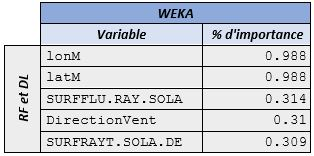
\includegraphics{img/ImpVweka.JPG}
    }
    \parbox{5cm}{
    \caption{ Variables importantes pour les algorithmes RF, et DL sous WEKA}
    \label{fig:wekaImp}
}
\end{figure}

 Le tableau illustré sur la figure \ref{fig:wekaImp} les variables importantes pour l’estimation de la visibilité horizontale avec les deux algorithmes \textit{Random Fores}t et \textit{Deep Learning} sous la plateforme \textit{WEKA}. Cette table montre que la pondération est la même pour les deux algorithmes.\\
 
 \ding{230} On constate que l'implémentation des algorithmes sous la plateforme \textit{WEKA} donne l'importance pour les mêmes variables lors du développement des algorithmes Datamining \textit{Random Forest} et \textit{Deep Learning}. Ainsi, la position géographique (latM et lonM) vient en tête des paramètres importants et ceci peut être justifié par le fait qu'on est en train d'étudier un problème de régression à caractère spatial. En fait, on cherche à estimer la visibilité sur un large domaine. Ensuite, on trouve deux paramètres importants et qui impactent largement l'occurrence de la visibilité réduite (vent et rayonnement).\\
 
Le tableau illustré sur la figure \ref{fig:impVar} dresse les cinq variables les plus importantes pour l’estimation de la visibilité horizontale avec les trois algorithmes ensembliste \textit{Random Forest}, \textit{Gradient Boosting Machine} et \textit{XGBoost} en utilisant les plateforme \textit{Scikit-learn} et \textit{H2O}. Il est à noter que pour le \textit{Deep Learning}, seule la plateforme \textit{H2O} offre la possibilité de mettre en évidence l'importance des variables en entrée.

\begin{figure}[!h]
    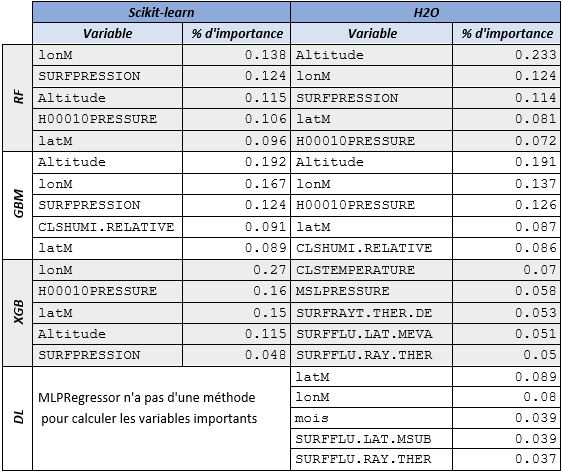
\includegraphics{img/ImpV.JPG}
    \caption{Variables importantes des algorithmes RF, GBM et XGB sous Scikit-learn et H2O}
    \label{fig:impVar}
\end{figure}

\ding{230} On constate que l'implémentation des algorithmes sous la plateforme \textit{H2O} et \textit{Scikit-learn} donne l'importance pour diverses variables lors du développement des algorithmes Datamining. Ainsi, on retrouve souvent la position géographique (latM, lonM, AltM et surface) et ceci peut être également justifié par le fait qu'on est en train d'étudier un problème de régression à caractère spatial. En fait, on cherche à estimer la visibilité sur un large domaine. Ensuite, on trouve des paramètres importants et qui impactent largement l'occurrence de la visibilité réduite à savoir les température et l'humidité à 2m ainsi que la pression au niveau de la surface et le rayonnement.\\






\newpage
\chapter*{Conclusion et perspectives}
\mtcaddchapter[Conclusion et perspectives]
\label{chap:conclusion}
La réduction de la visibilité horizontale est un facteur important d'accidents dans les divers secteurs de transport, en particulier l'aéronautique. Elle peut générer des dégâts financiers et humain considérables. D'où la prévision de la visibilité sera  d’un  grand  apport  pour  les  prévisionnistes météorologiques afin de minimiser et réduire les perturbations touchant les secteurs aérien, maritime et routier. Dans la littérature, diverses plateformes et algorithmes open-source ont été utilisés pour l’estimation de la visibilité selon diverses approches  (classification  et  régression). Ainsi, les performances des modèles développés différent d’une étude à une autre. L'objectif de ce stage est d'étudier la sensibilité de la performance des modèles développés à la plateforme et l'algorithme Datamining utilisés.\\


Afin d'atteindre notre objectif, certaines méthodes de Datamining sont appliquées aux sorties du modèle de prévision numérique du temps AROME, sous différentes plateformes open-source (\textit{Scikit-learn}, \textit{H2O}, \textit{WEKA}, \textit{Tensorflow} et \textit{Keras}) pour estimer la visibilité horizontale. Ainsi la base de données utilisée couvre 3 années de données horaires, répartie en 70\% pour l’apprentissage et 30\% pour le test afin d'évaluer la performance des algorithmes développés. Cet échantillonnage a été effectué de telle façon de garantir la représentativité des mois, des heures et des diverses classes de visibilités pour toutes les stations synoptiques utilisés dans les deux fichiers de données (test et apprentissage). Du côté outil de développement, nous avons opté pour une approche d'estimation par régression pour l'estimation de la visibilité horizontale. Ainsi, deux familles d'algorithmes du Datamining purement distinctes ont été employés: méthodes ensembliste incluant \textit{Random Forest}, \textit{Gradient Boosting Machine} et \textit{eXtreme Gradient Boosting} et l'apprentissage profond \textit{Deep Learning}.\\


Le développement et la modélisation des algorithmes Datamining a consisté dans un premier temps en l'utilisation de la configuration par défaut, puis dans l'étape suivante, nous avons réglé les hyper-paramètres en utilisant les deux techniques Grid Search et Random Search pour chaque algorithme Datamining utilisé dans cette étude sous divers plateformes open source. Ceci nous a permis d’obtenir le meilleur modèle pour un algorithme avec les hyperparamètres optimums.\\


L’analyse des résultats obtenus pour les déférents algorithmes utilisés sous les diverses plateformes, montre que la performance des modèles ensemblistes est la meilleure quelque soit la plateforme utilisée sauf pour \textit{Keras} où seul le \textit{Deep Learning} a été utilisé (plateforme considérée alors hors comparaison).  Ainsi, l’algorithme \textit{Random Forest} s’affiche comme meilleur estimateur de la visibilité après réglage des hyperparamètres pour les plateformes \textit{WEKA} et \textit{Scikit-learn}. Cependant, \textit{Gradient boosting machine} s’est distingué comme meilleur estimateur pour la plateforme \textit{H2O}. Les ordres de grandeurs des erreurs enregistrées sont similaires entre les diverses plateformes. Ainsi, on constate des erreurs quadratiques moyennes de 1933 m, 1942 m et 1945 m respectivement pour \textit{Gradient Boosting} sous \textit{H2O}, \textit{Random Forest} pour\textit{ Scikit-learn} et \textit{WEKA}. De même pour l’erreur absolue moyenne qui prend les valeurs suivantes 1199 m, 1221 m et 1232 m pour les mêmes algorithmes et plateformes.\\

Lors de la phase d'analyse croisée, nous  avons intégré  les hyperparamètres optimums obtenus soit par Grid search soit par Random search pour une plateforme donnée, dans le même algorithme mais pour une autre plateforme. Cette  approche  a  été  abordée  du  fait  que  lors  l’optimisation  des hyperparamètres, Grid Search permet de tester une série de paramètres et de comparer les performances pour en déduire le meilleur paramétrage. Or, Random Search est  une  technique  dans  laquelle  des  combinaisons  aléatoires  des hyperparamètres sont utilisées pour trouver la meilleure solution d’un modèle développé. Ainsi, il se peut que les hyperparamètres trouvés pour une plateforme donnée  ne  soient  pas  inclus  dans  la  fourchette  adoptée  pour  une  autre plateforme lors de la phase d’optimisation. On constate ainsi que les statistiques de la performance du modèle régresseur à base de \textit{Random Forest} et \textit{Gradient Boosting Machine} sont similaires. Pour \textit{eXtreme Gradient Boosting}, on constate que les statistiques de la performance du modèle régresseur se dégradent sous \textit{H2O}. Ainsi, on constate une dégradation de 222 m
en termes d’erreur quadratiques moyenne RMSE et un écart de 110 m en termes d’erreur absolue moyenne MAE. Pour le \textit{Deep Learning}, on a constaté que le changement de la plateforme impacte la performance du modèle régresseur pour les mêmes hyperparamètres.\\

L’analyse  comparative  par plateforme et par algorithmes  de l'importance des paramètres météorologiques a permis d'identifier ceux qui ont plus de poids lors l’estimation de la visibilité à partir des  prévisions  du  modèle  AROME. On constate ainsi que l’implémentation des algorithmes sous les plateformes utilisées donne l’importance pour diverses variables lors du développement des algorithmes Datamining. Ainsi, on retrouve souvent la position géographique
(latitude, longitude et Altitude) et ceci peut être justifié par le fait qu’on est en train d’étudier un problème de régression à caractère spatial. En fait, on cherche à estimer la visibilité sur un large domaine. Ensuite, on trouve des paramètres importants et qui impactent largement l’occurrence de la visibilité réduite à savoir les température et l’humidité à 2m ainsi que la pression au niveau de la surface et le rayonnement.\\

Les résultats de cette étude sont encourageants cependant il est utile de rappeler certaines limites de cette dernière et de citer certaines perspectives qui restent à explorer. Notre étude s’est focalisée sur une durée d'étude de 3 ans, ainsi il serait intéressant d’augmenter la durée de notre étude, aussi il sera d'un grand apport d'évaluer la sensibilité de la performance des modèles développés aux plateformes et algorithmes Datamining pour un cas de classification. D'autre part, il serait judicieux d'évaluer objectivement les plateformes à la base des indices appropriés. Enfin il serait judicieux d’évaluer l’apport d’autres plateformes open source.

\markboth{}{}
\newpart{Annexes}
\markboth{Annexes}{Annexes}
\appendix


\chapter{Code source des algorithmes développés sous Scikit-learn}
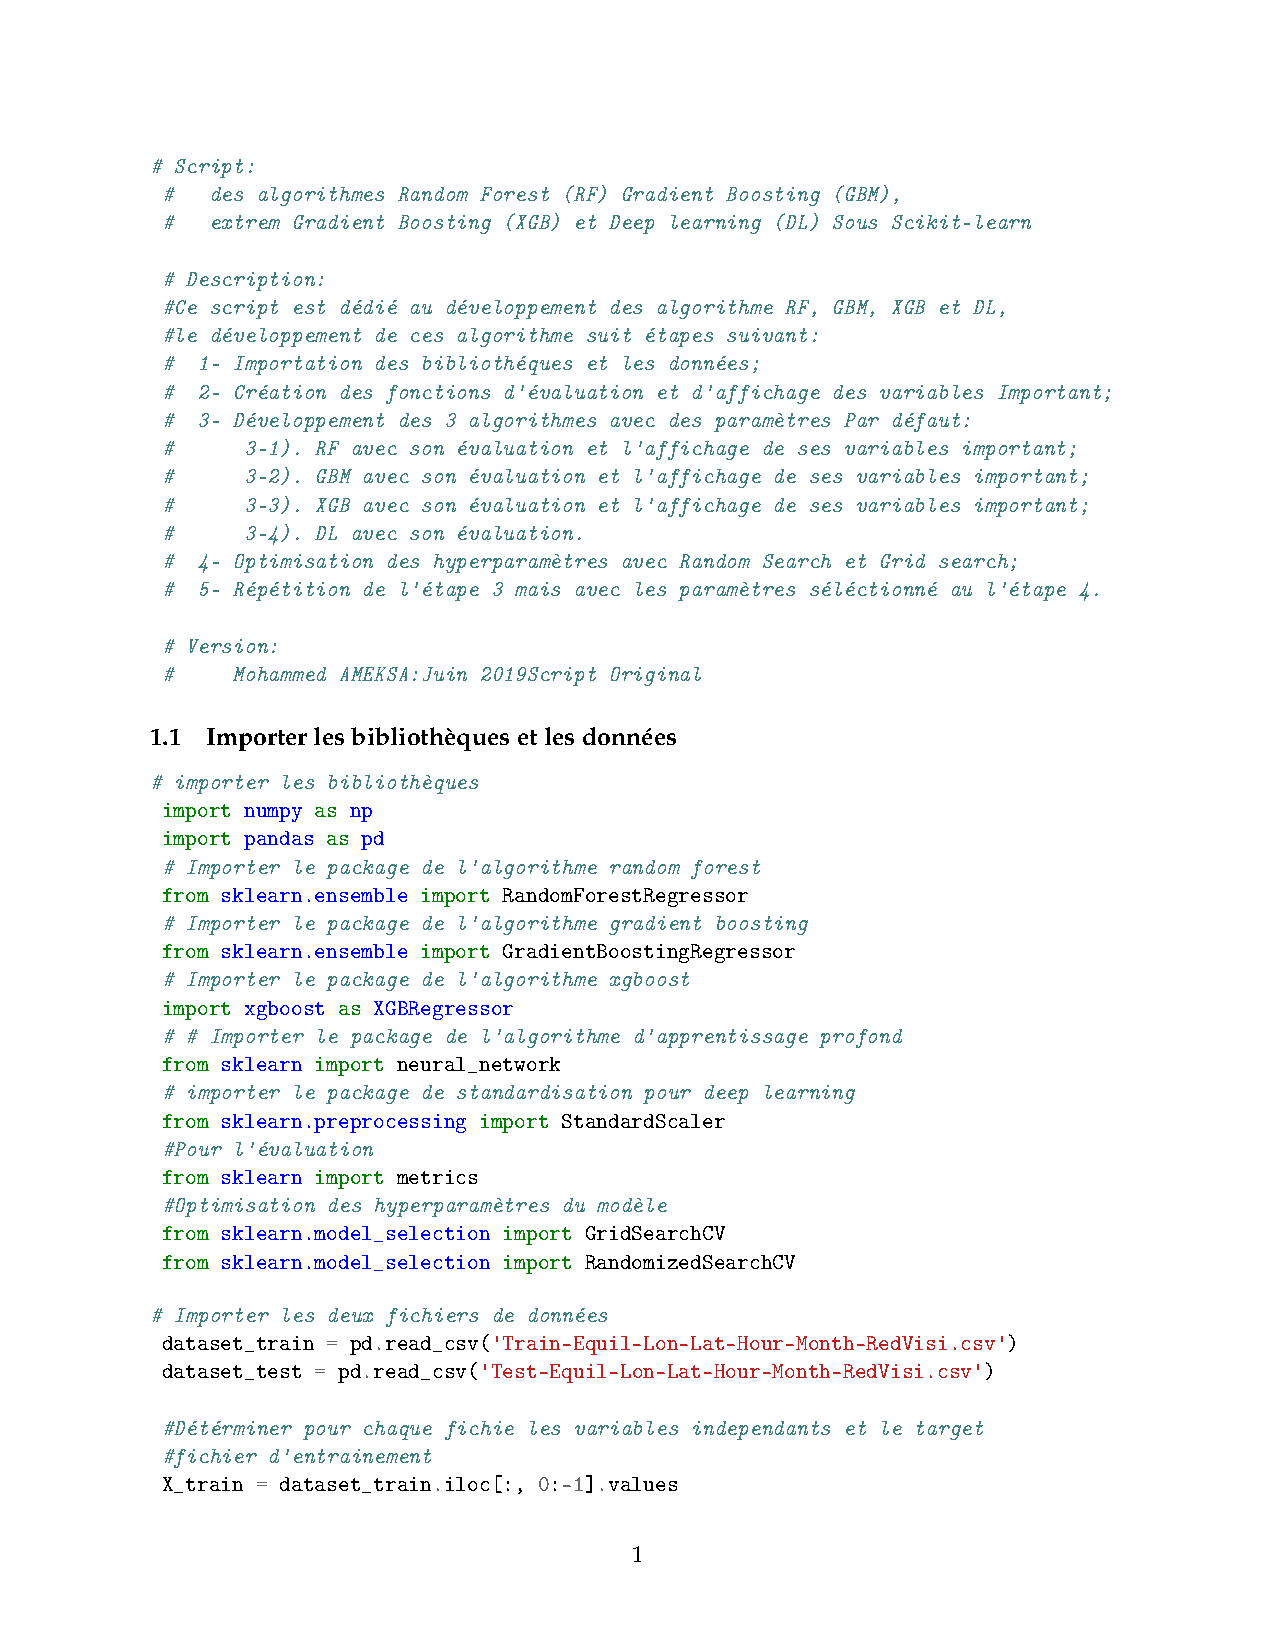
\includepdf[pages=-]{Annex/Scikit.pdf}

\chapter{Code source des algorithmes développés sous H2O}
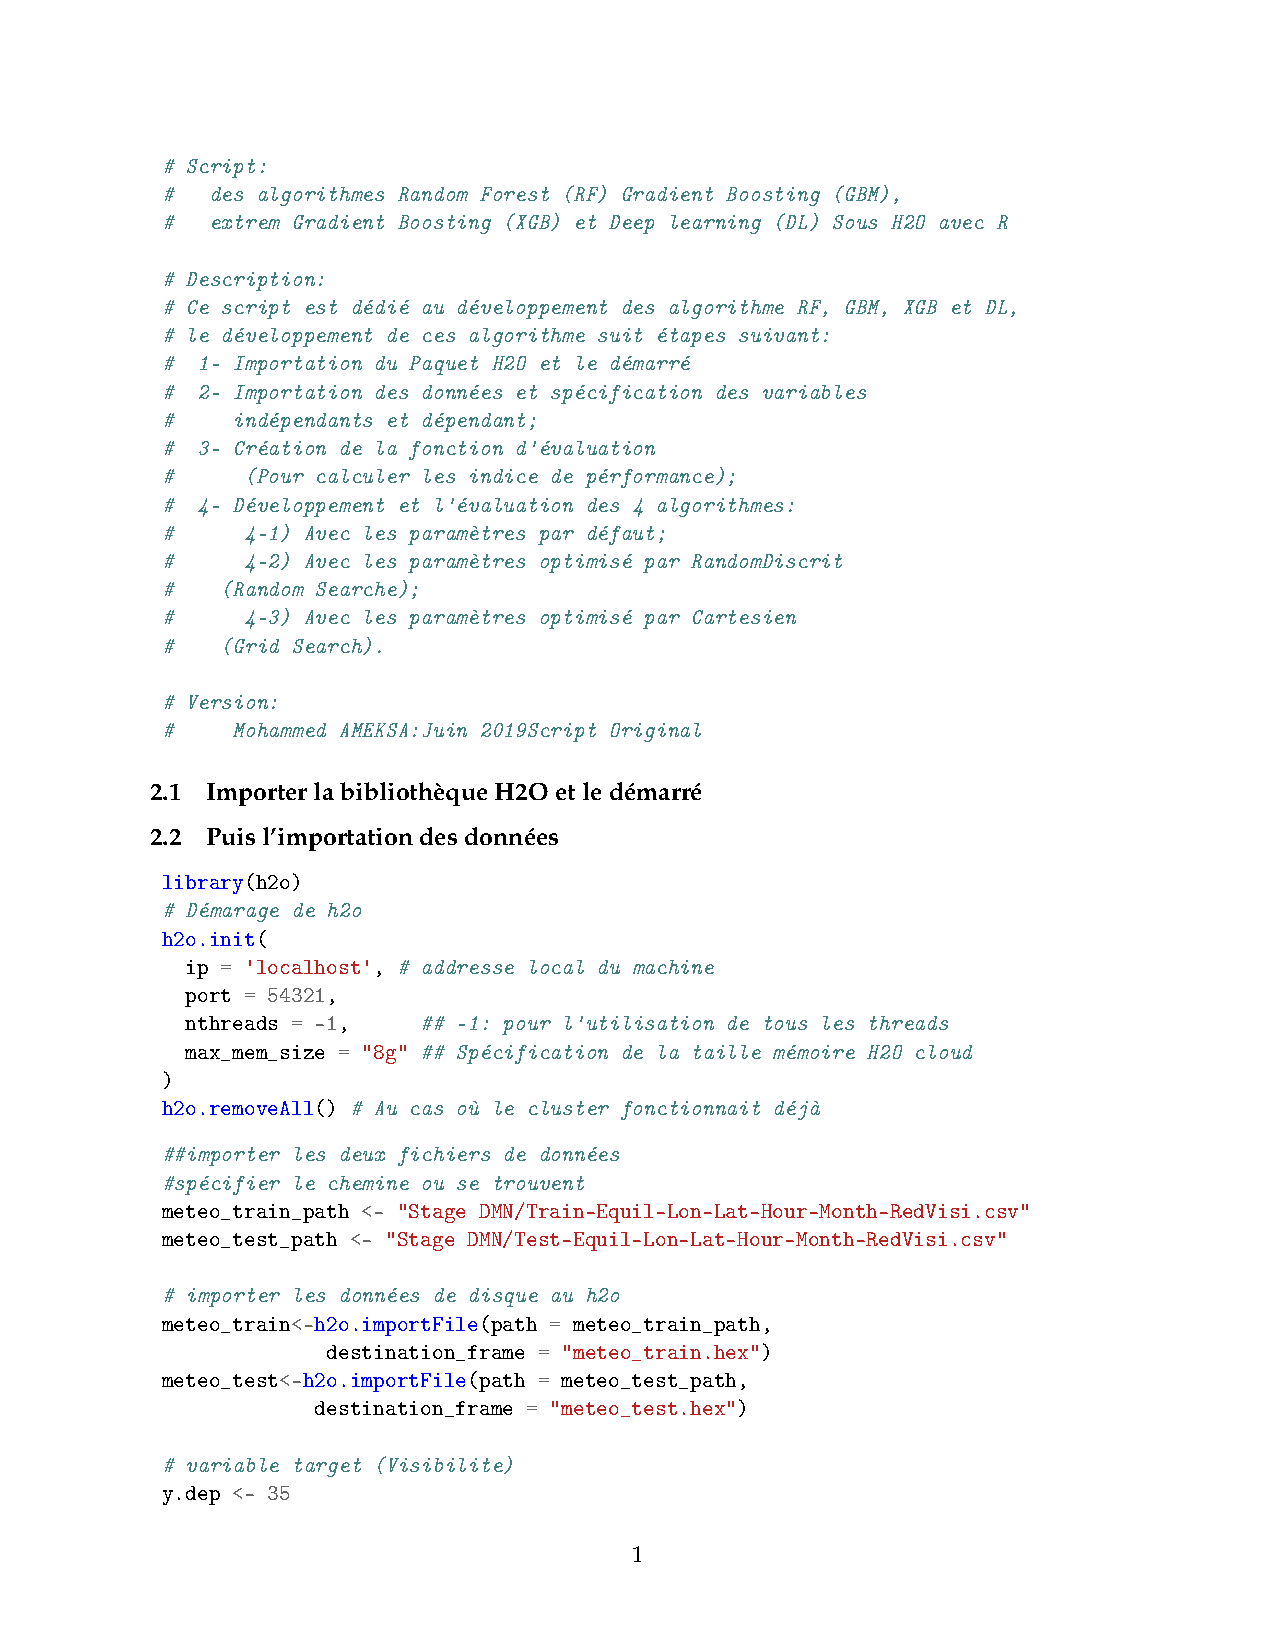
\includepdf[pages=-]{Annex/H2O.pdf}

\chapter{Code source de l'algorithme Deep Learning sous Keras}
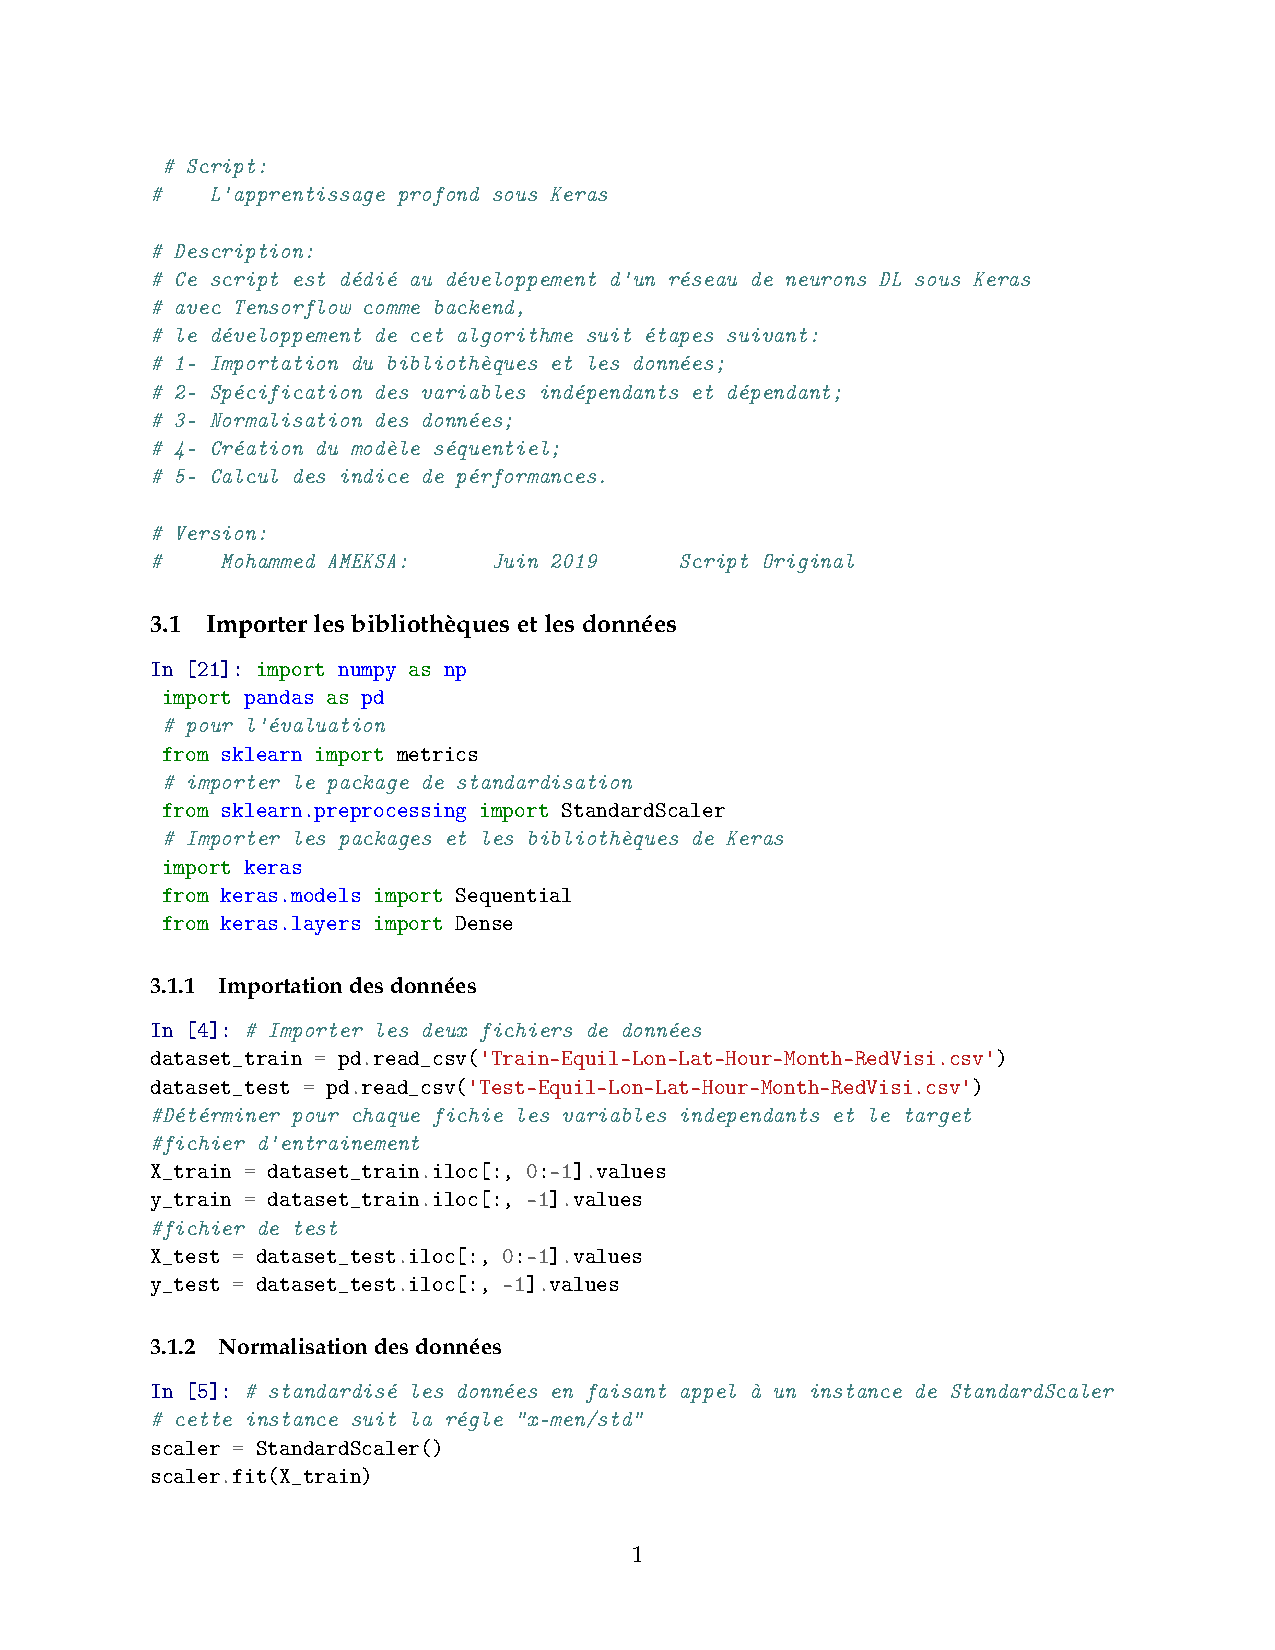
\includepdf[pages=-]{Annex/keras.pdf}

\chapter{L'éxécution de l'algorithme Random Forest sous WEKA}
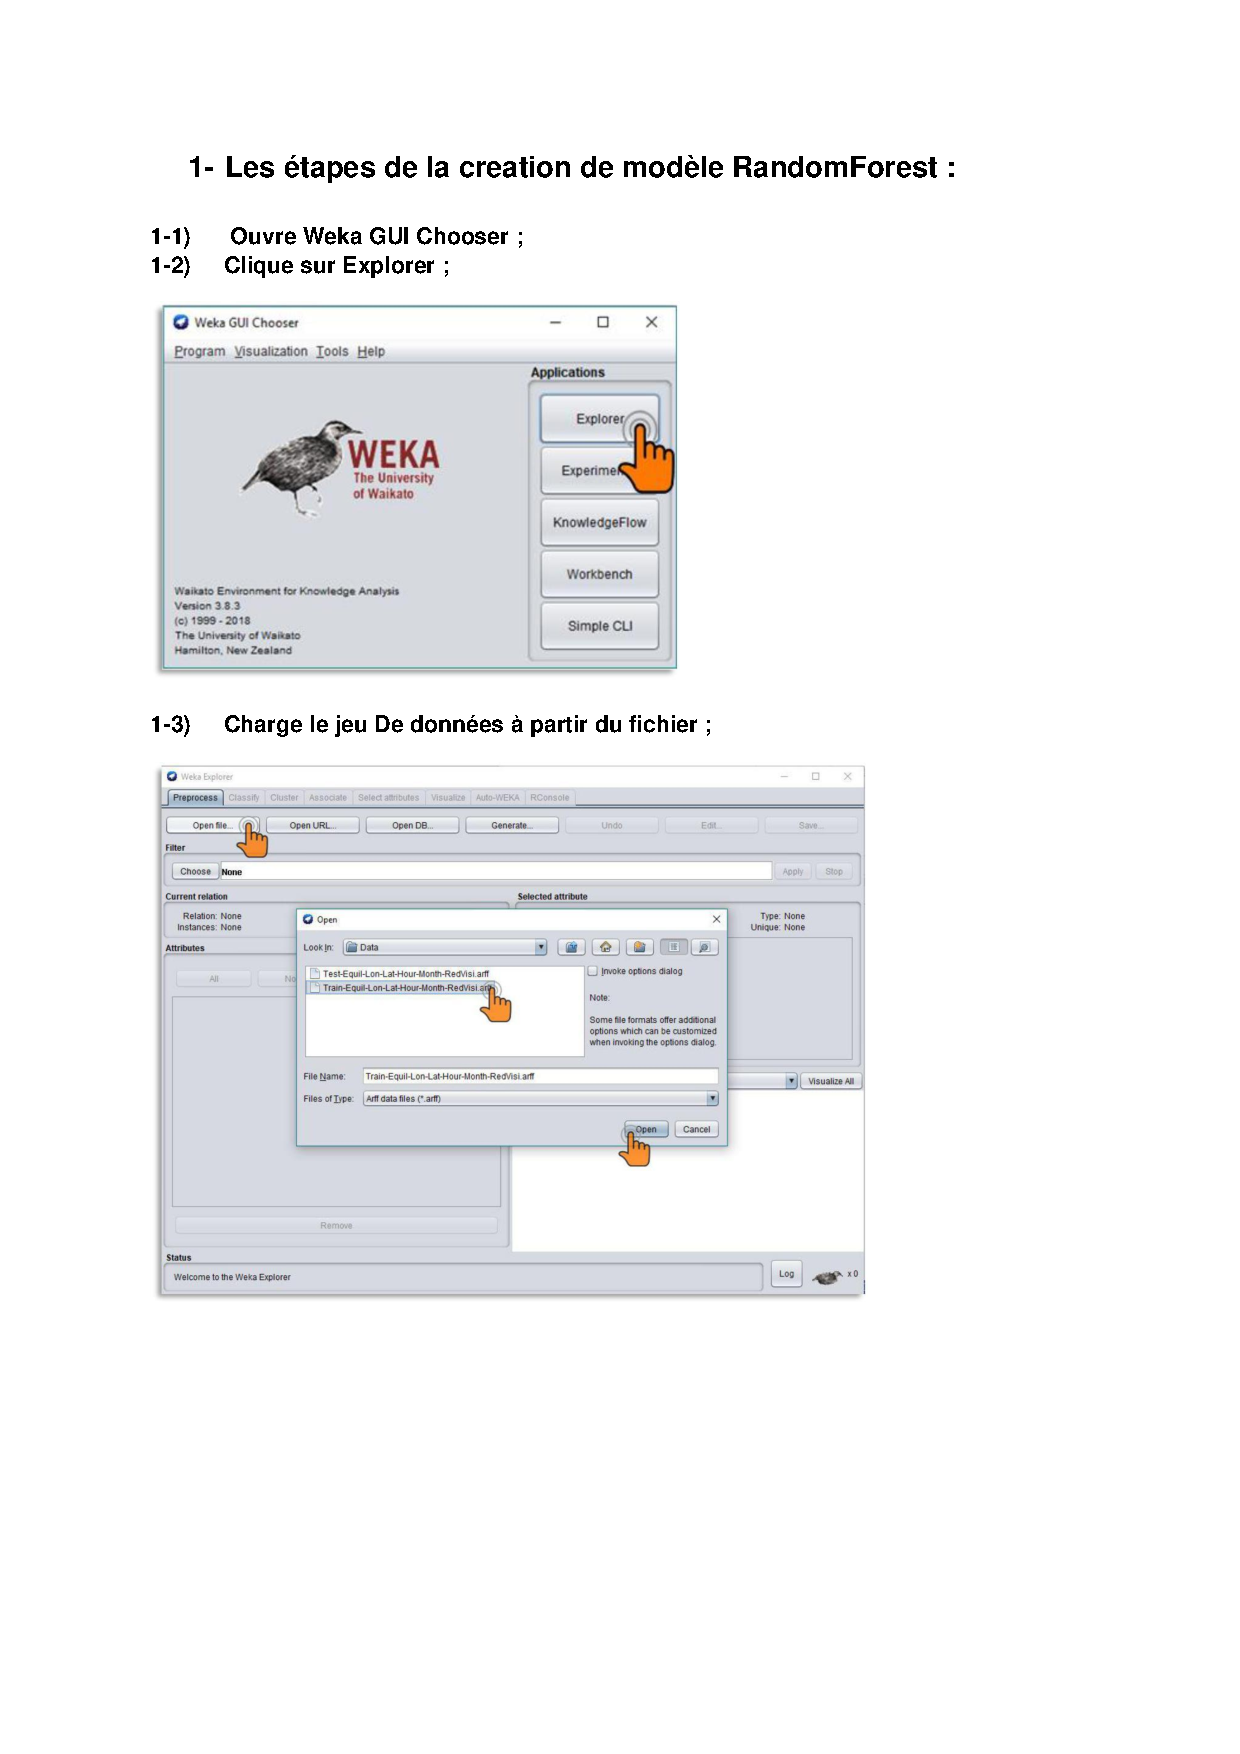
\includepdf[pages=-]{Annex/WEKA.pdf}


%BIBLIOGRAPHY
\backmatter
\cleardoublepage
%\thispagestyle{plain}
\adjustmtc

%\bibliographystyle{apalike}
\bibliographystyle{plainnat}
\bibliography{biblio.bib} 
\end{document}
